% Tento soubor nahraďte vlastním souborem s obsahem práce.
%=========================================================================
% Autoři: Michal Bidlo, Bohuslav Křena, Jaroslav Dytrych, Petr Veigend a Adam Herout 2019

% Pro kompilaci po částech (viz projekt.tex), nutno odkomentovat a upravit
%\documentclass[../projekt.tex]{subfiles}
%\begin{document}

% TODO: Kde rict ze implementovany zaznamnik je konkretne na seriovou komunikaci - vylozene UART? 

\chapter{Úvod}
\label{uvod}
Tato bakalářská práce je věnována návrhu a implementaci digitálního záznamníku s autonomním dokončením záznamu dat při výpadku napájecího napětí. Požadavek na zařízení vznikl od firmy NXP Semiconductors, konkrétně od týmu zaměřeného na bezdrátové nabíjení, ve kterém pracuji. Tento tým působí v České republice, jak v Rožnově pod Radhoštěm, tak i v Brně, a zároveň má své zastoupení v Asii a Severní Americe. NXP Semiconductors je jedním z předních členů WPC (Wireless Power Consortium), organizace zodpovědné za definování standardu Qi pro bezdrátové nabíjení. Primární zaměření NXP v této oblasti spočívá ve vývoji referenčních designů pro automotive sektor, kde zákazníkům poskytuje řešení určená pro integraci do vozidel.

Zákazníci, kteří využívají referenční designy NXP, pocházejí z celého světa a dostávají téměř hotový produkt, který lze následně certifikovat v Qi certifikačních laboratořích. Nicméně i přesto, že jsou referenční designy navrženy podle nejnovějších standardů, často dochází k jejich úpravám podle specifických požadavků zákazníků, zejména s ohledem na konkrétní poptávku koncového zákazníka (OEM – Original Equipment Manufacturer). Tyto požadavky jsou obvykle shrnuty v RFP (Request for Proposal), kde zákazník specifikuje konkrétní požadavky na systém. Tyto úpravy mohou být například realizovány z důvodu snížení ceny nebo zlepšení výkonu, například EMC charakteristik a nebo speciální chování bezdrátové nabíječky v krajních situacích. 

Při jakýchkoli úpravách však vznikají nové technické výzvy, a proto NXP poskytuje zákazníkům plnou technickou podporu až do úspěšné certifikace. Certifikace probíhá v různých laboratořích po celém světě, avšak ne vždy může být přítomen zaměstnanec NXP, který by dohlížel na celý proces a zajistil, že certifikace proběhne hladce. V těchto případech se momentálně tým pro bezdrátové napájení spoléhá pouze na záznamy poskytnuté operátorem certifikační laboratoře. Tyto záznamy však pocházejí pouze ze strany přijímače – tedy certifikačního zařízení, zpravidla od výrobců nok9 nebo Granite River Labs (GRL). Ty poskytují některé z důležitých informací, bohužel tyto nabídnuté záznamy nezahrnují explicitní informace o chování vysílače. Pokud tedy bezdrátová nabíječka, respektive bezdrátový vysílač, neprojde některým z testů, bývá často obtížné zpětně určit příčinu problému. Právě z tohoto důvodu vznikla potřeba záznamníku dat, který umožňuje zaznamenávat data přímo ze strany bezdrátové nabíječky a následně je porovnat s údaji získanými z testovacího zařízení. \cite{nxp_wireless_charging_team}

Návrh a implementace záznamníku musí reflektovat požadavky na snadnou obsluhu, neboť zařízení bude poskytováno zákazníkům pro již zmíněné účely certifikace. V klasickém scénáři zákazník předá nabíječku i se záznamníkem operátorovi certifikační laboratoře, ten si záznamník připojí k testovanému zařízení. Po skončení testovacího dne operátor záznamník vrátí zákazníkovi, který jej následně připojí k počítači a odešle společnosti NXP Semiconductors získané záznamy.

Z hlediska textové struktury se tato bakalářská práce, kapitola~\ref{zaznam_dat} se zabývá problematikou záznamu dat z historického i technického hlediska. Popisuje vývoj záznamových systémů od mechanických a analogových zařízení až po moderní digitální řešení. Dále se zaměřuje na principy digitálního záznamu, popisuje základní architekturu digitálních záznamníků a klíčové koncepty, které se uplatňují při jejich návrhu a implementaci.

Kapitola~\ref{navrh_digitalniho_zaznamniku}  je věnována procesu návrhu digitálního záznamníku. V úvodu kapitoly jsou rozebrána existující řešení z oblasti záznamu dat, která jsou podobná zařízení vyvíjenému v této bakalářské práci, a zároveň poskytují přehled o jejich výhodách a omezeních. Následně jsou představeny jednotlivé hardwarové a softwarové komponenty, které byly brány v úvahu pro implementaci digitálního záznamníku, přičemž u každé části systému je uvedeno vícero alternativ (byť nejde o jediná možná řešení). V závěru kapitoly je pak popsána výsledná architektura záznamníku, která prezentuje konkrétní komponenty vybrané ze širšího spektra možností.

% Tato deska doplňuje funkcionalitu základové vývojové platformy o prvky nezbytné pro spolehlivý provoz záznamníku, zejména o detekci výpadku napájecího napětí, zálohované napájení pomocí superkondenzátorů a generování stavových signálů pro uživatele. Součástí expanzní desky jsou také externí komponenty, jako je reálný časový obvod (RTC), nezbytný pro přesné časové značky v uložených datech. Celkově tato deska výrazně rozšiřuje schopnosti základní desky a tvoří nezbytný předpoklad pro správnou funkčnost celého systému.
Kapitola~\ref{realizace_hardwaru} se zaměřuje na realizaci hardwarové části digitálního záznamníku v podobě dedikovaného zařízení. Klíčovým prvkem této části je návrh a realizace rozšiřující expanzní desky, která byla navržena speciálně pro potřeby tohoto projektu.

% ... navržena speciálně pro potřeby tohoto projektu. Závěrečná část kapitoly je věnována mechanickému návrhu zařízení, konkrétně popisu návrhu ochranného krytu.
% chranici proti kontaktu s zivymi castmi zaznamniku

Kapitola~\ref{softwarova_implementace} je věnována implementaci firmwaru digitálního záznamníku. Kapitola popisuje návrh a realizaci jednotlivých částí firmwaru, který zajišťuje funkci zařízení jako autonomního záznamového systému. První část kapitoly se zaměřuje na samotný mechanismus záznamu dat, tedy příjem, zpracování a ukládání zaznamenaných dat. Následuje popis implementace mechanismu pro zpřístupnění uložených dat uživateli bez nutnosti fyzického vyjmutí paměťového média. V závěrečné části je popsána logika detekce ztráty napájecího napětí a logika signalizace stavu zařízení vůči uživateli.

Kapitola~\ref{testovani_systemu} popisuje proces, jakým bylo zařízení testováno a validováno. Primárně se zaměřuje na funkcionální testování zařízení, tj. ověření, že systém vykazuje správné chování. Další část je věnována kontrole bezpečnosti a spolehlivosti implementovaného kódu.

V závěru v kapitole~\ref{zaver} jsou zmíněna možná rozšíření digitálního záznamníku a zhodnocení práce.

\chapter{Záznam dat}
\label{zaznam_dat}

\section{Historické pozadí záznamu dat}
\label{pocatky}
Lidstvo již od svých počátků mělo potřebu zaznamenávat data, neboť člověk mnohdy dokáže datům přiřadit sémantiku -- jejich význam, a proměnit je tak v informace. Právě díky nim se lidé mohou učit z minulých zkušeností, předávat znalosti dalším generacím, organizovat a podpořit tak neustálý lidský pokrok. 

% Nicméně největším pokrokem ve zaznamenávání dat nastal s příchodem výpočetní techniky.
Po staletí byl záznam dat výhradně manuální. Informace se uchovávaly v rukopisech, knihách či na papírových svitcích, ať už formou psaného textu, nebo ručně zapisovanými výsledky pozorování. Zaznamenaná data byla však limitována svou přesností, která byla omezena lidskou obsluhou a možnostmi mechanick  ých nástrojů, tak i svou dostupností, protože k nim měl přístup jen omezený okruh lidí.

% Přesnost zaznamenaných dat byla však omezena schopnostmi lidské obsluhy a možnostmi mechanických nástrojů, tak i omezenou dostupností, 
% ale také dostupnost těchto dat byla omezena, ke kterým měl přístup jen omezený okruh lidí.


% pripadne to upravit na: Stěžejní změna přišla ve 20. století s rozvojem automatických záznamníků
Stěžejní změna přišla na konci 19. století s rozvojem elektrotechniky a nástupem automatických záznamníků, které umožnily jednoduchý sběr dat bez nutnosti lidského zásahu. Namísto ručně zapisovaných měření začaly být hodnoty přenášeny přímo do záznamových zařízení, která je dokázala systematicky uchovávat. \cite{origin_of_chart_recorders}

\begin{figure}[h] % obrazek patent
    \centering
    \includegraphics[width=0.40\textwidth]{obrazky-figures/first_chart_recorder.png}
    \caption{První skutečný grafický záznamník (Chart Recorder) patentovaný Williamem Henrym Bristolem v roce 1888 \cite{bristol_chart_recorders}}
    \label{fig:chart_recorder}  
\end{figure}

\section{Záznam dat v počátcích elektrotechniky}
\label{zaznam}
Prvními specializovanými záznamníky byly mechanické či elektromechanické zařízení, využívající principu analogového záznamu dat. Jejichž primárním účelem bylo zaznamenávání fyzikálních veličin, jako je například teplota, tlak, vlhkost nebo vibrace. Tyto přístroje využívaly myšlenky mechanického pohyblivého pera, které převádělo naměřenou hodnotu fyzikální veličiny na samočinný pohyb. Pro realizaci tohoto pohybu bylo nutné nejprve převést měřenou fyzikální veličinu na mechanický posun, přičemž konkrétní způsob převodu závisel na typu měřené veličiny. Například pro měření teploty se běžně využíval bimetalový pásek, složený ze dvou kovových materiálů s různou hodnotou teplotní roztažitelnosti. Při změně teploty docházelo k prohnutí pásku v důsledku rozpínání kovu, čímž bylo rozpohybováno mechanické pero, které zapisovalo hodnotu na paměťové médium. 

% mechanicky -< samocinny
% pomocí kterého se zapisovala změřená hodnota na paměťové médiu (papírová páska nebo papírový buben)

\begin{figure}[h] % obrazek polygraf
    \centering
    \includegraphics[width=0.50\textwidth]{obrazky-figures/polygraaf.png}
    \caption{Ukázka zařízení patřící do skupiny analogových záznamníků - polygraf \cite{polygraph_picture}}
    \label{fig:polygraaf}
\end{figure}


Tyto přístroje jsou běžně používány od druhé poloviny 19. století. Pro již zmíněný záznam teploty je možné například využít přístroj zvaný cirkulární grafový záznamník (Circular Chart Recorder), dále je hojně využíván polygraf, využívaný jako detektor lži. Značnou nevýhodou těchto záznamníků bývá typ paměťového média, na které probíhá zápis hodnot, nejčastěji jim je papírová páska nebo papírový buben. Nevýhodou těchto paměťových médií je nutnost jejich časté výměny za nové, ještě nepopsané, jelikož výsledné záznamy by se jinak staly značně nepřehlednými, pokud by byly popsány vícekrát. \cite{origin_of_chart_recorders}

Hlavním omezením analogových záznamových systémů je jejich vysoká specializace\footnote{Řešení jsou současně mnohdy optimalizovaná pro záznam konkrétního systému.} pro jediný konkrétní typ záznamu. Tyto záznamníky nejsou snadno upravitelné pro jiné účely, na rozdíl od digitálních řešení, která umožňují flexibilnější přizpůsobení (například pouhou úpravou softwarového programu) k sledování monitorované soustavy. Často je v těchto případech nutné využít jiné analogové řešení. \cite{analog_signal_and_digital_signal_processing_Tel_System}

Další limitací těchto přístrojů je ruční vyhodnocování dat, což je mnohdy časově zdlouhavé a také náchylné k chybám. K správné interpretaci dat je pak často potřeba zkušená obsluha a v některých případech i pomocné měřící pomůcky. Přenos dat a automatizace taktéž byly komplikované, proto jakmile se v polovině 20. století začaly na trh dostávat číslicové systémy, analogové záznamové systémy těmito digitálními systémy byly postupně nahrazovány. \cite{newcastle_history_of_digital_computers, florian_prechod_a_analog_do_digital, rcp_analog_vs_digital}

%Jak obecne probiha princip digitalniho zaznamu dat, co jsou to digitalni data, ze se v dnesni dobe uprednostnuje tento zpusob misto analogoveho zaznamu.

% TODO: Kde napsat co je to vubec zaznamnik? Ze je to pristroj, ktery zpracovava, uklada a pripadne analyzuje data...
\section{Digitální zpracování dat}
\label{digitalni_zaznam_dat}
S nástupem číslicových systémů v polovině 20. století došlo k velkému pokroku ve způsobu, jakým byla data zaznamenávána, zpracovávána a uchovávána. Digitální zpracování dat v porovnání s analogovým zpracováním se liší způsobem, jakým se v systému obecně pracuje se signály (viz. \ref{zaznam}). Zatímco analogový záznam pracuje se spojitými (kontinuálními) signály, digitální záznam využívá diskrétní (číslicové) hodnoty, které jsou uchovávány v binární podobě.

\subsection{Princip d   igitálního záznamu dat}
Z předchozího textu je tedy zřejmé, že digitální zpracování dat (tedy i záznam dat) vyžaduje číslicové hodnoty a z toho plyne, že již na vstupu musí být příchozí signály v digitální podobě. Data tedy musí být generována číslicovými zdroji, nebo musí být převedena do digitálního tvaru pomocí komponenty k tomu určené, kterou je například analogově-digitální převodník.

Pro převod analogových signálů do jejich digitální podoby se využívá proces digitalizace, který zahrnuje tři základní kroky. V počátku dochází ke vzorkování, při kterém je původní spojitý signál snímán ať už v pravidelných či nepravidelných časových intervalech. Následně dochází ke kvantizaci, při níž jsou vzorkované hodnoty zaokrouhleny na nejbližší úroveň amplitudy v omezeném rozsahu. Vzorky jsou tedy rozděleny do segmentů (tříd) diskrétních hodnot, přičemž tento krok s sebou nese ztrátu přesnosti závislou na jemnosti stupnice, která se nazývá kvantizační chyba. Nakonec je kvantizovaný signál kódován do binární podoby, ve které jej může výpočetní stroj dále zpracovávat, ukládat nebo přenášet.

\begin{figure}[h]
    \centering
    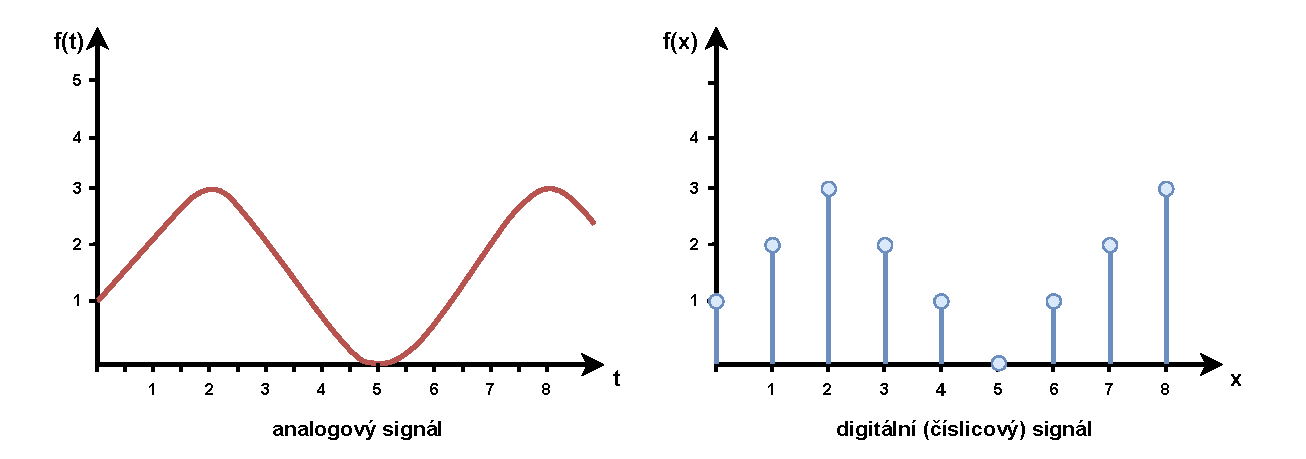
\includegraphics[width=1.00\textwidth]{obrazky-figures/digital_vs_analog.pdf}
    \caption{Průběh analogového a digitálního signálu}
    \label{fig:digital-vs-analog}
\end{figure}

U digitálních signálů je proces záznamu výrazně jednodušší, protože již nevyžaduje žádnou digitalizaci. Digitální data vstupující do záznamníku v podobě datového toku (data stream) skrz přijímací periferie. Tyto periferie nejsou navrženy pro přímé měření konkrétních fyzikálních veličin, ale pro příjem napěťového signálu reprezentujícího data dle přesně definovaného formátu. Typicky se jedná o digitální rámce, v nichž jsou data zakódována podle určitého přenosového schématu, například rámec může obsahovat jeden start bit, osm datových bitů a jeden stop bit, jako je to v případě UART přenosu. Tedy jedna periferie může přenášet jak údaje o teplotě, vlhkosti, tak i cokoliv jiného, pokud je dodržen rámec, přičemž povaha přenášených dat závisí na senzorech či zařízeních připojených k této periferii. Přijímaná data jsou tedy v přijímací periferii zpracovávána přímo ve své binární podobě a mohou být bez nutnosti další konverze zpracovávána, přenášena či ukládána.

Digitální záznam poskytuje mnoho výhod oproti svému analogovému protějšku. Primárně je to jeho flexibilita a efektivita při zpracování, ukládání a přenosu dat. Digitální data lze snadněji kopírovat, přenášet, zpracovávat a ukládat, což je pro záznamové systémy zásadní. Díky digitálnímu záznamu můžeme dnes i jednoduše analyzovat data v porovnání s analogovým záznamem.  Významnou výhodou digitálního záznamu je také vyšší přesnost, neboť odstraňuje chyby způsobené lidskou interpretací a umožňuje zachycení i těch nejmenších odchylek. \cite{rcp_analog_vs_digital}
% ...  interpretací a umožňuje zachycení i těch nejmenších odchylek. Proto jsou dnes systémy s digitálním záznamem preferovanou volbou.

Pro svůj provoz však vyžadují spolehlivý zdroj elektrické energie, případně i stabilní připojení k síti, což může výrazně omezit jejich využití v odlehlých nebo energeticky nestabilních lokalitách. Zároveň jsou citlivé na výpadky napájení, selhání hardwaru či softwaru a v neposlední řadě i na kybernetické hrozby, při kterých může dojít ke ztrátě či poškození všech uložených. \cite{rcp_analog_vs_digital}
% pripadne k jejich uniku?

% TODO: Digitální záznamník může sloužit i pouze pro čistě PC programy? Pokud je zde nejak prijimaci periferie? To by slo primo do CPU
\subsection{Digitální záznamník}
\label{digitalni_zaznamik}
Digitální záznamník je dedikované zařízení nebo softwarový program určený ke sběru, zpracování a ukládání dat ve formě digitálního záznamu. Na základě analýzy běžně používaných digitálních záznamníků lze jejich architekturu zpravidla členit do tří základních komponent, kterými jsou přijímající periferie, procesorové jádro a úložiště (viz. obrázek \ref{fig:common-digital-datalogger}). \cite{researchgate_general_dataloggger_multiple_sdcards, ieee_digital_sound_recorder_arm_sd_card, ieee_multi_connectivity_datalogger_sd_card}

Prvním klíčovým prvkem digitálního záznamníku je vstupní periferie či rozhraní, které slouží ke sběru vstupních dat. Vstupní periferie, která může mít podobu fyzických periferií, například sériových komunikačních rozhraní (UART, SPI, I\textsuperscript{2}C a další), síťových rozhraní (Ethernet, Wi-Fi, LoRa a další) případně analogově-digitální převodníky. Může se jednat, ale také například o softwarová rozhraní, jako jsou například různá API (Application Programming Interface). \cite{fourcore_win_process_birth, ieee_digital_sound_recorder_arm_sd_card}

Druhým hlavním prvkem digitálního záznamníku je procesorové jádro či jádra centrální výpočetní jednotky (CPU), zajišťující zpracování vstupních dat. Procesorové jádro popřípadě jádra mohou být jak součástí mikrokontroléru, mikroprocesoru, tak i stolního počítače, které může mít v tomto případě na starosti jednoduché operace, jako je například přepočet hodnoty z analogově-digitálního převodníku na teplotu podle kalibrační křivky senzoru, přes filtrování šumu a doplňování časových značek k naměřeným vzorkům, až po pokročilé analýzy dat - například zpracování signálů pro EKG měření. \cite{springer_development_ECG_recorder}

\begin{figure}[h]
    \centering
    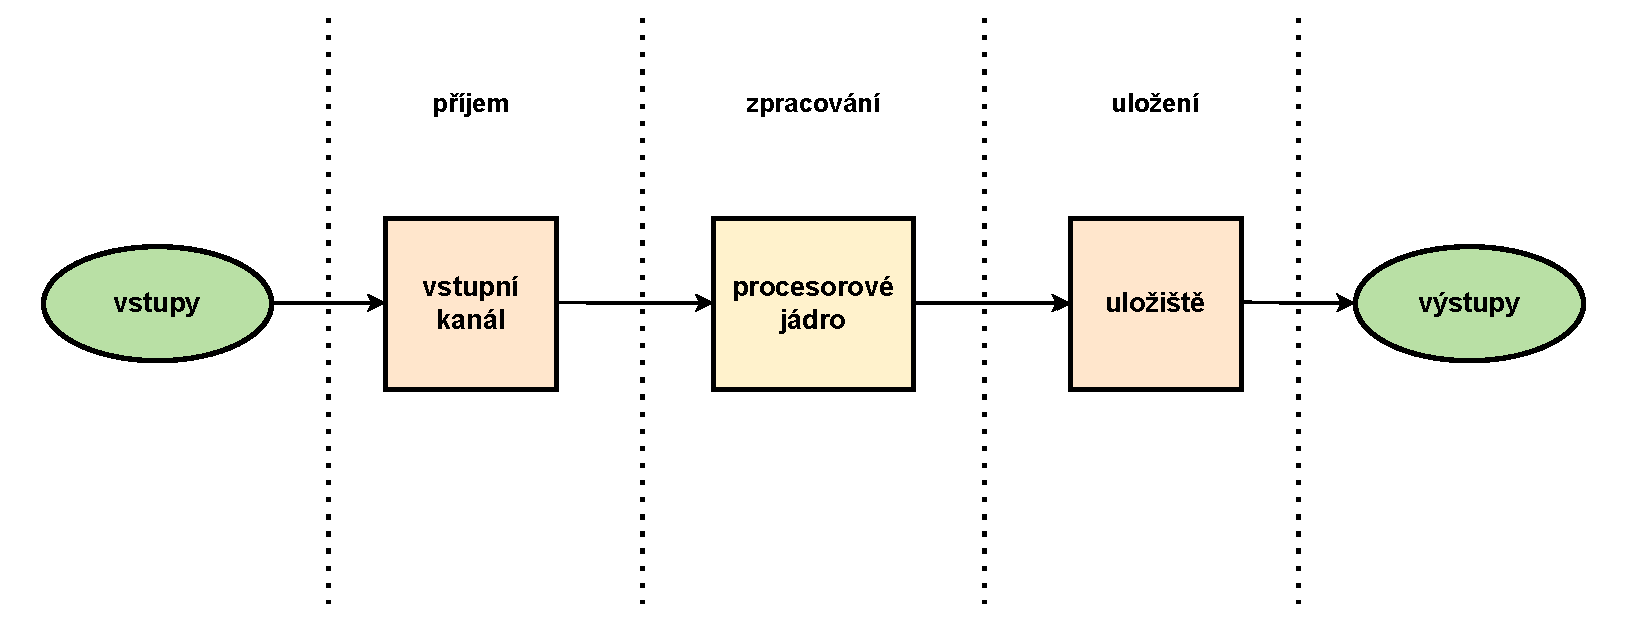
\includegraphics[width=1.00\textwidth]{obrazky-figures/common_digital_datalogger_scheme.pdf}
    \caption{Obecné schéma digitálního záznamníku}
    \label{fig:common-digital-datalogger}
\end{figure}

Poslední a také jednou z nejdůležitějších všeobecnou částí digitálního záznamníku je úložiště, kde jsou data ukládána pro pozdější přenos a zpracování (post-processing). Volba tohoto úložného prostoru závisí na požadavcích aplikace a rozsahu jejího využití, od osobních "hobby" projektů až po zařízení využívaná ve velkopodnikových prostředích, nasazována ve vysokých počtech. V závislosti na tom lze využít různé strategie, které jsou v koherenci s různými technologiemi od paměťových karet SD a eMMC přes interní RAM či flash paměti až po síťová úložiště a cloudové služby. V mnoha případech je také využíván hybridní přístup. Nashromžděná data mohou být nejprve ukládána do interní volatilní paměti záznamníku, jakou je třeba RAM úložiště (random access memory) a následně dávkově přenášena na trvalé médium (viz. kapitola \ref{fig:batch-processing}) v podobě lokálního či vzdáleného úložiště. Lze také přidat různé mezivrstvy pamětí, například feroelektrickou paměť s náhodným přístupem (FRAM), která je podrobněji rozebrána v kapitole \ref{fig:feram-1t-1c}, nebo jiné varianty nevolatilních pamětí s náhodným přístupem, případně další typy pamětí. \cite{rta_local_vs_cloud} 
% lokalni uloziste lze vyuzit i v kombinaci se vzdalznym ulozistem, kdy vznika hybridni architektura... 
% Zmiňované lokální uložiště lze navíc využít v kombinaci ze vzdáleným uložištem, kdy vzníká hybridní architektura, lze například data nejprve ukládat do interní paměti záznamníku (například RAM úložiště) a následně dávkově přenášena na trvalé médium (viz. kapitola \ref{fig:batch-processing}) nebo odesílána přes síť. \cite{rta_local_vs_cloud}

Digitální záznamník poskytuje výstupy, obvykle jimi jsou organizovaná data, která mohou být dále analyzována, vizualizována nebo zpracovávána jinými systémy. Jakou podobu mají výstupní data, tedy jaký je jejich formát, opět závisí na konkrétních požadavcích aplikace. Jedním z požadavků je volba dle typu úložiště, jedná-li se o lokální úložný prostor, například paměťovou kartu, využívají se velmi často typy formátů, jako třeba formát prostého textu (plain text) nebo binární formy. Databázová řešení typicky využívají formáty vycházející z relační nebo objektové reprezentace dat. Cloudová řešení naopak nabízejí daleko širší výběr, lze využít jak zmíněný prostý text, i binární formy, také lze ale využít objektové, textové formáty nebo formáty známé z databázových systémů. Dále záleží, jakým způsobem bude proveden přenos dat, pokud bude využita síťová komunikace, třeba pomocí MQTT či HTTP, je vhodné data uspořádat do serializované podoby, zatímco při zvolení přenosu po sériové lince je naopak vhodnější a efektivnější využít opět některý z binárních formátů. Důležitou roli hrají i požadavky na následný post-processing a interpretaci dat v jiných systémech či aplikacích k tomu určeným. Například pro náhled na digitální data z pohledu časových řad může být vhodné využít formáty, které jsou kompatibilní s například databázovými systémy k tomu určenými, jako je TimescaleDB, InfluxDB. V dalších případech může být efektivní využít knihovny pro zpracování a analýzu dat, například Pandas v prostředí Pythonu, které umožňují rychlou manipulaci s velkým objemem strukturovaných dat, v takových případech je tedy zase lepší strukturovat data podle formátu CSV. \cite{medium_optimalization_iot_data_storage_timescaledb}

Způsobů, jak lze digitální záznamník sestavit, existuje mnoho, přičemž volba konkrétní architektury závisí na požadavcích dané aplikace. Velice často se však skládá z výše představených komponent.

\subsection{Digitální záznam v počítačovém systému}
Digitální záznamníky lze implementovat na počítačových systémech, jako jsou osobní počítače či servery, v podobě softwarových řešení, sloužících ke sběru, zpracování a potenciální archivaci dat. Tyto systémy obvykle také vycházejí ze struktury obecného číslicového záznamníku, popsaného v kapitole \ref{digitalni_zaznamik}. 

% pseudo zarizeni - syslog
%  Syslogd to nasledne odesila do /var/log/
Vstupní data mohou například pocházet z periferií, jako je například síťová karta či sériové porty, ale mohou také pocházet ze vlastních komponent výpočetního stroje, "pseudo" zařízení obsahujících stavy aplikací běžících na daném počítači, "pseudo" soubory obsahující systémové informace.\footnote{Zmíněnené "pseudo" zařízení využívá například Syslogd, který shromažďuje zprávy, které systémové procesy a aplikace odesílají do pseudozařízení /dev/log. Naopak mezi "pseudo" soubory můžeme zařadit /proc, obsahující systémové informace za běhu, jakými jsou například systémá paměť, připojená zařízení, konfigurace hardwaru,...} A tato data lze obecně získat pomocí speciálních API (např. již zmiňovaných kernel API) či knihoven. Procesor, který tato data příjímá, tak je obvykle nejen zpracovává, ale často i určitým způsobem vyhodnocuje, jelikož disponuje dostatečným výpočetním výkonem pro pokročilé operace. Výsledkem těchto úkonů procesoru nad daty bývají informace o aktuálním stavu sledovaného systému, které lze využít k monitorování a dalším rozhodovacím procesům. \cite{linux_in_action_log_and_monitoring}

% Wireshark: RAM -> Export
% Terminal or Serial Dataloggers (COM, RS232,...) -> Export to File, Excel or Database
% 
Podle požadavků aplikace a jejího zaměření se liší i způsob, jakým jsou data uchovávána. Mnohdy si tyto záznamníky odkládají data pouze dočasně do operační paměti RAM, to umožňuje sledovat pouze aktuální stav nebo krátkodobé trendy. Pro sledování dlouhodobých trendů je pak možné tyto záznamy exportovat na dlouhodobá uložiště, do různých typů souborů - CSV, XLS či speciálních formátů relevantních dané aplikaci. Také lze uplatnit koncept exportování do databázových systémů a cloudových služeb.

Takovýmto záznamníkem či rovnou monitorovacím systémem může být například program Wireshark, sloužící k záznamu síťové komunikace na síťových rozhraních počítačového systému. Wireshark pro záznam síťových rámců neboli paketů využívá vícevrstvou architekturu, data přicházejí přes síťovou kartu, na hardwarové vrstvě. Pakety jsou následně zachytávány nebo dokonce i filtrovány pomocí WinPcap knihovny (\textit{Windows Packet Capture}). Následně jdou přijatá data paketů zpracovávaná, identifikována (přiřazena konkrétnímu protokolu) a vizualizována na aplikační vrstvě. \cite{researchgate_wireshark_architecture, wireshark_architecture_diagram}

\begin{figure}[h]
    \centering
    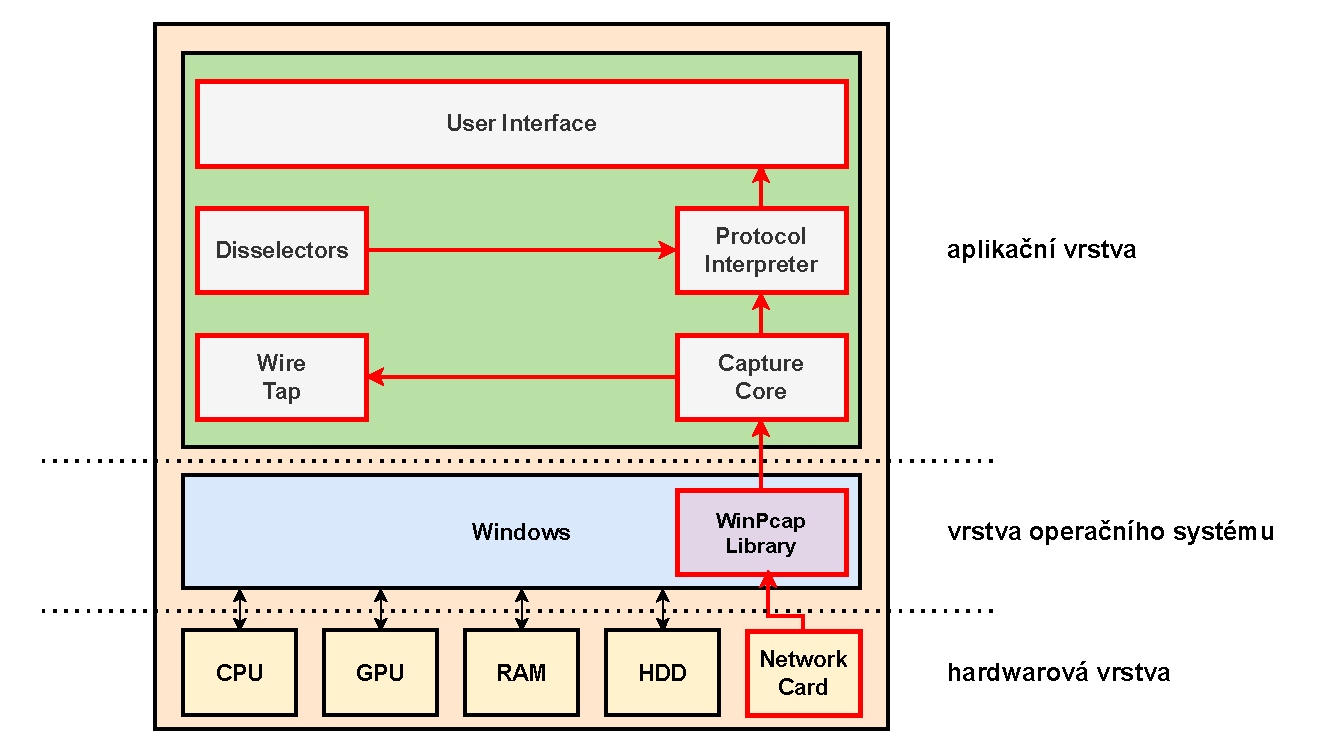
\includegraphics[width=1.00\textwidth]{obrazky-figures/wireshark.pdf}
    
    \caption{Schéma pokročilého digitálního záznamníku síťové komunikace - Wireshark \cite{researchgate_wireshark_architecture, winpcap_architecture}}
    \label{fig:computer-recorder}
\end{figure}

% Energie a udrzba?
Je nutné si uvědomit, že tyto záznamníky jsou především implementovány na strojích s relativně výkonnými hardwarovými prostředky, což je činí kolikrát až překvalifikované pro pouhé monitorování, proto se představují spíš jako doplněk, zatímco hlavním účelem stroje mohou být jiné (například vývoj síťové aplikace), přičemž tyto záznamníky mohou sloužit například k monitorování zmíněného síťového provozu, monitorování procesů běžících na daném stroji, pokročilé sériové záznamníky a terminály, či záznamníky speciálních rozhraní, jako je například HID (Human Interface Device).\footnote{Tyto záznamníky tedy nemusí sloužit pouze k monitorování samotného stroje na kterém jsou spuštěny, ale mohou také sledovat další připojená zařízení (a periferie), jakám je například sledování komunikace s mikrokontrolérem prostřednictvím sériového terminálu.}

Před implementací či použitím takového záznamníku je tedy vhodné si promyslet účel záznamníku. Klíčovou otázkou je, zda bude pro záznam nezbytné využít výpočetně výkonné zařízení (jakým je například stolní počítač), a zda zařízení bude sloužit výhradně k pořizování záznamů, nebo bude využito i k jiným úlohám. Jako alternativu k digitálnímu záznamníku implementovanému pro počítačový systém lze totiž využít záznamník v podobě dedikovaného zařízení (viz. kapitola \ref{digitalni_zaznamnik_mikroradic}).
% Napsat zde proc neni mozne tento zpusob pouzit pro NXP monitorovani

% Používají se však trošku jiným způsob
%  Je nutné si uvědomit, že jádro mikrořadiče neposkytuje stejnou výpočetní sílu jako jádro procesoru.

\subsection{Digitální záznam na platformě mikrořadiče}
\label{digitalni_zaznamnik_mikroradic}
Digitální záznamníky nemusí být nutně implementovány na výkonných počítačových systémech, ale mohou být také realizovány jako vestavěné systémy postavené na mikrokontrolerech (MCU). Na rozdíl od záznamníků realizovaných na PC jsou však zaměřeny na oblasti, kde je potřeba určitým způsobem sbírat a ukládat data s důrazem na malou spotřebu energie, snadnou přenosnost a mnohdy nižší pořizovací cenu. Proto své uplatnění nacházejí v průmyslové automatizaci, IoT aplikacích, zdravotnických zařízeních a dalších oblastech. \cite{cas_industrial_dataloggers, madgetech_dataloggers_healthcare, springer_industry_monitoring, springer_healthcare_iot_monitoring}
% TODO: Mozna ten SPRINGER uz je MOC!

I tyto záznamníky lze obecně složit ze tří základních komponent obecného záznamníku představené v kapitole \ref{digitalni_zaznamik}, které je možno libovolně rozšířit o další funkční celky, jako je například zálohované napájení, signalizace stavu záznamníku. Data vstupují do záznamníku prostřednictvím přijímacích periferií, která mohou pocházet z různých senzorů, ať už analogových či digitálních (tedy teplotních čidel, akcelerometrů nebo proudových snímačů a dalších) nebo z jiných pozorovaných zařízení. Vstupní periferií mohou být klasická sériová komunikační rozhraní (UART, SPI, I\textsuperscript{2}C či I\textsuperscript{3}C,...), bezdrátová rozhraní v podobě Wi-Fi, Bluetooth, ale také lze využít pro vstup dat periferii analogově-digitální převodník.\footnote{Vstupních komunikačních je vícero, zde jsou zmíněna jen ty nejzákladnější} Tyto vstupní periferie mohou být přímo integrovány v mikrokontroléru, nebo mohou být připojeny externě ve formě samostatných modulů, které komunikují s MCU prostřednictvím již standardních rozhraní.

\begin{figure}[h]
    \centering
    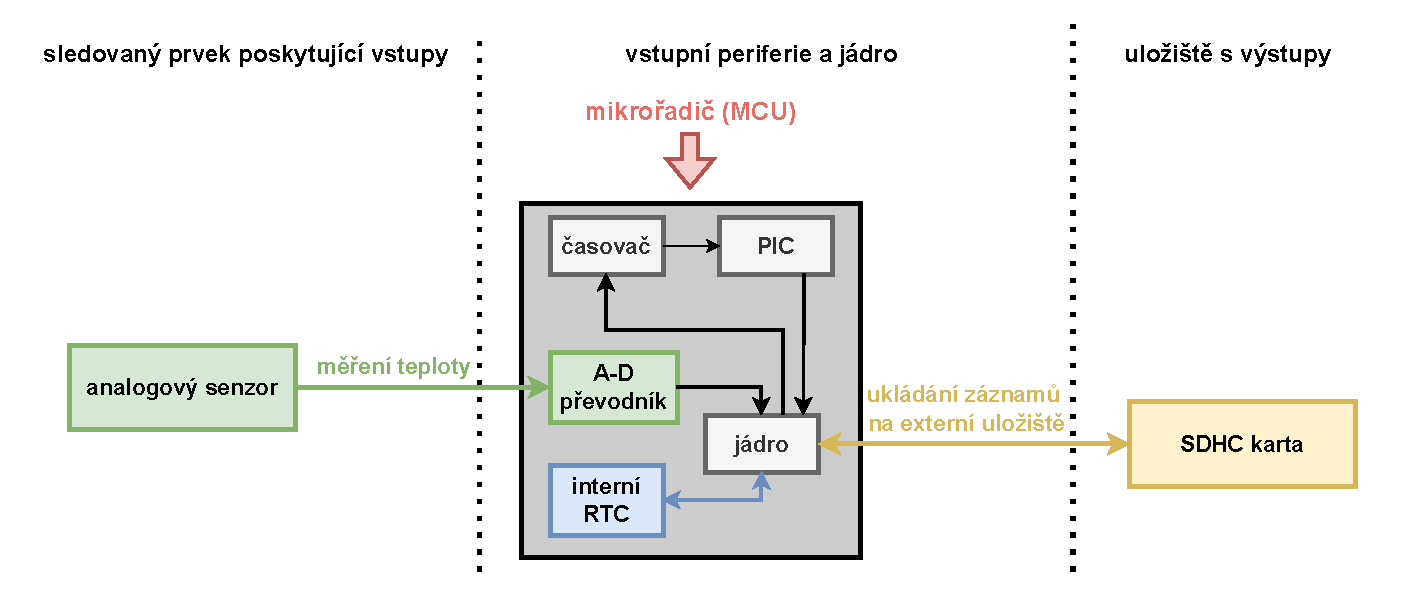
\includegraphics[width=1.00\textwidth]{obrazky-figures/recorder_mcu.pdf}
    
    \caption{Ukázka architektury digitálního záznamníku pro měření teploty}
    \label{fig:mcu-recorder}
\end{figure}

\newpage

Vstupní data jsou následně zpracována jádrem mikrokontroléru, které může provádět základní operace, jako je například převod číslicové hodnoty z ADC na teplotu, filtrování signálu, doplňování časových značek, nebo provádět i obtížnější operace, jako je výpočet tepu v případě měření srdečních aktivit a další výpočty.

Následně jsou digitální data ukládána do paměťového média. Zde lze zvolit obvykle dva přístupy s lokálním a nebo vzdáleným paměťovým uložištěm. Přístup s lokálním paměťovým uložištěm využívá sekundární uložiště, tedy nevolatilní úložiště, která zaručují perzistenci dat i po vypnutí záznamníku. Typickými zástupci těchto pamětí jsou například různé typy SD karet, USB Flash disky a další technologie využívající například technologie NAND a NOR flash paměti. Volatilní paměti, jako je například RAM, se v těchto aplikacích rovněž využívají, avšak výhradně pro krátkodobé uchování dat. V některých případech, například pokud jsou nevolatilní paměti organizovány do bloků (viz. \ref{davkove_zpracovani}), je výhodné nejprve dočasně ukládat data do RAM a teprve po naplnění bloku provést hromadný zápis do nevolatilní paměti, jelikož ukládání do nevolatilních uložišť přináší nové limitace, jakou je například rychlost zápisu,  omezený počet přepisovacích cyklů. Některá úložiště navíc vyžadují mazání celých bloků před opětovným zápisem. Krom lokálního paměťového média je však možné zvolit přístup se vzdáleným uložištěm v podobě databáze či cloudového systému, která však také mají své omezení.


\section{Klíčové koncepty digitálních záznamníku} 
\label{klicove_koncepty_digitalnich_zaznamniku}
Digitální záznamníky mohou být implementovány v podobě dedikovaného zařízení na platformě MCU, dokáží poskytnout dobrý kompromis mezi cenou a výkonem. Na rozdíl od záznamníků realizovaných na výkonnějších platformách, jako jsou osobní počítače nebo jednodeskové počítače, však záznamníky postavené na MCU čelí určitým omezením daným dostupnými hardwarovými prostředky. Proto lze využít některé z optimalizačních technik, zaměřených na vhodnější využití dostupných zdrojů zařízení, které mohou vést k vyššímu výkonu, lepšímu využití dostupného paměťového prostoru nebo například i k lepší spotřebě.

\subsection{Vícenásobná vyrovnávací paměť (multiple-buffering)}
\label{vicenasobna_vyrovnavaci_pamet}
Jedním z častých konceptů využívaných v implementaci digitálních záznamníků je použití vícenásobné vyrovnávací paměti. Tento koncept je převážně známý díky algoritmům využívaným v oboru počítačové grafiky. Grafický čip musí zpracovat velké množství dat za krátký časový úsek, proto algoritmus zpracování dat využívá dvě vyrovnávací paměti, přední vyrovnávací paměť, takzvaný (Front Buffer), jež je využívána pro zobrazení aktuálního snímku, a zadní vyrovnávací paměť (Back Buffer), ve které čip připravuje nový obsah. Jakmile je nový snímek kompletní, vyrovnávací paměti se vzájemně prohodí. Výsledný obsah tak může být plynule vykreslen bez artefaktů a trhání. \cite{double_buffering_model}

Obdobný mechanismus se využívá i v digitálních záznamnících, kde slouží k zajištění kontinuálního sběru dat bez výpadků. Zatímco Back Buffer přijímá nová digitální data ze vstupní periferie a popřípadě je zpracovává, Front Buffer je současně ukládán na úložné médium. Jakmile je Back Buffer naplněn daty a obsah Front Bufferu je uložen, dojde k jejich prohození. Tento algoritmus tak dokáže snížit riziko ztráty dat způsobené časovou prodlevou při jejich zpracování nebo zápisu.

\newpage

\begin{figure}[h]
    \centering
    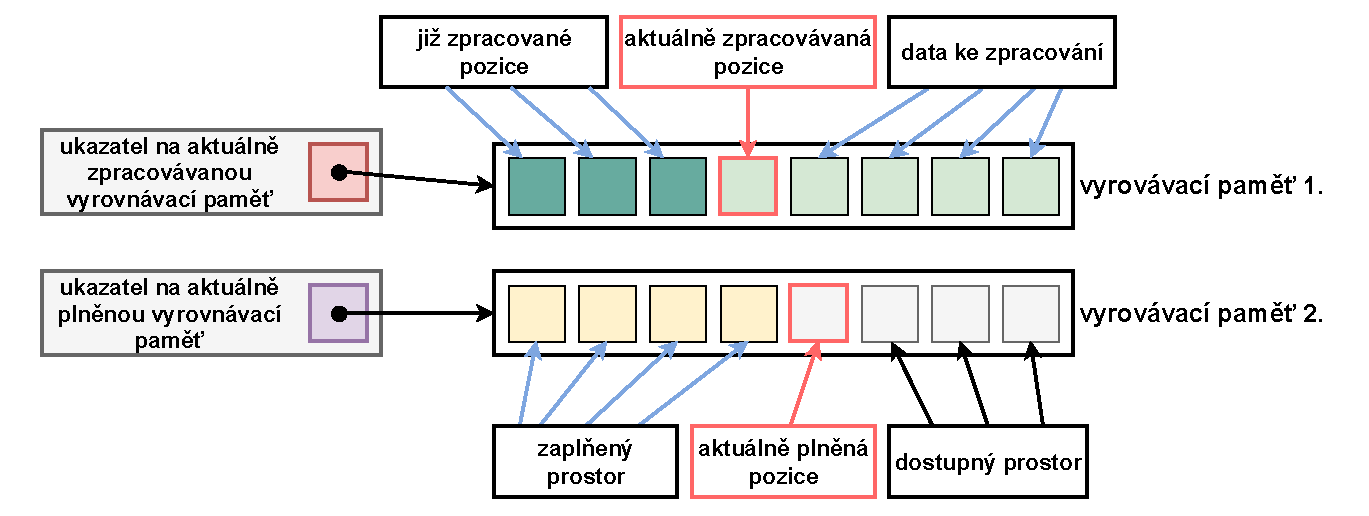
\includegraphics[width=1.00\textwidth]{obrazky-figures/multiple_buffering-1.pdf}
    
    \caption{Schéma principu práce s vícenásobnou vyrovnávací paměťí - náhodný stav}
    \label{fig:multiple-buffering-1}
\end{figure}

% Důležitou vlastností tohoto přístupu je jeho nízká operační režijní náročnost. Plynulý chod zpracování dat je zajištěn bez nutnosti fyzického přenosu obsahu mezi vyrovnávacími pamětmi. Místo toho se využívají ukazatele (pointery), které směřují na počáteční adresy jednotlivých bufferů. Jakmile je Back Buffer naplněn, ukazatele se prohodí, čímž dojde k záměně rolí jednotlivých bufferů, vyrovnávací paměť mající roli Back Buffer je přiřazena role Front Buffer a vyrovnávací paměť s původní rolí Front Buffer je naopak přidělena role Back Buffer.
Důležitou vlastností tohoto přístupu je jeho nízká operační režijní náročnost. Plynulý chod zpracování dat je zajištěn bez nutnosti fyzického přenosu obsahu mezi vyrovnávacími pamětmi. Místo toho se využívají ukazatele (pointery), které směřují na počáteční adresy jednotlivých bufferů. Jakmile je Back Buffer naplněn, ukazatele se prohodí, čímž dojde k záměně rolí jednotlivých bufferů, bufferu mající roli Back Buffer je přiřazena role Front Buffer a naopak bufferu s původní rolí Front Buffer je přidělena role Back Buffer.

\begin{figure}[h]
    \centering
    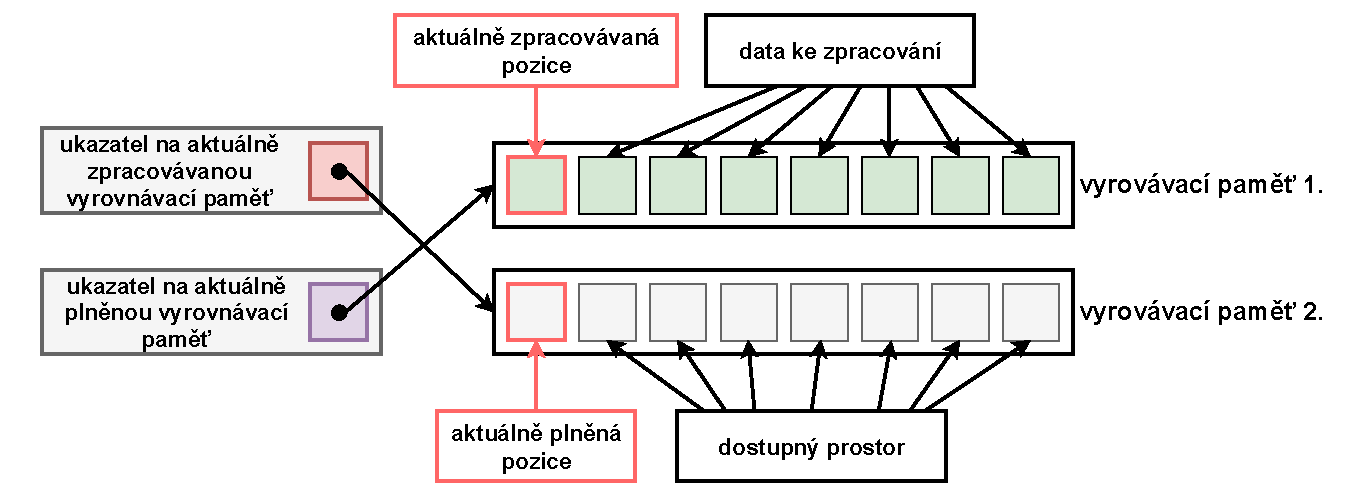
\includegraphics[width=1.00\textwidth]{obrazky-figures/multiple_buffering-2.pdf}
    
    \caption{Schéma principu práce s vícenásobnou vyrovnávací paměťí - přeřazení ukazatelů}
    \label{fig:multiple-buffering-2}
\end{figure}

Tato metoda nachází významné uplatnění zejména v systémech pracujících v reálném čase, kde dochází k příjmu velkého objemu dat v krátkých časových intervalech a kde doba zpracování nesmí překročit dobu sběru dat. Využitím vícenásobné vyrovnávací paměti se minimalizuje latence zpracování a současně se snižuje riziko přetečení paměťového prostoru. Avšak nevýhodou této metody je skutečnost, že vyrovnávací paměti jsou zpravidla implementovány softwarově, nikoliv hardwarově, což vede k zvýšeným nárokům na paměťové prostředky, obzvlášť v segmentu volatilní paměti (RAM) kde jsou buffery často uložené. \cite{buffering_chang, basics_of_digital_forensics}
% TODO: Je tedy vhodne si promyslet zda zdroje MCU budou dostacovat.

\subsection{Dávkové zpracování (batch processing)}
\label{davkove_zpracovani}
Další princip, využívaný v implementacích digitálních záznamníků, souvisí s typem uložišť, na které jsou získaná data zaznamenávána. Data jsou standardně dlouhodobě ukládána na některý z typů nevolatilních pamětí, které umožňují uchování dat i po odpojení napájení. Takovými uložišti jsou například NAND či NOR Flash paměti. Tyto typy paměti jsou organizovány do bloků (popřípadě stránek), přičemž bloky jsou následně rozděleny na menší jednotky zvané sektory. Velikost sektoru obvykle bývá 512 bajtů či 4096 bajtů, v závislosti na typu média a jeho architektuře. Tato bloková struktura umožňuje účinnou správu prostoru, které uložiště nabízí, ale současně vyžaduje specifický způsob zápisu/čtení dat, který je umožněn pouze na úrovni celých sektorů. \cite{tech_target_nand_flash, non_volatile_memories}

Dávkové zpracování tohoto chování paměti využívá, data jsou shromažďována ve volatilní paměti - například RAM, a teprve po naplnění určitého objemu (celého sektoru či jeho násobku) dojde k jejich zápisu na dlouhodobé paměťové médium.

\begin{figure}[h]
    \centering
    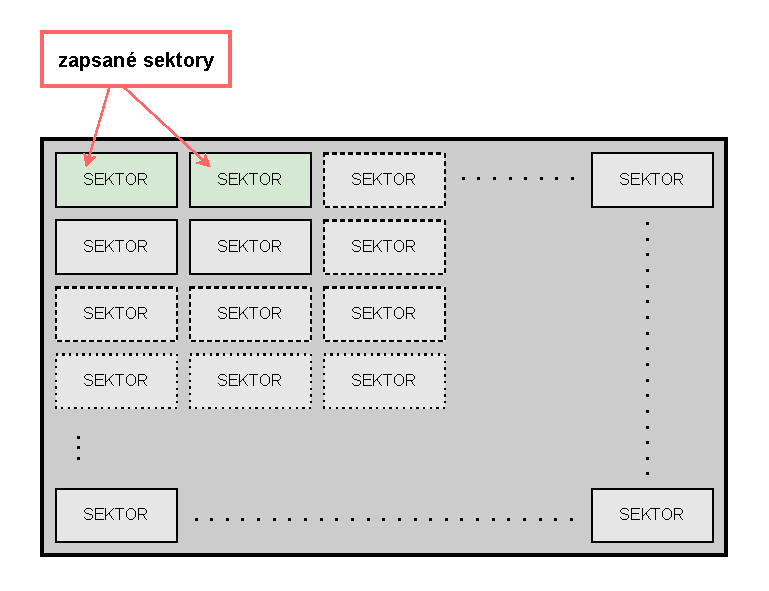
\includegraphics[width=0.75\textwidth]{obrazky-figures/batch_processing.pdf}
    
    \caption{Příklad organizace bloku nevolatilní paměti \cite{ieee_relationships_among_region_segment_frame_and_cluster}}
    \label{fig:batch-processing}
\end{figure}

\newpage

\subsection{Cirkulární buffer}
\label{cirkularni_buffer}
Cirkulární buffer (Circular Buffer), někdy také označovaný jako kruhový nebo cylindrický buffer, je datová struktura, která funguje na principu FIFO fronty (First-In, First-Out) a považuje tuto paměť za kruhovou. Tento přístup je často využíván k řešení problému typu jednoho producenta a konzumenta (Producent-Consumer Problem), kde jedno vlákno je zodpovědné za produkci dat a je tedy producentem, a druhé vlákno je zodpovědné za konzumaci dat. Například ve vestavěných zařízeních, jedním z vláken je rutina obsluhy přerušení, která čte data ze senzoru, a druhým vláknem je hlavní smyčka události, která data nějakým způsobem zpracovává. \cite{embedjournal_ring_buffer}


\begin{figure}[h]
    \centering
    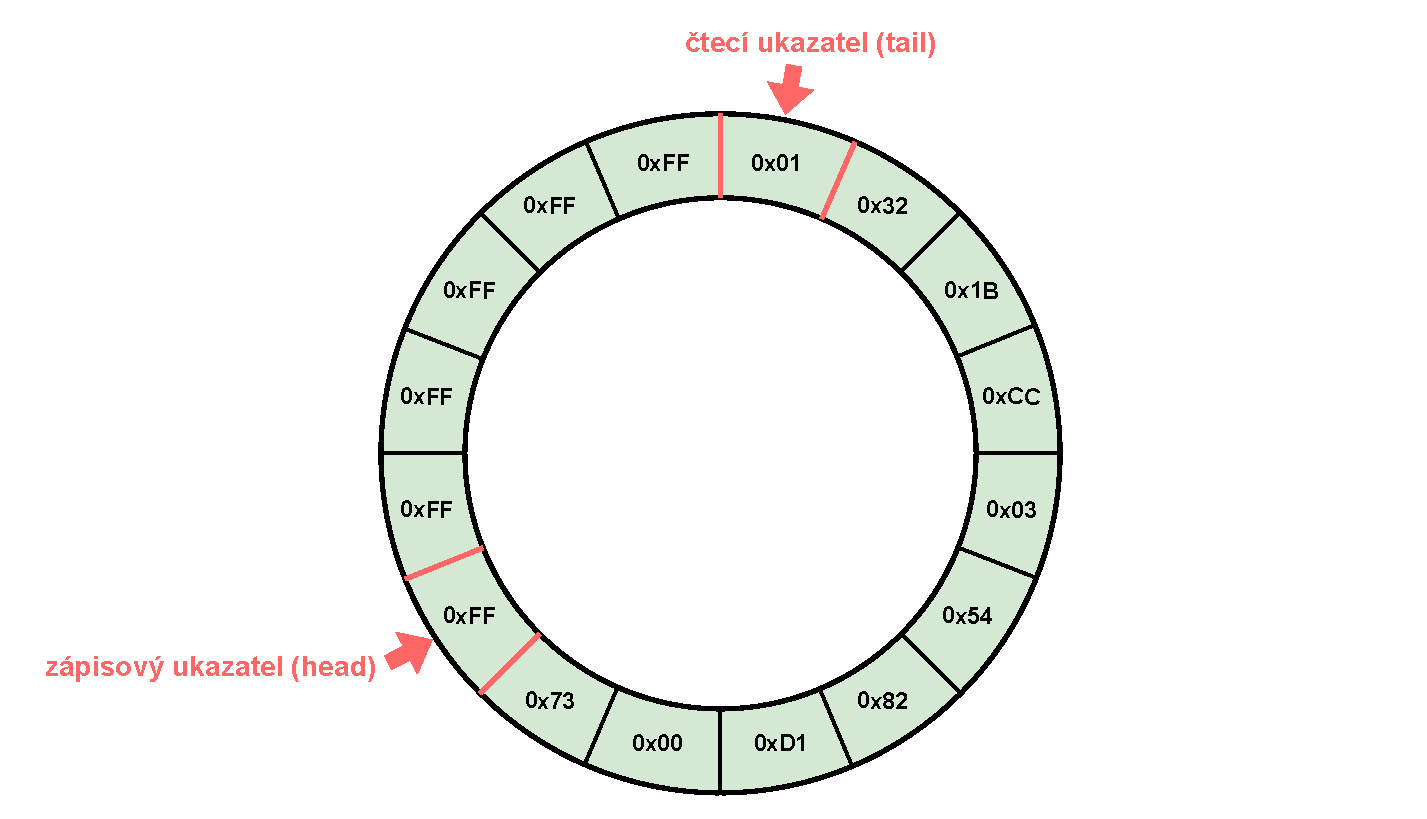
\includegraphics[width=1.00\textwidth]{obrazky-figures/circular_buffer.pdf}
    
    \caption{Cirkulární vyrovnávací paměť}
    \label{fig:circular-buffer}
\end{figure}

Princip činnosti cirkulárního bufferu spočívá v použití dvou ukazatelů - zápisový ukazatel (Head) a čtecí ukazatel (Tail). Ukazatel head vždy směřuje na pozici, kam bude zapisován následující prvek, zatímco ukazatel tail ukazuje na pozici, ze které bude čtena následující hodnota. Pokud ukazatel head dosáhne konce pole, vrací se na jeho začátek, čímž je zajištěna kruhová povaha struktury. Při plném bufferu lze zvolit dvě strategie – přepsání nejstarších dat nebo odmítnutí nových vstupů, přičemž výběr závisí na konkrétní aplikaci. \cite{embedjournal_ring_buffer, medium_ring_buffer}

Z hlediska časové složitosti nabízí cirkulární buffer konstantní časovou složitost $\mathcal{O}(1)$ pro základní operace, jako je zápis (enqueue) a  čtení (dequeue). Tato efektivita je dána tím, že se při zápisu a čtení dat není potřeba přesouvat prvky v paměti, ale lze pouze inkrementovat ukazatele s využitím operace modulo. Pokud jde o prostorovou složitost, velikost cirkulárního bufferu je určena předem – zpravidla jde totiž o staticky alokované, to v tomto případě odpovídá složitosti $\mathcal{O}(n)$, kde $n$ je maximální počet prvků, které může buffer pojmout. \cite{petrungaro_ring_buffer_complexity}

\subsection{Nízko-energetické režimy (Low-Power Modes)}
\label{nizko_energeticke_rezimy}
Energetická efektivita je jedním z klíčových parametrů obecně vestavěných zařízení, tedy i digitálních záznamníků implementovaných na platformě MCU, zejména pokud jsou napájeny z baterií či jiných omezených zdrojů energie (například Energy Harvesting). Minimalizace spotřeby bývá v těchto případech realizována využitím nízkoenergetických režimů (Low-Power Modes), které umožňují zařízení přejít do stavu s minimální energetickou náročností během nečinných period. V praxi mnoho digitálních záznamníků nemusí provádět měření a záznam dat nepřetržitě. Například záznamník teploty může v pravidelných intervalech provést měření, uložit naměřenou hodnotu, přejít do režimu nízké spotřeby a po uplynutí definovaného časového intervalu nebo při výskytu speciální události přejít do aktivního režimu. \cite{analog_devices_low_power_modes}

Průběh takového cyklického chování spotřeby mikrokontroléru, kde se střídají fáze měření a spánku s pravidelnou periodou měření teploty, je znázorněn na obrázku \ref{fig:low-power-modes} níže.

\begin{figure}[h]
    \centering
    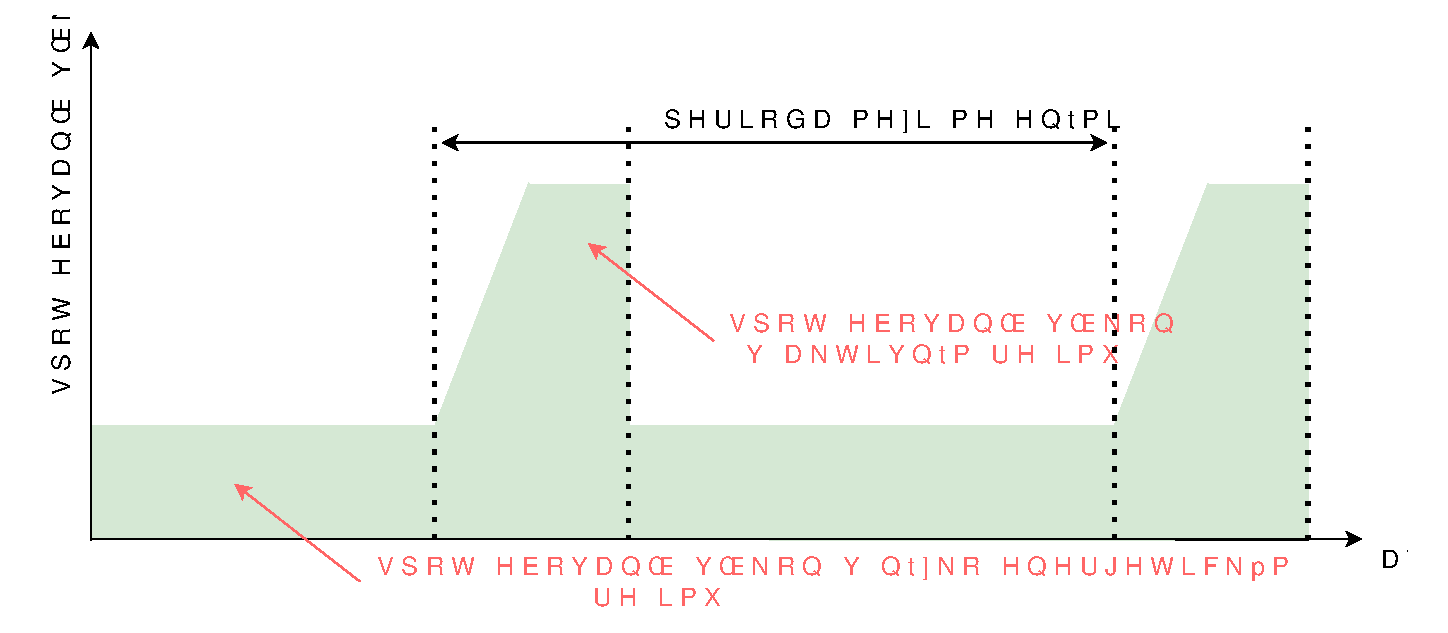
\includegraphics[width=1.00\textwidth]{obrazky-figures/low_power_modes-cz.pdf}
    
    \caption{Graf znázorňujíci dynamiku spotřeby mikrokontroléru v průběhu času při využití aktivního a nízkoenergetického režimu}
    \label{fig:low-power-modes}
\end{figure}

Ačkoliv nízkoenergetické režimy přinášejí značné úspory energie a jsou nezbytné pro zařízení napájená z baterií, u dataloggerů s velkým objemem zaznamenávaných dat mohou představovat významná omezení. Tyto režimy sice snižují energetickou náročnost systému, avšak zároveň omezují schopnost mikrokontroléru rychle reagovat na události. Spánkové stavy, které minimalizují spotřebu energie, často vedou k delšímu zpoždění při probuzení a nižší dostupnosti kritických periferií. V aplikacích, kde je vyžadována okamžitá odezva na externí podněty nebo nepřetržité zpracování velkého množství dat, může tento faktor negativně ovlivnit spolehlivost a efektivitu záznamníku. \cite{embedded_low_power_modes}

V těchto případech je proto nutné zvážit provozní podmínky a očekávanou dostupnost systému. Pokud záznamník pracuje s velkým datovým tokem a má možnost být připojen po dobu záznamu stále k externímu napájení, může být výhodnější upustit od implementace nízkoenergetických režimů a místo toho optimalizovat architekturu systému pro nepřetržitý provoz s důrazem na výkon a rychlou odezvu. \cite{analog_devices_low_power_modes}

% Normostrany = 11.34

% Moznosti zapisu dat
\section{Způsoby zápisu dat}
Podobně jako jsou podstatné uložiště, na které jsou zaznamenaná data zapsána, je také důležitá práce s tímto uložištěm. Záznamníky dat musí být navrženy tak, aby umožnily spolehlivé ukládání získaných dat, které by mělo být efektivní ve smyslu rychlosti a šetrné pro zvýšení životnosti uložiště. V této kapitole jsou popsány tři různé způsoby ukládání dat, přímý zápis na lokální úložiště, ukládání prostřednictvím mezivrstvy s FRAM pamětí a využití vzdálených úložišť. Každá z těchto metod má své specifické výhody a omezení, které určují její vhodnost pro konkrétní aplikace.

\subsection{Přímý zápis na permanentní uložiště}
Přímý zápis na permanentní úložiště představuje nejjednodušší a nejpřímější metodu ukládání dat. V tomto případě jsou zaznamenaná data ihned zapisována na nevolatilní paměťové médium, jako je SD karta, eMMC, USB Flash disk nebo NAND Flash čip. Tento způsob eliminuje potřebu mezivrstvy mezi záznamníkem a úložištěm, čímž se minimalizuje latence a zjednodušuje celková implementace.

\begin{figure}[h]
    \centering
    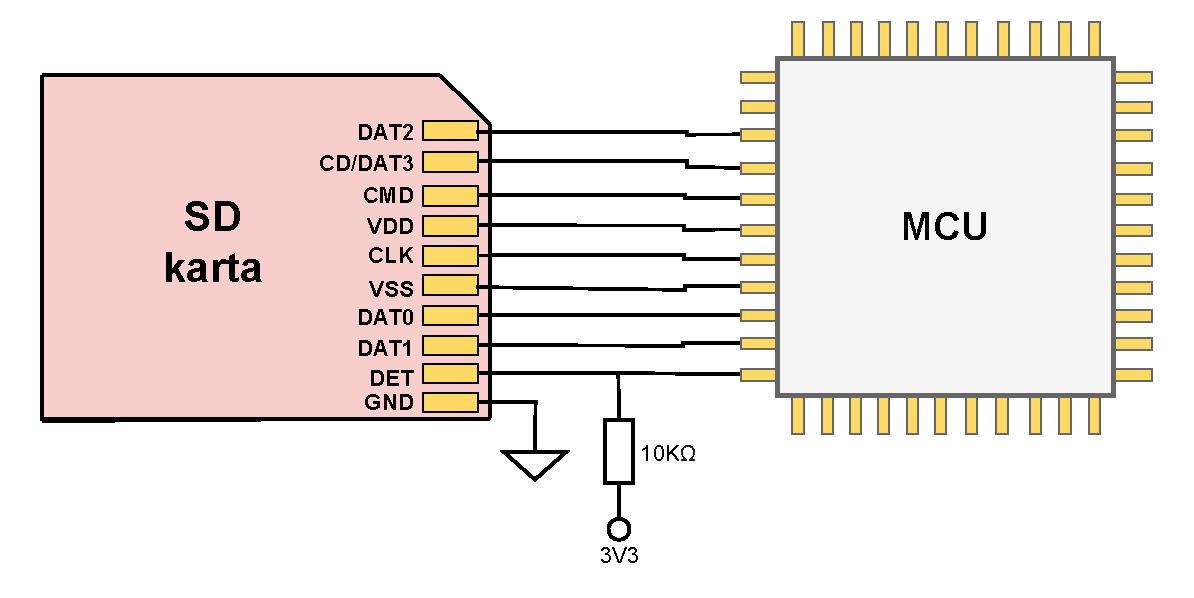
\includegraphics[width=1.00\textwidth]{obrazky-figures/forward_write.pdf}
    
    \caption{Přímý zápis na permanentní uložiště s SDHC kartou za pomocí čtyř pinové datové sběrnice}
    \label{fig:forward-write}
\end{figure}

Hlavní výhodou této metody je její jednoduchost a okamžitá perzistence dat. Data jsou ukládána přímo na trvalé úložiště a nehrozí tak jejich ztráta při výpadku napájení. To je zvláště výhodné v záznamnících, které zapisují drobné množství dat, kde se data neměří neustále, ale jednou za danou periodu uvedenou v kapitole \ref{nizko_energeticke_rezimy}, například v environmentálních záznamnících monitorujících teplotu nebo vlhkost.

Problémem tohoto principu je však častý zápis na paměťové médium. Proto, aby se předešlo nadměrnému opotřebení uložiště a zvýšila se efektivita zápisu, využívá se mnohdy současně metoda dávkového zpracování (Batch Processing), která již byla zmíněná v kapitole \ref{davkove_zpracovani}. Data jsou krátkodobě uložena ve volatilním uložišti, a jakmile jich je nashromážděno dostatek, tak jsou přepsána do dlouhodobé nevolatilní paměti. To ale přináší i nové problémy, kdy hodnoty uložené v neperzistentním uložišti jsou vystavena riziku ztráty v případě ztráty napájecího napětí.

\subsection{Zápis na permanentní uložiště přes mezivrstvu s FRAM paměti}
Alternativní volbou k přímému zápisu na permanentní úložiště je využití mezivrstvy ve formě FRAM (Ferroelectric Random Access Memory). FRAM je nevolatilní paměť, jež kombinuje výhody rychlé volatilní RAM paměti a perzistentního úložiště.

Ve feroelektrické RAM paměti (FRAM/FeRAM) jsou data ukládána pomocí změny polarizace feroelektrického materiálu v paměťové buňce. Jednotlivé buňky se skládají podobně jako je tomu u dynamické RAM (DRAM), z jednoho tranzistoru a jednoho feroelektrického kondenzátoru (1T-1C). Na rozdíl však od DRAM, kde je informace uchovávána jako elektrický náboj v lineárním dielektriku, FeRAM využívá feroelektrický materiál, jakým je třeba titaničitan olovnatý (PZT), který vykazuje hysterezní chování. Jakmile je aktivní elektrické pole, dipóly se v krystalové mřížce přeuspořádají do jednoho ze dvou stabilních stavů odpovídajících binárním hodnotám nula či jedna a tento stav zůstává zachován i po odeznění elektrického pole. K samotnému čtení a zápisu do konkrétní paměťové buňky jsou využívány tři hlavní signálové linky Word Line a Bit Line určující konkrétní buňku a Plate Line, která vytváří elektrické pole potřebné k přepólování feroelektrického materiálu během zápisu. \cite{ieee_feram_ultra_high_density_embedded_mem}

\begin{figure}[h]
    \centering
    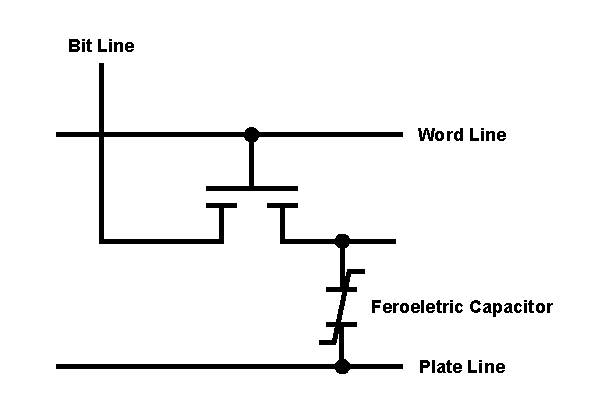
\includegraphics[width=0.70\textwidth]{obrazky-figures/fram_t1-c1.pdf}
    
    \caption{Struktura 1T-1C feroelektrické RAM paměti (FeRAM) \cite{researchgate_nonvolatile_memory_technologies}}
    \label{fig:feram-1t-1c}
\end{figure}
% Word Line - slovni linka, pomoci ni se aktivuje pristup k jednomu radku bunek, aktivuje se pri cteni ci zapisu konkretniho slova ci bajtu 
% Word Line 
% Bit Line - bitova linka, vertikalni spojeni pametovych bunek, kazdy sloupec ma svoji bitovou linku
% Plate Line - použita k vytvoření elektrického pole, které umožňuje přepólování feroelektrického materiálu

FRAM lze v dedikovaném digitálním záznamníku využít jako takzvanou mezivrstvu neboli vyrovnávací paměť, pomocí které lze optimalizovat zápisy na konečné dlouhodobé úložiště. Jak jsou tedy data záznamníkem postupně sbírána, tak mohou být postupně či po blocích zapisována do této mezivrstvy. Pokud je následně vyrovnávací paměť FRAM dostatečně zaplněna, její obsah je dávkově přenesen na dohodnuté trvalé úložiště, a tento cyklus se opakuje. 


Nevýhodou tohoto přístupu může být vyšší režie v případech, kdy digitální záznamník využívá souborový systém a jako úložiště SD kartu. Digitální záznamník totiž nejprve musí přijatá data zpracovat, tj. doplnit časové značky, tedy i tak je potřeba mít nějaký buffer v RAM, zpracovaná data by pak byla přesunuta z RAM do FeRAM, kde by byla dočasně uchována, a následně opět načtena zpět do RAM, aby mohla být zapsána do souboru na SD kartu. Ve výsledku by tedy i tento přístup vyžadoval dostatečně velký buffer v RAM, a tím by se výhoda použití FeRAM jako mezivrstvy do značné míry ztratila.

% navíc nevolatilní, diky usporadanym dipolum, ktere bylo zajisteno aktivnim elektrickem poli 
Použití FRAM jako vyrovnávací paměti přináší několik výhod. Jedním z hlavních přínosů je snížení opotřebení hlavního úložiště, eliminován je totiž častý zápis po malých blocích dat, který zbytečně opotřebovává koncová nevolatilní úložiště typu flash, která mají omezený počet přepisovacích cyklů. Další výhodou je velice rychlý zápis oproti flash pamětem, obvykle trvá zápis na FRAM v řádu nanosekund, což je řádově rychlejší než srovnávané flash paměti, na kterých zápis trvá typicky v řádu mikrosekund až milisekund. FRAM je navíc nevolatilní, což znamená, že i v případě výpadku napájecího napětí zůstávají zaznamenaná data na feroelektrickém uložišti zachována, čímž se eliminuje potřeba dodatečných opatření k ochraně dat, jako jsou záložní baterie nebo superkondenzátory.

\subsection{Zápis na vzdálené uložiště}
\label{zapis_na_vzdalene_uloziste}
Pro dlouhodobé uložení dat lze také využít vzdálená uložiště, jakými jsou databáze či cloudy. Lze tak využít jednotného uložiště pro velké množství digitálních záznamníků a eliminovat tak potřebu lokálních, nevolatilních paměťových médií. Zmiňované jednotné uložiště může být jak centrální server, tak i distribuovaná síťová soustava, umožňující uložení daleko většího množství dat, než může nabídnout lokální uložiště.

% Neni to tak ze CoAP a MQTT jsou si rovny, MQTT se hodi spis na komunikaci, kde Tx a Rx jsou synchronizovany, kde komunikace probiha casto asynchronne, jedno zarizeni data vysila a ostatni je mohou odebirat a nasledne prijimat, takhle jde udelat efektivni komunikaci bez nutnosti synchronizace
% CoAP, je zase spis pro format dotaz-odpoved mimikuje HTTP
V praxi dedikovaný záznamník, který data buď přímo zpracovává, nebo je dočasně uchovává ve volatilní paměti, využívá síťové rozhraní k jejich přenosu do vzdáleného úložiště. Přenos probíhá obvykle prostřednictvím aplikačních síťových protokolů postavených nad transportním protokolem TCP (Transmission Control Protocol), jakým je MQTT, nebo nad protokolem UDP, nad kterým je postaven třeba protokol CoAP. Každý z uvedených zástupců poskytuje trošku odlišnou funkcionalitu. MQTT je vhodnější pro komunikaci, kde odesílatel a příjemce nejsou synchronizováni a dialog probíhá asynchronně. Vysílatel tedy odesílá data a ostatní zařízení tato data mohou začít přijímat. Zato CoAP zase prosazuje formát komunikace typu dotaz-odpověď, kterým mimikuje HTTP. \cite{emq_mqtt_vs_coap}


\begin{figure}[h]
    \centering
    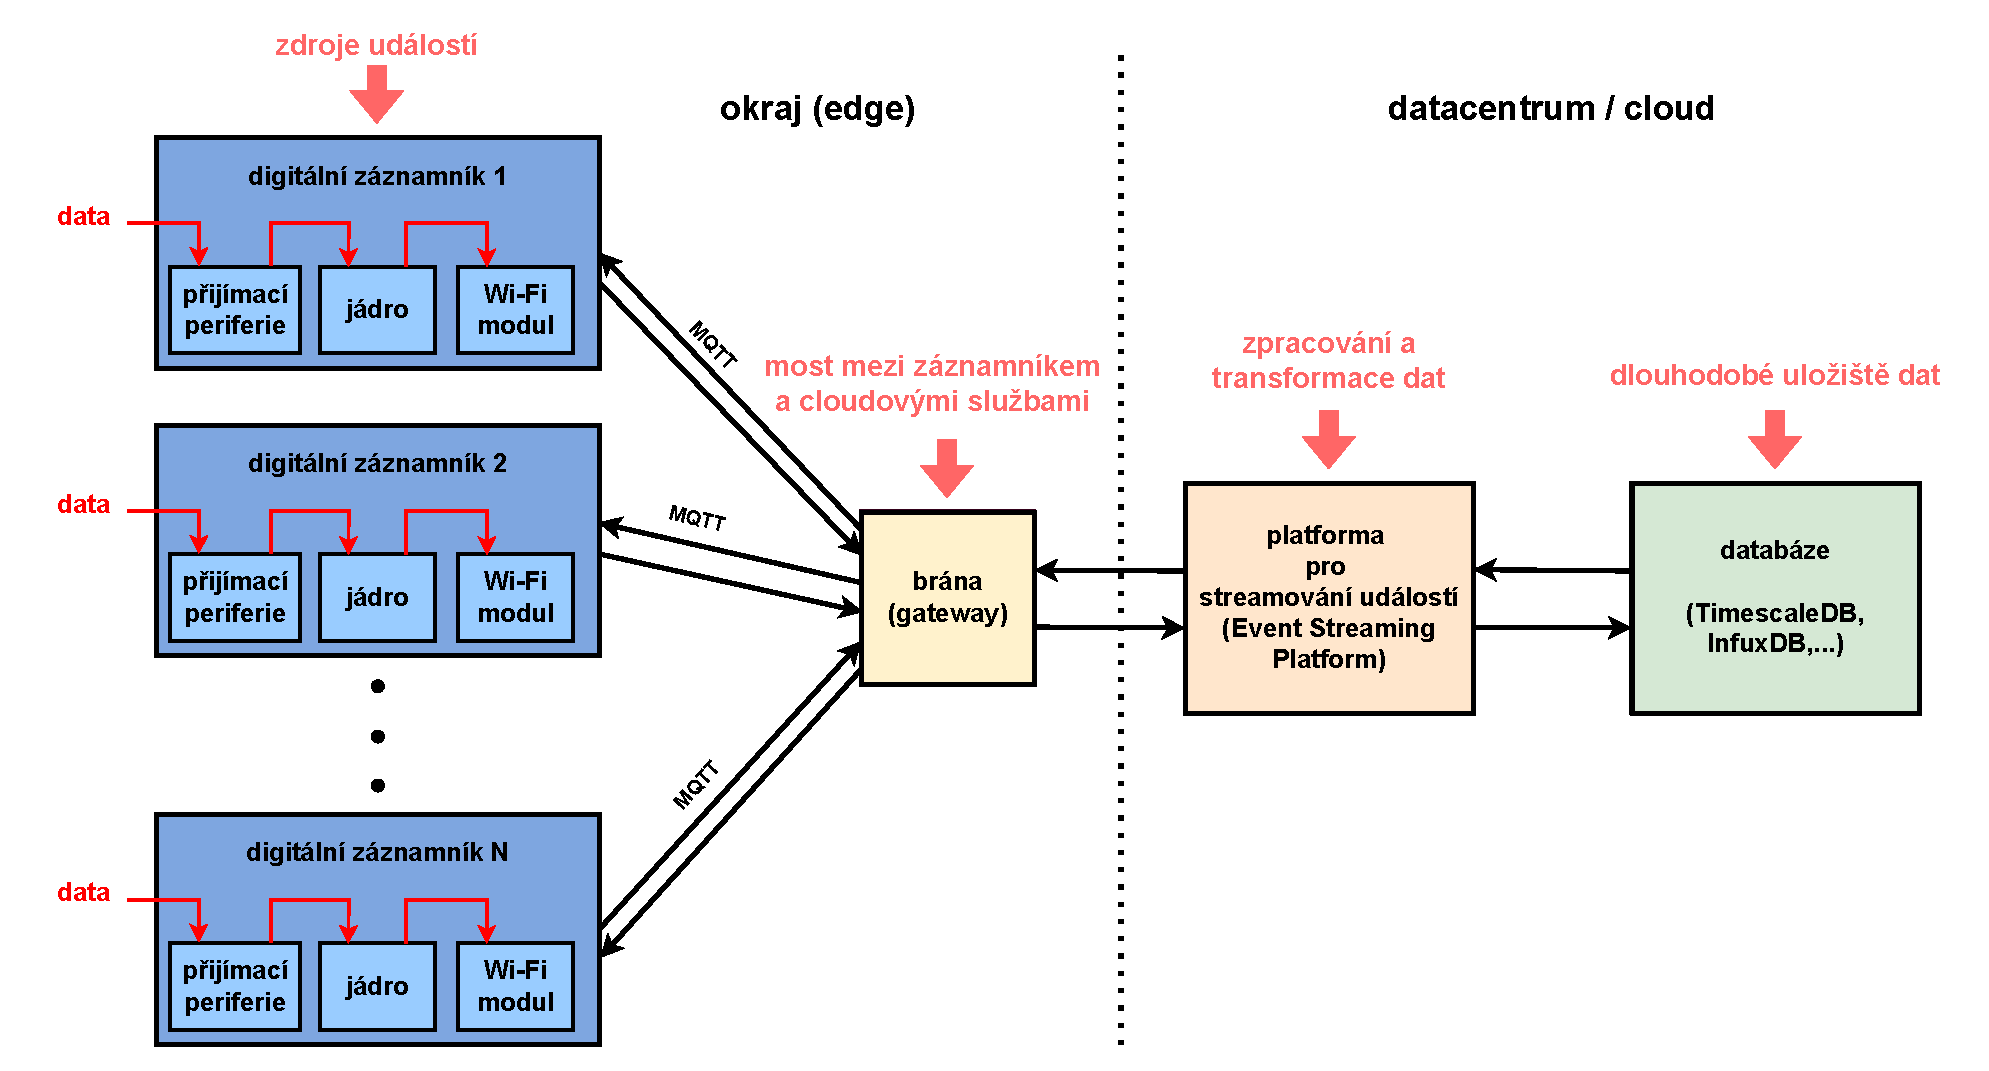
\includegraphics[width=1.00\textwidth]{obrazky-figures/advanced_architecture_of_datalogging.pdf}
    
    \caption{Schéma pokročilého digitálního záznamníkíku s cloudovým uložištěm postavený na streamingové platformě Kafka \cite{confluent_advanced_datalogging, influxdata_advanced_datalogging_mmqt}}
    \label{fig:advanced-architecture-of-datalogging}
\end{figure}

% Pouzivaji se treba v pokrocilych systemech kdy uz je mozne z dat neco i odvozovat, napriklad venku je pekne a v dobe je 25 stupnu tak trosku pootevru okna.

Následně jsou data ukládána na již zmiňované databázové servery či cloudové služby. Databázové servery mohou být postaveny na různých technologiích v závislosti na typu dat a požadavcích na jejich zpracování. Často jsou využívány systémy, které umožňují pracovat s daty ve formátu časových řad, což jsou sekvence datových bodů zaznamenávaných ať už v pravidelných či nepravidelných časových intervalech. Na taková data může být tedy vhodné využít například InfluxDB nebo TimescaleDB.\footnote{Možné je také zvolit relační databáze, ale ty jsou u digitální záznamníků méně časté.} Cloudová řešení jsou pak objektová uložiště, kde jsou data ukládána v podobě souborů či binárních objektů. Zároveň tyto služby umožňují krom samotného uložení přidat i analytickou vrstvu, která umožňuje zpracování dat v reálném čase a reagovat tak na aktuální stav. K tomuto účelu pak lze využít třeba streamovací platformy, jakými jsou Apache Kafka (viz. obrázek \ref{fig:advanced-architecture-of-datalogging} a AWS Kinesis. \cite{springer_analysis_time_series_db_edge_computing}

Výhodou tohoto přístupu je především možnost centralizovaného ukládání a zpracování dat, to se hodí při velkých množstvích digitálních záznamníků, jelikož v takovémto případě je obtížné manuálně kontrolovat všechna zařízení a postupně z nich extrahovat získaná data. Další výhodou je schopnost systému reagovat na aktuální stav prostředí nebo na základě dat odvozovat vhodná opatření. Tento princip lze efektivně využít například v chytrých domácnostech nebo průmyslových provozech, kde lze automaticky upravovat provoz zařízení, jako je klimatizace, vytápění či osvětlení, na základě hodnot získaných ze senzorů. \cite{springer_analysis_time_series_db_edge_computing}

Tento přístup se hodí pro digitální záznamníky operující ve známých prostředích, kterým je třeba zmiňovaná chytrá domácnost či továrna, jelikož je potřeba zaručit stabilní připojení k síti. Pokud by měl záznamník cestovat různě po světě, bylo by nutné jej na každém novém místě připojit k Wi-Fi síti či Ethernetu, nebo by jej bylo nutné koncipovat jako digitální záznamník se SIM kartou, pomocí které by byl zajištěn přístup k mobilní síti. Dále je důležité mít i koncipovanou komplexní infrastrukturu, v níž je zajištěn bezpečný přenos dat. Pro tento síťový přenos je třeba přidat další úroveň zabezpečení, která zajistí autentizaci, šifrování, integritu dat a případně další bezpečnostní prvky. S bezpečností souvisí také nezbytnost, aby zařízení poskytovalo zdroje pro běh plnohodnotného TCP/IP modulu
(stack), díky kterému bude možné využít bezpečnostní prvky jako je například SSL/TLS a který je zároveň potřebný pro již zmíněný protokol MQTT, běžící nad transportním protokolem TCP.


\chapter{Návrh digitálního záznamníku}
\label{navrh_digitalniho_zaznamniku}

\section{Existující řešení digitálních záznamníku}
Jak již bylo zmíněno v předchozích kapitolách, problematika záznamu dat provází lidstvo od nepaměti. Stejně tak samotné záznamníky dat nejsou novým tématem a v praxi již existuje celá řada produkčních řešení zaměřených na záznam různých typů dat. Tato kapitola je věnována popisu některých dostupných řešení, konkrétně záznamníkům zaměřeným na záznam datových toků zmíněných v kapitole \ref{digitalni_zaznam_dat}, mezi které se bude řadit i výsledné zařízení, které jsem navrhl, implementoval a popsal v této bakalářské práci. 


\subsection{OpenLog Serial Data Logger}
\label{openlog_serial_datalogger_module}
Prvním z vybraných existujících záznamníků je modul OpenLog, který je kompaktní a snadno použitelné zařízení pro záznam sériové komunikace, který vyvinula společnost SparkFun. Tento záznamník běží na osmibitovém mikrokontroléru ATmega328P taktovaném na 16 MHz a je navržen tak, aby umožnil přímý záznam sériové komunikace na microSD kartu s podporou až do velikosti 32 GB a bez nutnosti složitější konfigurace. \cite{sparkfun_openlog_tutorial}

\begin{figure}[h]
    \centering
    \includegraphics[width=0.85\textwidth]{obrazky-figures/sparkfun-openlog.png}
    
    \caption{Digitální záznamník SparkFun Openlog \cite{cirkit_openlog}}
    \label{fig:sparkfun-openlog}
\end{figure}

Tento záznamník je vhodný na jednoduché projekty, hobby projekty, či prototypování, záznamník OpenLog lze totiž snadno použít v systémech postavených například na nepájivém poli. Záznamník je vhodný k monitorování systémů, které již provedly předzpracování dat ze svých datových zdrojů a potřebují data jen uložit (viz. obrázek \ref{fig:sparkfun-openlog-use-case}). Obvykle je v tomto případě hlavní mikrokontrolér, který přijímá monitorovaná data (např. z GPS modulu) a následně je jakýmsi způsobem zpracovává a formátuje do koncové podoby a následně je posílá po sériové lince na bázi UART komunikace do Openlog modulu. Záznamník si data následně ukládá do vyrovnávací paměti ve volatilní RAM paměti a jakmile se tento buffer naplní (viz. kapitola \ref{davkove_zpracovani}), tedy Openlog nasbírá 512 bajtů, tak je zapíše do micro SD karty. \cite{cirkit_openlog}

\begin{figure}[h]
    \centering
    \includegraphics[width=0.85\textwidth]{obrazky-figures/sparkfun-openlog-use-case.png}
    
    \caption{Sledovací zařízení GPS se záznamem dat \cite{cirkit_openlog}}
    \label{fig:sparkfun-openlog-use-case}
\end{figure}

Nevýhodou tohoto záznamníku je, že hlavní mikrokontrolér, který zpracovává data a posílá data následně do záznamníků, musí být aplikačně předchystán k tomuto účelu, což zvyšuje režii (overhead) navíc. Řídící MCU musí buď pomocí příkazů nastavit parametry záznamu, jako je baudrate, vytvoření souboru, přidání dat do souboru a další funkcionality, nebo je třeba využít konfigurační soubor uložený na SD kartě. Bohužel po nastavení v konfiguračním souboru je nutné provést restart záznamníku, než se provede aktualizace nastavení. Záznamník podporuje zápis na SD karty s kapacitou od 64 MB do 32 GB se souborovými systémy, nicméně je nutné tuto SD kartu zformátovat na zařízeních s operačním systémem Windows. Další nevýhodou tohoto záznamníku je, že nepodporuje přístup na SD kartu bez nutnosti vyjmutí fyzického uložiště.

\subsection{Keeylog AirDrive Serial Logger}
\label{keelog_airdrive_serial_datalogger}
Dalším řešením digitálního záznamníku je AirDrive Serial Logger, vyvinutý společností Keelog. Zařízení AirDrive je moderní digitální záznamník poskytující bezdrátový přístup k datům, který umožňuje záznam sériových dat pomocí komunikačního standardu RS-232 či RS-485. Na rozdíl od tradičních řešení, která ukládají data pouze na lokální úložiště, nabízí tento záznamník konektivitu k Wi-Fi síti, čímž umožňuje vzdálený přístup k uloženým datům bez nutnosti vyjmutí fyzického média a manipulace s tímto zařízením. Společnost Keelog poskytuje vícero variant AirDrive záznamníků, které se liší poskytnutými funkcionalitami. Hlavním rozdílem mezi jednotlivými verzemi je odlišný přístup k získaným datům, základní verze pracuje jako Wi-Fi hotspot, zatímco verze Pro a Max umožňují připojení do existující Wi-Fi sítě a také odesílání e-mailových reportů, časové razítkování záznamů nebo dokonce živé streamování dat. V čem se naopak zmíněné verze neliší, je velikostí interní paměti, která činí 16 GB, jež je uživatelsky přístupná i jako USB flash disk s rychlostí až 480 Mbps. Zařízení jako AirDrive nachází uplatnění zejména v průmyslovém monitorování, zpětném inženýrství sériových protokolů, zálohování dat z platebních terminálů nebo sběru dat ze senzorových systémů. \cite{keelog_airdrive_serial_datalogger, keelog_airdrive_serial_datalogger_max, keelog_airdrive_serial_datalogger_pro}

\begin{figure}[h]
    \centering
    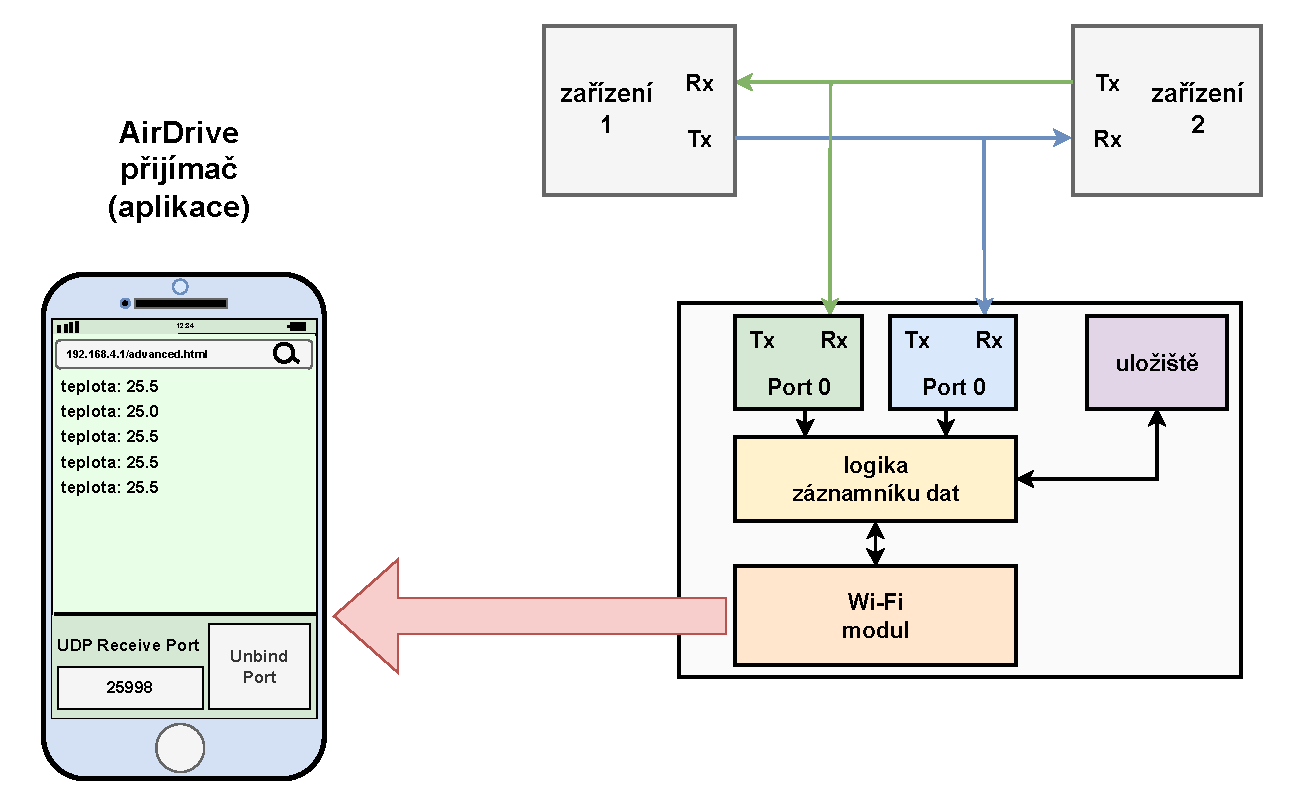
\includegraphics[width=0.90\textwidth]{obrazky-figures/keeylog_airdrive_serial_logger-cz.pdf}
    
    \caption{Keeylog AirDrive Serial Logger s přístupem k datům přes webové rozhraní \cite{keelog_airdrive_serial_datalogger, keelog_airdrive_serial_datalogger_scheme}}
    \label{fig:keelog-airdrive-serial-datalogger}
\end{figure}

Hlavní výhodou AirDrive Serial Loggeru je již zmiňovaná poskytovaná bezdrátová konektivita, která umožňuje přístup k datům z jakéhokoliv zařízení s Wi-Fi připojením, což se může hodit zejména v průmyslových  prostředích, kde může být velký počet takovýchto zařízení a získaná data tak mohou být hromaděna na jednom místě. Tímto centrálním bodem může být například cloudové úložiště nebo serverová databáze (viz. kapitola \ref{zapis_na_vzdalene_uloziste}), kam mohou být data pravidelně odesílána a následně mohou být analyzována. Tento záznamník také podporuje možnost konfigurace pomocí souboru CONFIG.TXT, ve kterém je možné nastavit, s jakou frekvencí budou získaná data odesílána do koncového úložiště. Pro a Max verze umožňují také nastavit tzv. živé vysílání (live streaming), při němž data mohou být monitorována a analyzována v reálném čase. Možné je také k datům přiřazovat časová razítka (timestamps), to se může hodit pro monitorování systémů, jejichž chování se chystáme porovnávat vůči jiným systémům a je tedy nutné si synchronizovat dva záznamy z různých zařízení. \cite{keelog_airdrive_serial_datalogger}

Navzdory svým pokročilým funkcím má AirDrive Serial Logger i několik nevýhod. Jednou z nich je omezení na standardy RS-232 a RS-485, které sice stále nacházejí uplatnění v průmyslových a v řadě dalších systémů, avšak v některých ostatních zařízeních je pro připojení k jiným rozhraním nutné využít sériové převodníky. Jelikož tyto standardy využívají asynchronní sériovou komunikaci (UART), není možné s tímto záznamníkem přímo zaznamenávat data z jiných běžných komunikačních sběrnic, jako jsou I\textsuperscript{2}C, SPI, USB, CAN a také nepodporuje možnost digitalizace pomocí A-D převodníku. Tím se omezuje jeho univerzálnost a možnost použití v širším spektru aplikací. Další limitací je maximální přijímací přenosová rychlost UART (baud rate), která dosahuje pouze 115200 bps. To je například nevyhovující pro monitorování systémů bezdrátového nabíjení společnosti NXP Semiconductors, kde se komunikace probíhá s vyšší komunikační rychlostí. \cite{keelog_airdrive_serial_datalogger}

\subsection{Anticyclone Systems AntiLog Data Logger Pro}
\label{anticyclone_systems_antilog_data_logger}
Posledním zmíněným řešením digitálního záznamníku je AntiLog Data Logger od společnosti Anticyclone Systems, který lze klasifikovat jako vysoce výkonný digitální záznamník určený pro záznam sériových dat v průmyslových a vývojových aplikacích.\footnote{Společnost Anticyclone Systems nabízí tři varianty těchto záznamníků, v tomto textu je primárně popsána verze Pro, jež je svými parametry a funkcionalitou nejblíže záznamníkům, které jsou předmětem této bakalářské práce.} Podobně jako u řešení od společnosti Keeylog (viz. kapitola \ref{keelog_airdrive_serial_datalogger}) umožňuje data přijímat pomocí standardu RS-232 a také plnohodnotně zaznamenávat obousměrné sériové přenosy s vysokými přenosovými rychlostmi až 921 600 baudů. Zařízení umožňuje dlouhodobé zaznamenávání díky podpoře velkokapacitních nevolatilních úložišť až do velikosti 1 TB. Datalogger existuje v několika provedeních - verze AntiLog, AntiLog Pro a také OEM verze (ta je ve formě modulu), která umožňuje přímou integraci do jiných systémů. Nejpokročilejší verze Pro podporuje funkce jako časové razítkování (timestamps), podpora GNSS/NMEA dat a možnost vícekanálového záznamu, což jej činí vhodnou volbou pro aplikace, kde je potřeba přesné a rozsáhlé monitorování sériových přenosů. \cite{anticyclone_systems_antilog_pro}

\begin{figure}[h]
    \centering
    \includegraphics[width=0.6\textwidth]{obrazky-figures/antilogpro.png}
    
    \caption{Anticyclone Anti-Log Pro \cite{anticyclone_systems_antilog_pro_price}}
    \label{fig:antilog-pro}
\end{figure}

Hlavní výhodou AntiLog Pro záznamníku je podpora vysokých přenosových rychlostí, což umožňuje záznam širokého spektra zařízení, která společně s nízkou spotřebou a možností přípojení baterie umožňují použití jak ve vnitřních prostředích, tak i v exteriérech, tedy například v přírodě. Záznamník podporuje pokročilé časové razítkování (timestamping) s rezolucí až jednu milisekundu, usnadňující synchronizaci a post-processing dat. Záznam lze rozšířit o měření veličin, jako je teplota, vlhkost či tlak, prostřednictvím podporovaných senzorů komunikujících po sběrnici I\textsuperscript{2}C, a to paralelně se záznamem až dvou datových kanálů využívajících standard RS-232. Možné je také propojení až 255 jednotek do jednoho vícekanálového záznamníku, které pak umožňuje komplexní monitorování více zařízení současně. \cite{anticyclone_systems_antilog_pro, anticyclone_systems_antilog_pro_extended_logging}

Přesto má AntiLog Data Logger i své nevýhody. Velkým omezením je vysoká pořizovací cena, ta se aktuálně pohybuje u zařízení Anticyclone Anti-Log Pro od 229 £ do 366 £. Pro konfiguraci a přehrávání zaznamenaných dat je také nutné využívat speciální aplikaci AntiTermPro RS-232 terminálový software, což znesnadňuje práci se zařízením pro nezkušenou obsluhu.  \cite{anticyclone_systems_antilog_pro, anticyclone_systems_antilog_pro_price}

\subsection{Shrnutí představených řešení}

Představená existující řešení reprezentují různé přístupy k problematice digitálního záznamu sériových dat, ať už se jedná o jednoduché a cenově velmi dostupné systémy typu OpenLog, pokročilejší řešení, jakými je  AirDrive Serial Logger a AntiLog Pro. Každé z těchto řešení má své výhody, od kapacity úložiště přes různé možnosti přístupu k získaným datům až po vysokou přenosovou rychlost a další vlastnosti zmíněné v kapitolách věnujících se jednotlivým zařízením.

Navzdory těmto vlastnostem však žádné z uvedených řešení plně neodpovídá požadavkům pro záznam dat společnosti NXP Semiconductors. Požadovaný digitální záznamník musí zvládat zaznamenávat sériovou komunikaci o rychlosti mezi 230,000-400,000 baudů, dále je potřeba vkládat časová razítka (timestamps), jelikož výsledné záznamy musí být možné synchronizovat s dalším systémem. Nezbytně nutné je, aby záznamník disponoval mechanismem prevence proti ztrátě dat při výpadku napájecího napětí, získaná data musí být možné vyčíst bez nutnosti vyjmutí fyzického média a navíc to vše za rozumnou pořizovací cenu.

Hlavním společným problémem všech třech představených řešení je prevence ztráty dat při výpadku napájecího napětí, kterou ani jedno řešení neřeší. Dále například záznamník od společnosti OpenLog nepodporuje přístup k datům bez nutnosti vyjmutí fyzického média a také je nutné, aby každá nová SD karta musela být nejprve zformátována v počítači před použitím v záznamníku. Potenciálním problémem OpenLogu je i schopnost zpracovávat vyšší přenosové rychlosti. Z dostupné dokumentace i praktických ukázek vyplývá, že při vyšších baudových rychlostech není OpenLog schopen efektivně zpracovávat velké objemy dat, neboť dochází k vkládání časových prodlev (timeoutů) mezi jednotlivými přenosy dat z hlavního mikrokontroléru. Problémem záznamníku od společnosti Keeylog leží v maximální rychlosti přijímání dat, která činí pouze 115200 baudů. Základní požadavky splňuje pouze záznamník od společnosti Anticyclone, ten je však drahý a pro vyčtení dat je nutné mít v počítači nainstalovanou speciální aplikaci. Společnou nevýhodou záznamníků Keelog a Anticyclone Systems je jejich zaměření výhradně na standard RS-232, což také není vhodné pro použití, digitální záznamník bude použit k monitorování bezdrátového nabíjení, kde stačí pouze přijímací a vysílací kanaly UARTu, musel by se tedy použít převodník, poskytovaný se záznamníkem.

Rozhodl jsem se tedy navrhnout a implementovat vlastní řešení digitálního záznamníku, které bude možné využít pro záznam digitálních dat z bezdrátových nabíječek a nebude mít výše zmíněné nedostatky.

\section{Výběr vhodné platformy}
\label{vyber_vhodne_platformy}
Shrnutím poznatků z předchozí kapitoly \ref{zaznam_dat} vyplývá, že pro realizaci digitálního záznamníku se jako nejvhodnější jeví mikrořadič, jelikož požadavkem na koncový systém ze strany NXP Semiconductors je přenosnost, jednoduchost použití a nízká cena. K dispozici je široká škála platforem, které lze pro tento účel využít, přičemž každá z nich nabízí různé výhody a omezení.


\subsection{Arduino Due}
Jednou z možností pro vývoj digitálního záznamníku v podobě dedikovaného zařízení je zvolit platformu Arduino, která umožňuje snadný vývoj vestavěných aplikací díky intuitivnímu programovacímu prostředí a široké podpoře komunity. Programování probíhá v jazyce podobném C/C++, přičemž při programování na platformě Arduino lze využít rozsáhlou sadu knihoven a softwarových rozšíření vyvíjených výrobci hardwaru, nezávislými vývojáři a komunitou, což značně usnadňuje vývoj a práci s různými periferiemi a senzory.

Výhodou Arduina je jeho modulární a rozšiřitelný ekosystém, který umožňuje připojení různých rozšíření v podobě expanzních desek (shieldů) a periferií, jako jsou paměťová úložiště, komunikační moduly, senzory pro měření fyzikálních veličin a lze také například využít záznamový modul Serial Data Logger od společnosti OpenLog zmíněný v kapitole \ref{openlog_serial_datalogger_module}. Arduino poskytuje vícero standardizovaných desek od těch nejjednodušších, jakým je Arduino Uno, Mega, po výkonnější modely Arduino Due a Arduino Portenta, postavených již na architektuře s jádry Cortex-M od společnosti Arm\textsuperscript{®}. Velkou výhodou této platformy je povaha s otevřeným zdrojovým kódem (open source), která nabízí velké množství knihoven a příkladů podporující rychlý vývoj vestavěných aplikací. K vývoji samotnému lze využít vývojové prostředí Arduino IDE (IDE - Integrated Development Environment), které je jednoduché na použití a umožňuje vývoj programů v podobě skic (sketches), nicméně nepodporuje debugger a nezobrazuje chyby ještě před kompilací, proto lze alternativně využít pokročilejší vývojové nástroje, jako jsou PlatformIO a Arduino CLI.

\begin{figure}[h]
    \centering
    \includegraphics[width=0.80\textwidth]{obrazky-figures/arduino-due.png}
    
    \caption{Arduino Due vývody (pinout) \cite{arduino_shop_due}}
    \label{fig:arduino-due-pinout}
\end{figure}


Jedním z modelů postavených na platformě Arduino je model Due. Tento model nejvíce splňuje požadavky společnosti NXP Semiconductors na implementaci digitálního záznamníku. Arduino Due je výkonná vývojová deska postavená na 32bitovém mikrokontroléru Atmel SAM3X8E, který je založen na jádře ARM Cortex-M3 se starší instrukční sadou ARMv7. Mikrokontrolér SAM3X8E běží na maximální frekvenci 84 MHz, což je podstatně více v porovnání se standardními 8bitovými modely, jakými jsou modely Uno a Mega. Pro ukládání programového kódu a dat disponuje 512 KB Flash paměti a 96 KB SRAM. Kromě interních paměťových zdrojů lze kapacitu rozšířit připojením SD karty prostřednictvím SPI (Serial Peripheral Interface). \cite{arduino_shop_due, arduino_shop_due}

Po stránkách periferií MCU poskytuje 4 moduly periferie USART, 2 moduly I\textsuperscript{2}C v podobě IWT (Two Wire Interface). Dále MCU obsahuje dva tříkanalové 32bitové čítače a interní obvod reálného času (Real-Time Circuit zkráceně RTC), který usnadňuje následné vkládání časových značek do záznamů. Důležitou otázkou je, jak by se dalo pomocí tohoto čipu vyřešit otázku detekce ztráty napájecího napětí, MCU totiž neobsahuje interní analogový komparátor (CMP), který by tento problém snadno vyřešil. Jelikož komparátor není v mikrokontroléru integrován, bylo by nutné vyřešit tento problém jinými způsoby, například pomocí interního 12bitového analogově-digitálního převodníku, který by musel periodicky měřit napájecí napětí a konvertovat jej do digitální podoby a následně při poklesu pod prahovou hodnotu zapsat nasbíraná data na dlouhodobé paměťové médium, nebo pomocí univerzálního vstupně/výstupního pinu (GPIO) při využití TTL logiky, kdy je definována jednička jedním rozsahem napětí a logická nula, a při přechodu z logické jedničky do nuly vygenerovat externí přerušení, nebo lze společně s GPIO použít externí komponenty, které budou detekovat ztrátu. \cite{arduino_shop_due}

\subsection{NXP FRDM-MCXN947}
\label{nxp_frdm_mcxn947}
Alternativou k vývoji digitálního záznamníku na platformě Arduino je vývoj programu na vývojové desce s klasickým mikrokontrolérem pomocí C/C++ jazyků. Tento způsob umožňuje větší variabilitu a (případně i specializaci pro danou aplikaci) při vývoji, operace mikrokontroléru lze více zabezpečit, jak program, tak i samotnou paměť. Jen samotné zabezpečení není jedinou výhodou, program lze také více optimalizovat, ať už na rychlost běhu aplikace nebo na paměťovou náročnost, umožňuje přímý přístup k hardwarovým periferiím a rychlý přenos pomocí DMA a další výhody.

Vhodný zástupce takovéto vývojové desky se jeví FRDM-MCXN947 od společnosti NXP Semiconductors s mikrokontrolerem MCXN947, která je navržena pro rychlé prototypování vestavných systémů. Tato deska obsahuje nespočet komponent usnadňujících vývoj široké škály aplikací, přítomna je například Q-SPI flash paměť s 8MB úložným prostorem, FRDM-MCXN947 obsahuje dedikovaný slot pro SD kartu, kterým lze paměťový prostor rozšířit o 32GB paměti. FRDM-MCXN947 je dále vybavena integrovaným digitálním teplotním senzorem P3T1755DP s přesností 0,5 teplotního stupně, kolíkovými lištami typu Arduino a microBus pro možné rozšíření v podobě expanzních desek plošných spojů. Významnou výhodou je přítomnost vestavěného debuggeru NXP LPC55569, který umožňuje krokové ladění kódu a sledování hodnot proměnných pomocí MCU LinkServer nebo pomocí J-Link programů. K dispozici jsou také dva porty USB typu C, první z nich MCU-Link USB port je určen pro již zmíněné debuggovací účely, nahrávání programů a sériovou komunikaci, a druhé z portů - MCU USB slouží pro aplikační účely a podporuje standardy USB Mass Storage, HID (Human Interface Device), USB CDC (Communications Device Class), USB MTP (Media Transfer Protocol) a dalšími standardy pro datový přenos. \cite{nxp_MCX_Nx4x_Reference_Manual, nxp_FRDM_MCXN947_getting_started}

\begin{figure}[h]
    \centering
    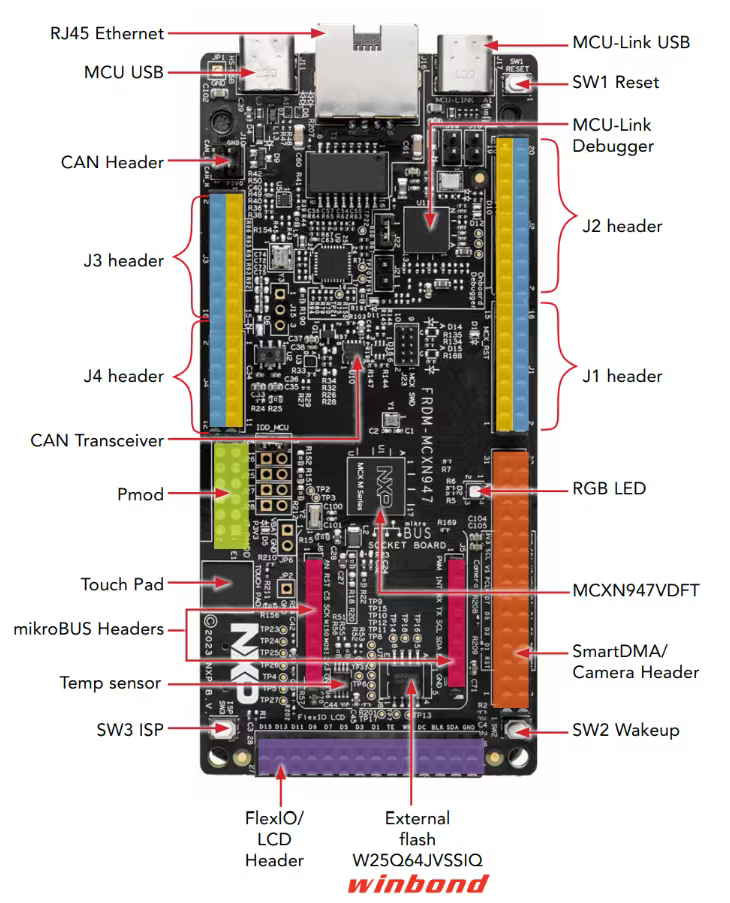
\includegraphics[width=0.65\textwidth]{obrazky-figures/frdm-mcxn947.png}
    
    \caption{Vývojová deska NXP FRDM-MCX947 \cite{nxp_FRDM_MCXN947_getting_started}}
    \label{fig:frdm-mcxn947}
\end{figure}

\subsubsection{NXP MCXN947}
Centrem mikrokontroléru MCXN947 jsou dvě jádra Arm® Cortex-M33 nové generace, pracující až na frekvenci 150 MHz. Jádro Cortex-M33 oproti předchozí generaci - Cortex-M3 je postaveno s novější instruční sadou ARMv8-M, která nabízí větší míru bezpečnosti v podobě TrustZone, jež umožňuje rozdělení paměťového prostoru na zabezpečenou (Secure World) a nezabezpečenou oblast (Non-Secure World). Dále jádro poskytuje možnost zvýšení výkonu pomocí integrovaného rozšíření DSP (Digital Signal Processor), které umožňuje efektivnější zpracování digitálních signálů a numerických výpočtů. \cite{nxp_MCX_Nx4x_Reference_Manual}

Z hlediska paměťových zdrojů nabízí MCXN947 512 KB paměti SRAM s podporou detekce a opravy chyb (Error Correction Code či zkráceně ECC). Pro zvýšení výkonu systému je čip vybaven několika typy rychlé paměti cache. Mikrokontrolér dále poskytuje 2 MB integrované flash paměti a pro programy s vyššími požadavky na úložiště je možné paměť rozšířit o dalších 8 MB prostřednictvím externí paměti typu flash připojené přes rozhraní Quad-SPI (QSPI). \cite{nxp_MCX_Nx4x_Reference_Manual}

Pro implementaci různorodých aplikací a variabilitu systému postavených na tomto čipu, MCXN947 nabízí širokou škálu periferií, které mohou být zajímavé z pohledu vývoje digitálního záznamníku. Mohou být například využity základní časovače v podobě CTIMER a CSTIMER, přes komunikační periferii LP\_FLEXCOMM, jež může být nastavena pro komunikační rozhraní I\textsuperscript{2}C, UART či SPI, nechybí ani podpora pro Ethernet a vysokorychlostní přenosy pomocí standardu USB 2.0 s Universal Serial Bus Full Speed Host and Device Controller (USBFS), který podporuje protokol OTG. Pro práci s paměťovými kartami je do čipu integrován Ultra Secured Digital Host Controller (uSDHC), který zprostředkovává komunikaci se SD, SDIO a MMC kartami. Čip MCXN947 také poskytuje tři instance A-D převodníku a taktéž tři komparátory. \cite{nxp_MCX_Nx4x_Reference_Manual}


\subsection{Raspberry PI - mikrokontrolér postaven na Linuxu}
Jednou z nejvýkonnějších možností pro implementaci digitálního záznamníku v podobě dedikovaného zařízení je využití mikroprocesorových platforem s operačním systémem Linux, přičemž nejznámějším zástupcem této kategorie je Raspberry Pi. Tato platforma spadá do kategorie jednodeskových počítačů (SBC – Single Board Computer), které kombinují výpočetní výkon a pružnost standardních počítačových systémů s rozhraními vhodnými pro práci s externími periferiemi.

Raspberry Pi je nízkonákladový minipočítač, de facto dnes už rodina počítačů, postavených na procesorech společnosti ARM, které podporují běh různých operačních systémů, nejčastěji Raspberry Pi OS. Raspberry Pi oproti klasickým mikrokontrolerům (MCU) poskytuje vyšší výpočetní výkon, taktéž i větší množství operační paměti (RAM) a podporuje také multitasking, umožňující běh více aplikací či procesů současně.

Raspberry Pi existuje v několika verzích, proto bude následný text věnován modelu Raspberry Pi Zero 2 W, který představuje rozumné parametry pro implementaci digitálního záznamníku v podobě dedikovaného zařízení. Model Zero 2 W je vybaven čtyřjádrovým procesorem Broadcom BCM2710A1 založeným na jádru ARM Cortex-A53 s taktem 1 GHz a disponuje 512 MB nízkoenergetické operační paměti SDRAM typu LPDDR2. Raspberry Pi Zero 2 W disponuje jedním USB portem typu micro-B, jenž podporuje režim OTG (On-The-Go) a umožňuje tak připojení externích zařízení, jako jsou USB flash disky či další periferie. Úložnou kapacitu zařízení lze jednoduše rozšířit díky přítomnosti slotu pro microSD kartu, která zároveň slouží jako primární úložiště operačního systému. Model Zero 2 W obsahuje také integrovaný bezdrátový komunikační modul podporující Wi-Fi standardu 802.11 b/g/n pracující v pásmu 2,4 GHz, díky kterému lze snadno implementovat digitální záznamník s podporou vzdáleného úložiště (viz. kapitola \ref{zapis_na_vzdalene_uloziste}).

\begin{figure}[h]
    \centering
    \includegraphics[width=0.85\textwidth]{obrazky-figures/raspberry_pi_zero_2w.png}
    
    \caption{Raspberry Pi Zero 2W vývody (pinout) \cite{arduino_shop_due}}
    \label{fig:raspberry-pi-zero-2w}
\end{figure}

Raspberry Pi tedy vypadá jako slibná varianta pro implementaci digitálního záznamníku, má však i své nevýhody. Hlavním omezením Raspberry Pi Zero 2 W je obecně nedostatek komunikačních periferií, platforma totiž disponuje pouze jedním modulem UART, jedním modulem SPI a jedním modulem I\textsuperscript{2}C. 
Tento omezený počet periferií může značně limitovat další rozšiřování zařízení o senzory či externí moduly. Například komplikace může nastat pouze při řešení vkládání časových razítek do záznamů, deska bohužel neobsahuje interní obvod reálného času, nabízí se  tedy využít jako referenční zdroj času, časovač (Timer) se softwarovým přerušením, druhou variantou je připojení záznamníku k síti a získat čas pomocí NTP (Network Time Protocol). Alternativním řešením se nabízí dokoupit externí obvod reálného času, to by znamenalo, že už by nebylo možné rozšířit zařízení o další periferie komunikující pomocí rozhraní I\textsuperscript{2}C, jelikož RTC moduly toto rozhraní většinou využívají, tedy sníží se možnost budoucích rozšíření.

\subsection{Shrnutí výběru platformy}
Jaká je tedy nejvhodnější platforma pro implementaci digitálního záznamníku ve formě dedikovaného zařízení? Vybral jsem FRDM-MCXN947 od společnosti NXP Semiconductors, jelikož poskytuje největší kompromis a nabízí nejvíce možností, z jakých komponent výsledný záznamník složit.

Alternativa Arduino Due, za svoji cenu za mě dostatečný poměr cena/výkon, jak je vidno v tabulce \ref{tab:board-comparison}. Maximální taktovací frekvence jádra je pouze 84 MHz, navíc to je postaveno na starší architektuře Cortex-M3. Kapacita flash paměti je oproti svým konkurentům za nižší cenu pouze 512 KB. V základu deska také neposkytuje možnost prostého rozšíření o externí uložiště jako je třeba micro SD karta, na které by mohly být získané záznamy uloženy. Také výběr, z jakého je možné vybrat řešení pro detekci ztráty napájení, je omezen.

Raspberry Pi Zero 2W naopak nabízí z vybraných možností velice dobrý poměr cena/výkon, obsahuje vysoce výkonný čip BCM2711 s taktem až 1.5 GHz a nabízí prostor, kde mohou být uloženy získané záznamy, a to konkrétně na micro SD kartě. Nicméně obtížněji by se řešilo vkládání časových značek a možná rozšíření v podobě doplňujících periferií.

\begin{table}[h]
    \centering
    \renewcommand{\arraystretch}{1.2}
    \begin{adjustbox}{max width=\textwidth} % Automatické přizpůsobení šířce stránky
    \begin{tabular}{|l|c|c|c|}
        \hline
        \textbf{Parametr / Platforma}   & \textbf{Arduino Due}  & \textbf{FRDM-MCXN947} & \textbf{Raspberry Pi} \\ 
        \hline
        \textbf{Typ čipu}               & ATSAM3X8E             & MCXN947               & BCM2711               \\ 
        \hline
        \textbf{Typ jádra}              & ARM Cortex-M3         & ARM Cortex-M33        & ARM Cortex-A53        \\ 
        \hline
        \textbf{Architektura jádra}     & 32-bit                & 32-bit                & 64-bit                \\ 
        \hline
        \textbf{Taktovací frekvence}    & 84 MHz                & 150 MHz               & 1.5 GHz               \\ 
        \hline
        \textbf{Operační paměť}         & 96 KB                 & 1 MB                  & Až 8 GB LPDDR4        \\ 
        \hline
        \textbf{Flash paměť}            & 512 KB                & 2 MB                  & MicroSD               \\ 
        \hline
        \textbf{Spotřeba }              & -                     & -                     & -                     \\ 
        \hline
        \textbf{Pořizovací cena}        & 2 058 kč (50,82€)                    & 593 Kč                & 459 Kč  \\ 
        \hline
    \end{tabular}
    \end{adjustbox}
    \caption{Porovnání vývojových desek Arduino Due, FRDM-MCXN947 a Raspberry Pi}
    \label{tab:board-comparison}
\end{table}
% ----------------------------------------------------
% DALSI NAZVY: Volba datového úložiště, Výběr externího uložiště pro záznam dat, Možnosti způsobu ukládání získaných dat
\section{Přístupy k ovládaní úložiště}
Obecný popis, proč je potřeba externí uložiště, že by se data mohla ukládat i v RAM paměti, ale že by tam moc dlouho nevydržela, 

\subsection{SDIO}

\subsection{SPI}

\subsection{Quad-SPI flash}


% ----------------------------------------------------
% DALSI NAZVY: Volba datového úložiště, Výběr externího uložiště pro záznam dat
\section{Možnosti správy dat - souborové systémy}
V předchozí části práce byla vybrána základní deska NXP FRDM-MCXN947 s mikrokontrolérem MCXN947, který bude sbírat data pomocí vstupní periferie, a tato data také zpracovávat pomocí jádra. Taktéž je vybráno externí úložiště, na které budou získaná data uložena, tím bude SD karta, konkrétněji SDHC karta. Data na tomto externím úložišti je třeba nějak organizovat, spravovat, aby mohla být v budoucnu nějakým způsobem interpretována a také popřípadě je třeba zajistit konzistenci a perzistenci uložených dat. K tomu účelu lze využít například souborový systém, databázový systém nebo data uchovávat v surovém (raw) formátu. Každý z těchto přístupů má svá specifika, nicméně data, která budou zaznamenávaná vyvíjeným záznamníkem, budou nestrukturovaná, rozhodl jsem se vybrat souborový systém. Souborový systém organizuje data přirozeně do souborů a složek a hodí se zejména pro již zmíněné ukládání nestrukturovaných dat. Pod pojmem nestrukturovaná data rozumíme taková data, která nejsou organizována jednotně v tabulkách (relacích) nebo databázových strukturách, ale mohou být ukládána do více typů souborů v různých formátech a umístěna do různorodých adresářových struktur. Tento přístup přináší výhodu, lze například získané záznamy hierarchicky členit, a zároveň umožňuje snadné přizpůsobení implementované logiky záznamníku pro ukládání i jiných typů dat. Díky tomu je záznamník obecněji využitelný pro různé typy záznamu. \cite{weka_structured_unstructured_data, virginia_tech_file_database_systems}

se  může proto existovat logika speciální pro danou aplikaci, jakou je třeba, anebo lze využít již vytvořené komponenty k tomu určené, mezi které patří i souborové systémy (File Systems).

Obecný popis, souborový systém je zodpovědný za organizaci, správu a přístup k datům na zvoleném úložném médiu.

\subsection{FATFS}
\label{fatfs}
Prvním z představených souborových systémů je FAT File System (FATFS), který je implementován v podobě lehké softwarové knihovny pro mikrokontroléry a vestavěné systémy implementující podporu souborového systému FAT/exFAT. FATFS se řadí mezi hierarchické souborové systémy založené na alokační tabulce souborů (File Allocation Table – FAT), ve kterých jsou data organizována do logických jednotek označovaných jako shluky (clusters). Každý soubor uložený na úložném médiu se tak skládá z jednoho nebo více těchto shluků, přičemž informace o jejich návaznosti jsou uloženy právě v alokační tabulce FAT. \cite{recoverit_fat_filesystem, elm_fat_filesystem_docs}

\begin{figure}[h]
    \centering
    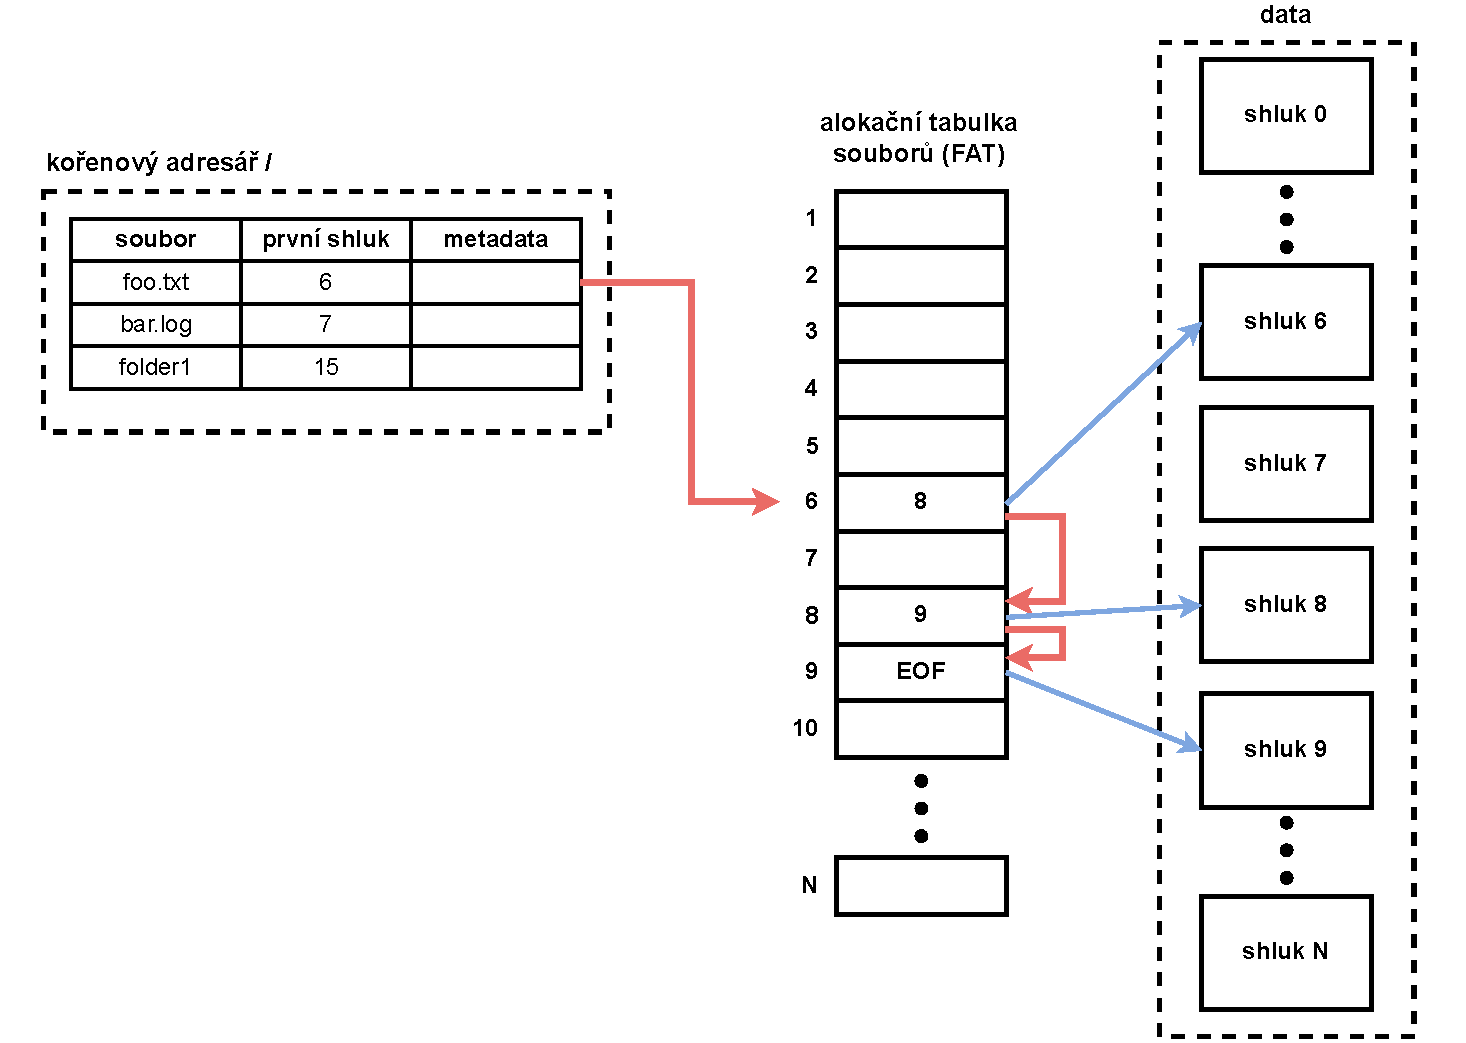
\includegraphics[width=0.80\textwidth]{obrazky-figures/fat_file_system-cz.pdf}
    
    \caption{Souborový systém s alokační tabulkou souborů \cite{recoverit_fat_filesystem}}
    \label{fig:fat-file-system-structure}
\end{figure}

Fyzické úložiště v systému FAT je rozděleno do několika oblastí, konkrétně do zaváděcího záznamu (Boot Record) ležícího v rezervované oblasti (Reserved Area), který obsahuje informace nutné pro inicializaci a načtení souborového systému, alokační tabulky FAT1 a FAT2, které spravují umístění jednotlivých shluků.  Za nimi se nachází oblast kořenového adresáře (Root Directory), ve které jsou umístěny záznamy o souborech a adresářích nejvyšší úrovně. Poslední část tvoří datová oblast (Data Area), kde jsou samotné soubory a podadresáře fyzicky uloženy.

\begin{figure}[h]
    \centering
    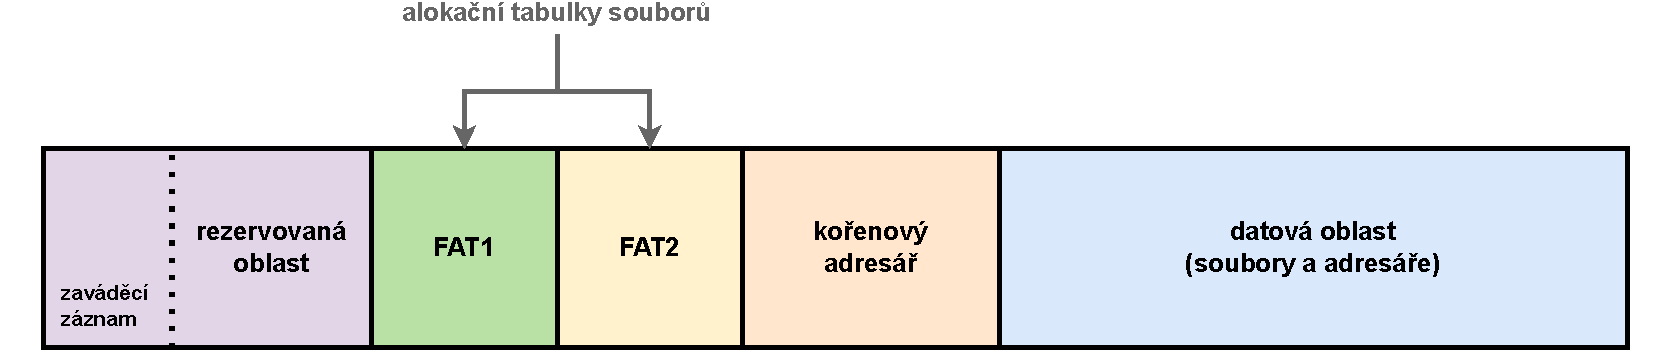
\includegraphics[width=1.00\textwidth]{obrazky-figures/fatfs_structure-cz.pdf}
    
    \caption{Oblasti souborového systému FAT \cite{recoverit_fat_filesystem}}
    \label{fig:fatfs-structure}
\end{figure}

% Jaky je rozdil mezi FAT32 a FATFS?
V dnešní době existuje několik variant systému FAT, mezi nejznámější patří FAT12, FAT16, FAT32 a exFAT. Pro úložná média typu SDHC karet se obvykle volí FAT32, neboť nižší varianty, jakou je třeba FAT16, omezují maximální kapacitu úložného média pouze na 4 GB, což je pro dnešní aplikace často nedostatečné. Z tohoto důvodu i dnešní implementace FATFS podporují 32bitovou LBA či 64bitovou LBA variantu, které podporují mnohem větší kapacitu uložišť. \cite{elm_fat_filesystem_app_note}

FATFS v současnosti představuje jeden z nejrozšířenějších souborových systémů pro použití ve vestavěných aplikacích, a to zejména díky své nízké paměťové náročnosti (nízký memory footprint) a snadné přenositelnosti mezi různými hardwarovými platformami. Významnou předností této knihovny je také široká možnost konfigurace, která umožňuje volby krátkých a dlouhých názvů souborů (Long File Name - LFN), navíc v různých formátech ANSI/OEM či Unicode. Pro velmi velká uložiště lze využít podporu exFAT s 64-bitovým adresováním bloků (LBA) a GPT (GUID Partition Table) pro práci s diskovými oddíly o velké kapacitě. FATFS také podporuje více fyzických jednotek či oddílů současně, variabilní velikost sektorů a různé kódové stránky. Knihovna rovněž obsahuje podporu pro volitelná rozhraní API, I/O buffering a režim pouze pro čtení. V případě použití v aplikaci běžící nad operačními systémy reálného času (RTOS) je výhodou této knihovny její bezpečnost, jelikož je garantována bezpečnost při práci ve vícevláknovém prostředí. \footnote{Knihovna FATFS je takzvaně Thread Safe.} \cite{elm_fat_filesystem_module}

% FAT is pretty bad on Flash devices because the low numbered sectors get rewritten frequently. Devices like USB sticks have wear levelling code, but if you're accessing raw hardware wear is a potential issue.

\subsection{LittleFS}
Alternativou k souborovému systému FATFS může být blokový (Block-Based) souborový systém LittleFS, který je podobně jako FATFS implementován ve formě odlehčené softwarové knihovny určené primárně pro vestavěné systémy a mikrokontroléry.  Tento systém byl vyvinut s ohledem na specifika flashových pamětí, aby se rovnoměrně rozdělil zápis na jednotlivé bloky a nebyly první bloky vytíženy více než ty s většími indexy.

\begin{figure}[h]
    \centering
    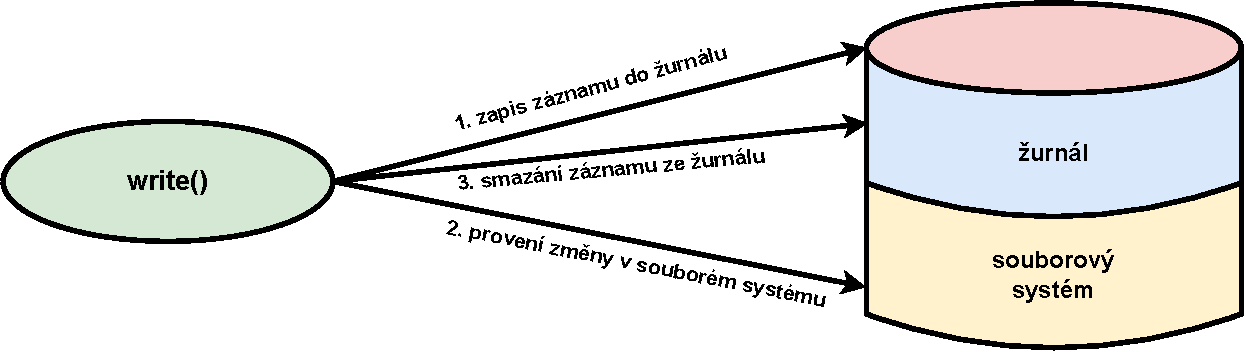
\includegraphics[width=0.95\textwidth]{obrazky-figures/journaling-cz.pdf}
    
    \caption{Průběh zápisu do souboru spravovaným žurnálovacím souborovým systémem \cite{architecture_and_design_of_the_linux_storage_stack}}
    \label{fig:journaling}
\end{figure}

% First we have the non-resilient, block based filesystems, such as FAT and ext2. These are the earliest filesystem designs and often the most simple. Here storage is divided into blocks, with each file being stored in a collection of blocks. Without modifications, these filesystems are not power-loss resilient, so updating a file is a simple as rewriting the blocks in place.
% https://github.com/littlefs-project/littlefs/blob/master/DESIGN.md

Souborový systém LittleFS využívá pokročilý mechanismus atomického zpracování známého z databázových systémů, kdy je každá operace buď kompletně dokončena, nebo v případě selhání či výpadku napájení zcela zrušena. K tomu je využit mechanismus žurnálování (journaling), který je využíván v pokročilých souborových systémech jako je ext3, XFS či ext4. Operace nad souborovým systémem jsou nejprve zaznamenány do speciální struktury (logu) před jejich fyzickým provedením. Pokud by došlo k selhání, jakým je například výpadek napájení, souborový systém se může spolehlivě vrátit do konzistentního stavu.

V souborovém systému LittleFS se k záznamu změn využívá technologie páry metadat (Metadata Pairs). Při každé operaci jsou měněna metadata souborového systému, přičemž tato metadata musí být aktualizována (měněna) atomicky. K změně jsou využity dvě speciální oblasti, označované jako metadata páry, které jsou opatřeny kontrolními součty (Checksum) a čísly revizí (Revision Count). Při každém zápisu se střídavě aktualizuje jeden ze dvou bloků metadat, přičemž druhý blok vždy uchovává předchozí konzistentní stav. Pokud by tedy došlo k selhání zápisu, souborový systém může jednoduše detekovat poškozený (Corrupted) stav a obnovit data z druhého, neporušeného bloku. \cite{nxp_the_design_of_the_little_filesystem}

Pro samotná data (Non-Meta Data) souborový systém LittleFS používá techniku Copy-on-Write (COW). Tato technika zajišťuje konzistenci dat tak, že při každém zápisu jsou aktuální (nová) data nejprve zapsána do volných bloků a teprve po úspěšném dokončení zápisu jsou bloky s neaktuálními/starými daty označeny jako volné. Pokud by tedy došlo během zápisu k chybě nebo výpadku napájení, systém se jednoduše vrátí k původním, neporušeným blokům, a tím zabrání ztrátě nebo poškození dat. \cite{nxp_the_design_of_the_little_filesystem}

Hlavními výhodami souborového systému LittleFS jsou tedy šetrnost k paměťovým médiím, nad kterými systém operuje, a také velmi nízká paměťová náročnost jak na velikost programového kódu ve flash paměti, tak na množství operační paměti RAM potřebné k jeho provozu. Dalším významným přínosem jsou již výše zmíněné pokročilé mechanismy známé z databázových systémů, zejména žurnálování a atomické operace, které umožňují zachovat souborový systém v konzistentním stavu i v případě neočekávaných selhání nebo výpadků napájení. \cite{nxp_the_design_of_the_little_filesystem}

Žurnálovací souborový systém LittleFS má ale také své nevýhody. Jednou z nejvýznamnějších je absence kompatibility při použití běžných paměťových médií, jakými jsou například SD či microSD karty, se standardními operačními systémy osobních počítačů, jakými jsou třeba Windows, Linux a MacOS. Data uložená pomocí LittleFS tak nejsou přímo čitelná na běžném počítači bez použití dodatečného softwarového nástroje (Wrapperu). \cite{cnx_software_little_fs}

\subsection{Chan FATFS}



% ----------------------------------------------------

\section{Výběr řízení přístupu k získaným datům}
\label{vyber_rizeni_pristupu_k_ziskanym_datum}
Důležitým prvkem digitálního záznamníku je také přístup k získaným datům, jak již víme, že data budou ukládána na SD kartu, respektive SDHC kartu a budou organizována a spravována souborovým systémem FatFs. Nutné je také připomenout, že jedním z požadavků na realizaci zařízení v této bakalářské práci je přístup k zaznamenaným datům bez nutnosti vyjmutí fyzického média. V úvahu připadávají varianty využívající USB či Ethernet, které vývojová deska NXP FRDM-MCXN947 nabízí, nicméně vzhledem k bezpečnostním restrikcím společnosti NXP není možné zařízení připojit k síti pomocí Ethernetového rozhraní. Tato skutečnost tedy omezuje dostupné možnosti přenosu dat pouze na komunikační protokoly nad rozhraním USB. 

% Mozna zde dopsat ze to uplne nezalezi na FS
% A file system defines how the files are organized in the storage media. The USB mass storage class specification does not require any particular file system to be used on conforming devices. Instead, it provides a simple interface to read and write sectors of data using the Small Computer System Interface (SCSI) transparent command set. As such, operating systems may treat the USB drive like a hard drive, and can format it with any file system they like. https://docs.silabs.com/protocol-usb/1.3.0/protocol-usb-msc-scsi/

\subsection{USB Mass Storage}
\label{usb_mass_storage}
První z možností pro zajištění přístupu k datům uloženým na SD kartě, respektive SDHC kartě, představuje použití standardu USB Mass Storage (MSC), vypracovaného v roce 1998 organizací USB-IF (USB Implementers Forum). Tento standard umožňuje, aby zařízení vystupovalo vůči hostitelskému systému jako standardní blokové zařízení (Block Device), host má tedy přímý přístup k celému uložišti. Protokol je dnes stále využíván a také podporován majoritní většinou moderních operačních systémů jako Microsoft Windows, operační systémy založené na Linuxu, tedy Ubuntu, Mint, Debian, ale také i Mac OS. Vyčíst data z SD karty či zapsat data na SD kartu lze tedy zvládnout téměř z kterékoliho osobního počítače.

Tento protokol rozlišuje dva komunikační prvky, prvním z nich je Mass Storage host, tedy zařízení, které aktivně řídí přístup k úložišti a provádí operace čtení a zápisu dat, tím je typicky osobní počítač nebo jiný hostitelský systém. Druhým prvkem je Mass Storage zařízení (Device), které je koncovým zařízením vystupující jako externí paměťové médium, tím může být například zmíněný Flash Disk či Hard Disk.

Z hlediska přenosových protokolů definuje USB Mass Storage dvě hlavní metody komunikace: Control/Bulk/Interrupt (CBI) a Bulk-Only Transport (BOT). CBI je přenosový protokol definovaný standardem USB 1.1, který kombinuje tři typy USB přenosů - řídicí (Control), blokové (Bulk) a přerušovací (Interrupt). Přenos se dále dělí na protokol přenosu dat, který využívá přenos přerušení, a protokol, který přenos přerušení nevyužívá. V současnosti nejrozšířenější metodou přenosu v rámci USB Mass Storage je transport pomocí BOT, v tomto režimu jsou data přenášena po blocích.
Součástí USB Mass Storage bývá také USB Floppy Interface (UFI), což je sada příkazů založená na SCSI-2 a SFF-8070 sadách příkazů, navržená pro jednoduchá bloková zařízení, původně určená pro USB disketové mechaniky (Floppy Disk), ale dnes běžně používaná pro základní interakci s jakýmkoliv typem Mass Storage zařízení. UFI definuje sadu příkazů pro čtení, zápis a správu paměťového média. \cite{usb_standard_ufi}

\begin{figure}[h]
    \centering
    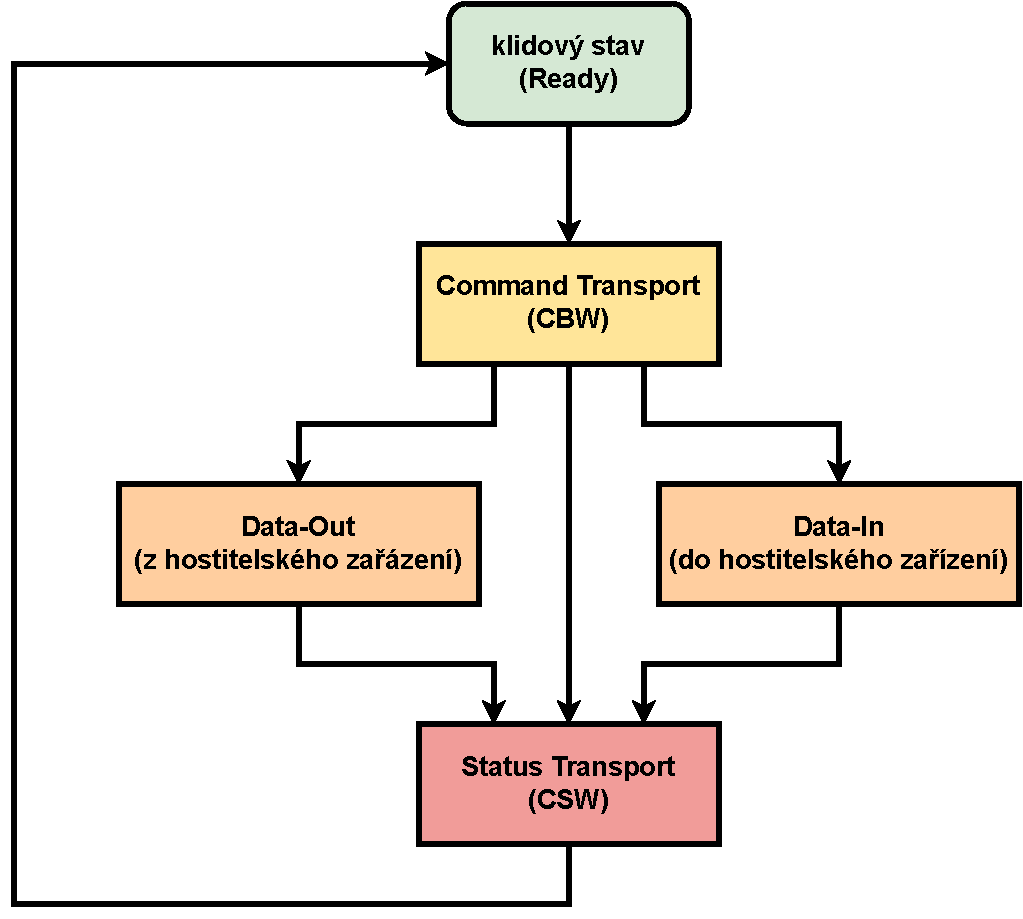
\includegraphics[width=0.65\textwidth]{obrazky-figures/mass_storage_protocol-cz.pdf}
    
    \caption{Stavový diagram USB Mass Storage protokolu \cite{silicon_labs_mass_storage_protocol}}
    \label{fig:mass-storage-protocol}
\end{figure}

Komunikace mezi hostitelem a zařízením v rámci protokolu Bulk-Only Transport (BOT) probíhá ve třech hlavních fázích, zajišťují řízený přenos příkazů, dat a zpětné vazby o provedení operace. První fází je přenos příkazu (Command Transport), během které host odešle zařízení požadavek na operaci v podobě struktury Command Block Wrapper (CBW). Tato struktura obsahuje informace o typu požadované operace (jakou je třeba inicializace, čtení, zápis), adresaci cílového sektoru na médiu a velikost přenášených dat. Pokud příkaz vyžaduje přenos dat, následuje druhá fáze - přenos dat (Data Transport). Data mohou být posílána ze zařízení do hostitele (například při čtení dat ze zařízení) nebo z hostitele do zařízení (například při zápisu na SD kartu). Přenos probíhá výhradně pomocí bulk přenosů. Poslední fází je Status Transport, v této fázi zařízení odešle zpět hostiteli strukturu CSW, která obsahuje informaci o výsledku provedené operace\footnote{v případě chyby může obsahovat další doplňující informace jako třeba množství nepřenesených dat (data residue)}. Ne všechny příkazy však vyžadují přenos dat (například příkazy pro kontrolu stavu zařízení), v těchto případech je fáze Data Transport vynechána a zařízení odesílá CSW ihned po přijetí CBW. \cite{silicon_labs_mass_storage_protocol}

% (Bulk-In/Bulk-Out). Poslední fází je Status Transport, v této fázi zařízení odešle zpět hostiteli strukturu CSW, která obsahuje informaci o výsledku provedené operace (úspěšné dokončení, chyba, množství nepřenesených dat – tzv. data residue)


\subsection{Media Transfer Protocol}
Media Transfer Protokol neboli zkráceně MTP je druhým významným protokolem umožňujícím přenos multimediálních dat mezi hostitelem a cílovým zařízením pomocí USB. MTP protokol byl navržen firmou Microsoft na základě protokolu Picture Transfer Protocol (PTP), se kterým je dodnes zpětně kompatibilní. MTP je od roku 2008 součástí USB standardu a od roku 2011 se stal standardem pro transfer souborů u zařízení využívajících operační systém Android. 

\begin{figure}[h]
    \centering
    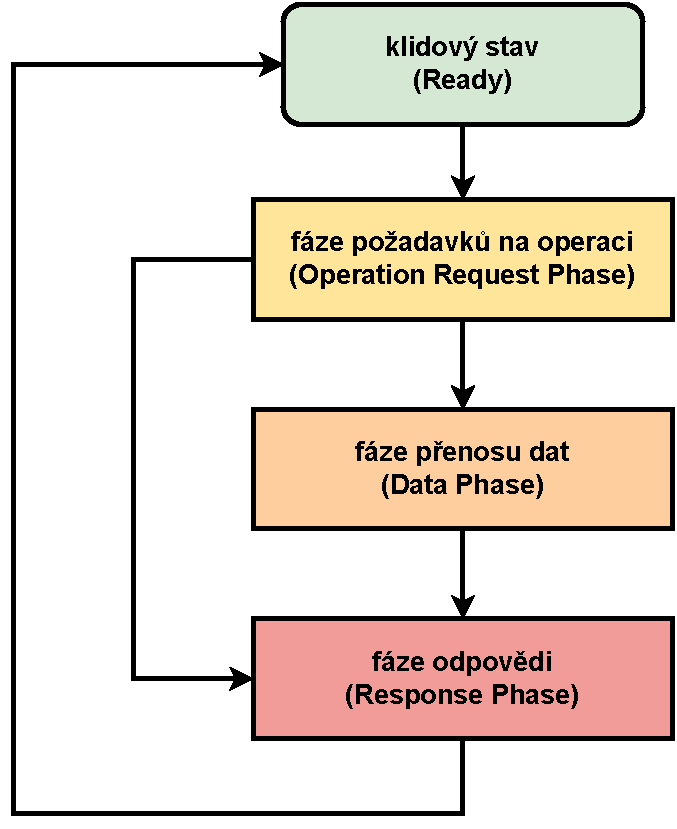
\includegraphics[width=0.50\textwidth]{obrazky-figures/mtp_phases-cz.pdf}
    
    \caption{Stavový diagram Media Transfer Protocol \cite{silicon_labs_mass_storage_protocol}}
    \label{fig:mtp-protocol}
\end{figure}

Komunikace probíhá ve formě transakcí, přičemž role komunikujících zařízení jsou iniciátor (Initiator) a odpovídající (Responder), zároveň je možné, aby si zařízení role mohly vyměnit. Transakce probíhají vždy ve třech fázích definovaných standardem, tou první je fáze požadavku na operaci (Operation Request Phase), kdy iniciátor vyšle požadavek na provedení určité operace. Následuje volitelná druhá fáze přenosu dat (Data Phase), ve které proběhne přenos dat, pokud to daná operace vyžaduje. Poslední je fáze odpovědi, ve které odpovídající odešle iniciátoru odpověď, ve které informuje o výsledku operace. Probíhající komunikace je vždy jednosměrná (Unidirectional), tedy v rámci jedné operace mohou data být pouze přenášena od iniciátora k odpovídajícímu či naopak, nikoliv však oběma směry současně. 


MTP na rozdíl od USB Mass Storage, kde je médium připojeno přímo jako blokové zařízení a hostitel má přímý přístup k souborovému systému, zde u MTP k tomu nedochází. Iniciátor tedy není zodpovědný za přímé operace se souborovým systémem, ale pouze zasílá žádosti o přenos nebo manipulaci se soubory. To znamená, že data zde nejsou interpretována připojeným zařízením (iniciátorem), ale interpretaci má na starosti odpovídající zařízení, a připojenému iniciátoru předává jen celé soubory. To přináší výhodu, že obě zařízení mohou přistupovat k datům současně (najednou). Naopak to, ale vytváří nové problémy - přes počítač nelze opravit poškozené soubory uložené na zařízení, v případě úpravy souboru je třeba nejprve soubor stáhnout do počítače, zde upravit a následně přenést zpět do zařízení.

\subsection{Human Interface Device}
Další možností pro zajištění přístupu k datům uloženým na SD kartě je využití standardu USB Human Interface Device (HID). Tento standard byl navržen původně společností Microsoft a posléze přijat jako součást USB specifikace za účelem unifikace komunikace s periferiemi, jako je klávesnice či počítačová myš. HID na rozdíl od USB Mass Storage (MSC) a Media Transfer Protocol (MTP), neslouží primárně pro práci se soubory nebo blokovými zařízeními, ale slouží jako univerzální protokol pro výměnu malých datových paketů (tzv. HID reportů). \cite{usb_standard_hid, silicon_labs_human_interface_device}

\begin{figure}[h]
    \centering
    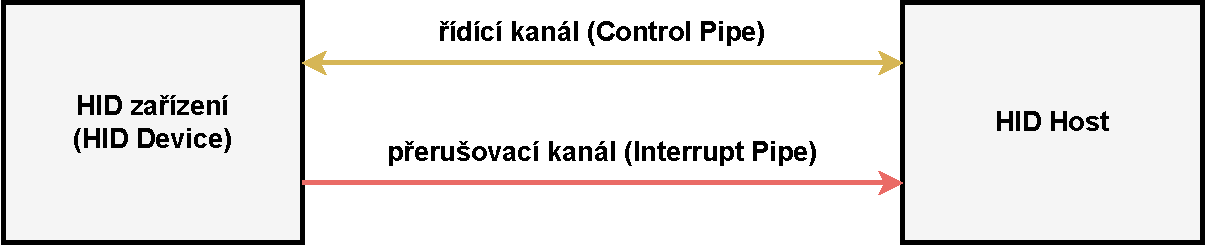
\includegraphics[width=1.00\textwidth]{obrazky-figures/hid_communication-cz.pdf}
    
    \caption{HID komunikace \cite{usb_standard_hid}}
    \label{fig:hid-communication}
\end{figure}

HID protokol definuje dvě základní role, prvním z nich je hostitelské zařízení (HID Host) a druhým je koncové zařízení (HID Device). Komunikace mezi těmito zařízeními probíhá primárně pomocí dvou typů přenosových kanálů (tzv. USB Pipe), které jsou pevně definovány standardem HID. Řídicí kanál (Control Pipe) slouží především pro inicializaci zařízení a konfiguraci přenosu dat. Přes tento kanál se přenáší tzv. HID Report Descriptor, což je struktura, která popisuje formát a význam jednotlivých HID reportů, které bude zařízení posílat hostitelskému zařízení. Řídicí kanál je taktéž využíván pro přístup ke zprávám o funkcích (Feature Reports), sloužící například k nastavování parametrů zařízení. Druhým z kanálů je přerušovací kanál (Interrupt Pipe), který slouží jako hlavní komunikační kanál pro pravidelný přenos datových rámců (reportů) mezi hostem a zařízením. Tento kanál je optimalizovaný pro malé datové pakety s nízkou latencí, typicky pro odesílání stavových informací, aktuálních měřených dat či událostí, jakým je třeba stisk tlačítka. Přerušovací přenosy probíhají periodicky, přičemž jejich frekvence je definována při enumeraci zařízení. \cite{usb_standard_hid, silicon_labs_human_interface_device}

% ----------------------------------------------------
\section{Výběr zdroje času}
\label{zdroje_casu}
Požadavkem na implementovaný digitální zaznamník  je také vkládání časových značek do záznamu, které budou využity pro následnou synchronizaci s druhým systémem. Způsobů, jak generovat časové značky, je mnoho, a je tedy nutné si na začátku stanovit základní požadavky, zda časové značky mohou být relativní (tedy například od času spuštění zařízení) či absolutní. Zároveň je však nutné při návrhu systému zvážit i další parametry, jakým je granularita časových značek, tedy časové rozlišení, s jakým budou události zaznamenávány, dále za zdroj času bude lokální nebo vzdálený. Tato kapitola představí některé ze způsobů, jak generovat časové značky, a dále rozebere jejich výhody a problémy, kterým konkrétní volby čelí. 

\subsection{Interní časovač}
Nejjednodušším způsobem pro generování časových značek je využít interní časovač, který je běžně dostupný na většině mikrokontrolérů. Interní časovač pracuje na základě přetečení čítače, který je taktován z hodinového signálu, jenž je generován interním oscilátorem nebo zvoleným hodinovým zdrojem mikrokontroléru. 

Schéma na následujícím obrázku \ref{fig:timer} znázorňuje základní strukturu interního časovače. Na vstupu se nachází multiplexer (Mux), pomocí kterého je třeba zvolit vhodný zdroj hodinového signálu, na základě kterého bude časovač reagovat, tedy inkrementovat. Tuto reakci můžeme dále ještě upravit pomocí děličky kmitočtu (Prescaler). Pomocí prescaleru lze snížit rychlost příchodu pulzů do čítače, a tím ovlivnit rychlost, s jakou časovač bude inkrementovat svou hodnotu. Na výstupu z prescaleru je napojen čítač (Module Counter), který s každým přijatým impulzem zvýší svou hodnotu o jedničku. Tento čítač je navíc svázán s modulo registrem (MOD), který definuje mezní hodnotu čítače. Jakmile čítač dosáhne hodnoty uložené v registru MOD, dojde k jeho přetečení (overflow), čítač se automaticky vynuluje\footnote{V nejjedošším případě je čítač vynulován, některé časovače, umožňují nastavit i jiné reakce, jakou je třeba dekrementace zpět na počáteční hodnotu.} a je vygenerován příznak přetečení (TOF - Timer Overflow Flag). Pokud je zároveň nastaven příznak TOIE (Timer Overflow Interrupt Enable), tak je do procesoru odeslán požadavek na vyvolání přerušení. V rámci obslužné rutiny tohoto přerušení je následně možné aktualizovat čítač časových značek a udržovat tak aktuální hodnotu pro následné doplnění do záznamů. 

\begin{figure}[h]
    \centering
    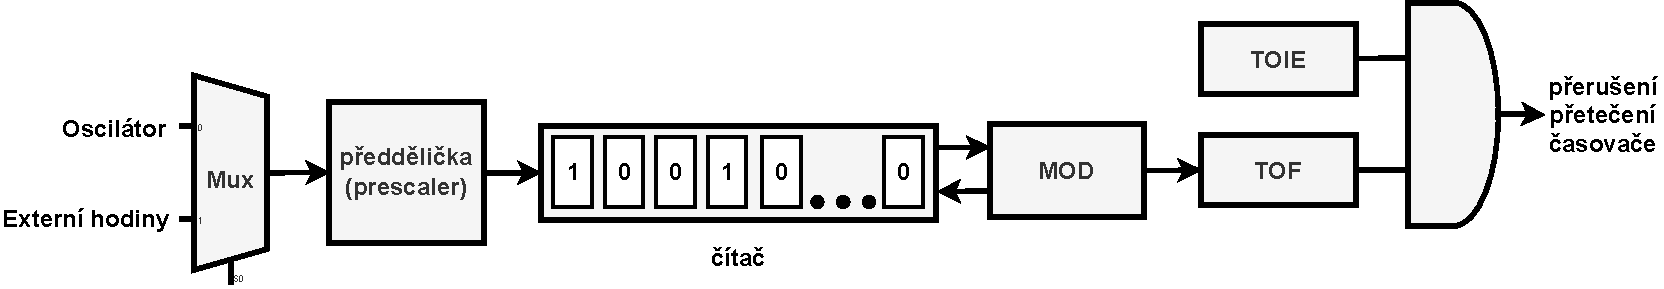
\includegraphics[width=1.00\textwidth]{obrazky-figures/timer-cz.pdf}
    
    \caption{Blokový diagram časovače}
    \label{fig:timer}
\end{figure}

Výhodou takového způsobu je výhoda v granulaci času, je možné přizpůsobit časové rozlišení. Časové rozlišení lze ovlivnit volbou hodinového zdroje, hodnotou děličky kmitočtu (prescaleru) a nastavením mezní hodnoty MOD. Lze tak snadno generovat přerušení s periodou i v řadě jednotek mikrosekund, sekundách až po výrazně delší časové úseky. V základní podobě poskytuje tento mechanismus měření relativního času, často od začátku běhu systému, pokud není použit doplňující prvek, který by umožňoval uchování či zjištění aktuálního času, jako je doplňující obvod reálného času nebo GPS modul. Právě skutečnost, že se jedná o relativní čas, přináší i určité výhody, odpadá totiž nutnost řešit komplexní problémy spojené s absolutním časem, jako jsou přechody mezi letním a zimním časem, nebo postupná odchylka interního časového základu od reálného času, která je přirozeným důsledkem výrobní tolerance oscilátorů a dalších časovacích prvků.

Takovýto způsob zproje času je sám o sobě pro záznam relativního času, často od začátku běhu systému, pokud není použit doplňující prvek, který by umožňoval uchování či zjištění aktuálního času, jako je doplňující obvod reálného času nebo GPS modul. Tím, že nepracuje s absolutním časem tj. skutečným časem, přináší další výhodu, a tou je, že není třeba řešit pokročilé problémy, které vznikají při práci s aktuálním časem, jako je nutnost řešit změny času z letního na zimní nebo třeba postupným rozjížděním času, se kterým zařízení pracuje od reálného času, jelikož časové prvky mají odchylku, jejíž význam bude časem narůstat.

Naopak mezi nevýhody použití interního časovače patří skutečnost, že takto získaný čas je pouze relativní, což v některých aplikacích nemusí být dostačující. Další nevýhodou je, že zpracování přerušení generovaných časovačem probíhá přímo v jádře systému, a tím odebírá výpočetní kapacitu, která by jinak mohla být věnována jiným úlohám. Platí přitom, že čím jemnější časové rozlišení je požadováno, tím vyšší je frekvence generovaných přerušení a tím větší je dopad na výpočetní výkon mikrokontroléru.

\subsection{Obvod reálného času}
\label{real_time_circuit}
Možné je také využít obvod reálného času (RTC - Real-Time Circuit), který je součástí většiny moderních mikrokontrolérů nebo dostupný jako samostatný externí integrovaný obvod. RTC je specializovaný časový modul navržený pro dlouhodobé uchování reálného času, tedy hodin, minut, sekund, ale často i datumu a dalších kalendářních informací.

Obvod reálného času je typicky taktován externím či integrovaným krystalem\footnote{Na obrázku \ref{fig:real-time-circuit} je krystal připojen pomocí vývodu X1 a X2 k RTC modulu.}, obvykle s rezonanční frekvencí 32,768 Hz. Tato hodnota není zvolena náhodně – odpovídá hodnotě $2^{15}$, tedy násobku dvou a umožňuje tak pomocí jednoduché děličky frekvence vydělit frekvenci na 1 Hz. Jeden kmit tak představuje jednu sekundu. Mnohé obvody reálného času také poskytují možnost připojení záložní baterie\footnote{Na obrázku \ref{fig:real-time-circuit} je baterie připojena pomocí vývodu VBAT a GND k RTC modulu.}, která slouží k udržení chodu interního časového obvodu i v případě, kdy je hlavní napájení zařízení odpojeno. Díky tomu může RTC kontinuálně uchovávat čas i po dlouhou dobu, kdy je zařízení neaktivní a není nutné čas nastavovat po každém startu zařízení. Jak již bylo zmíněno, RTC bývá často v podobě samostatných integrovaných obvodů nebo bývá integrován přímo v mikrokontroléru. Pro komunikaci mikrokontroléru s RTC jako samostatným integrovaným obvodem se obvykle využívá komunikační rozhraní I\textsuperscript{2}C, popřípadě SPI. Naopak k RTC integrovanému přímo do mikrokontroléru se přistupuje přímo prostřednictvím speciálních systémových registrů. \cite{jameco_choosing_right_real_time_clock_chip_or_module, yxc_role_of_32768_freq_in_the_circuit, medium_rtc}

\newpage

\begin{figure}[h]
    \centering
    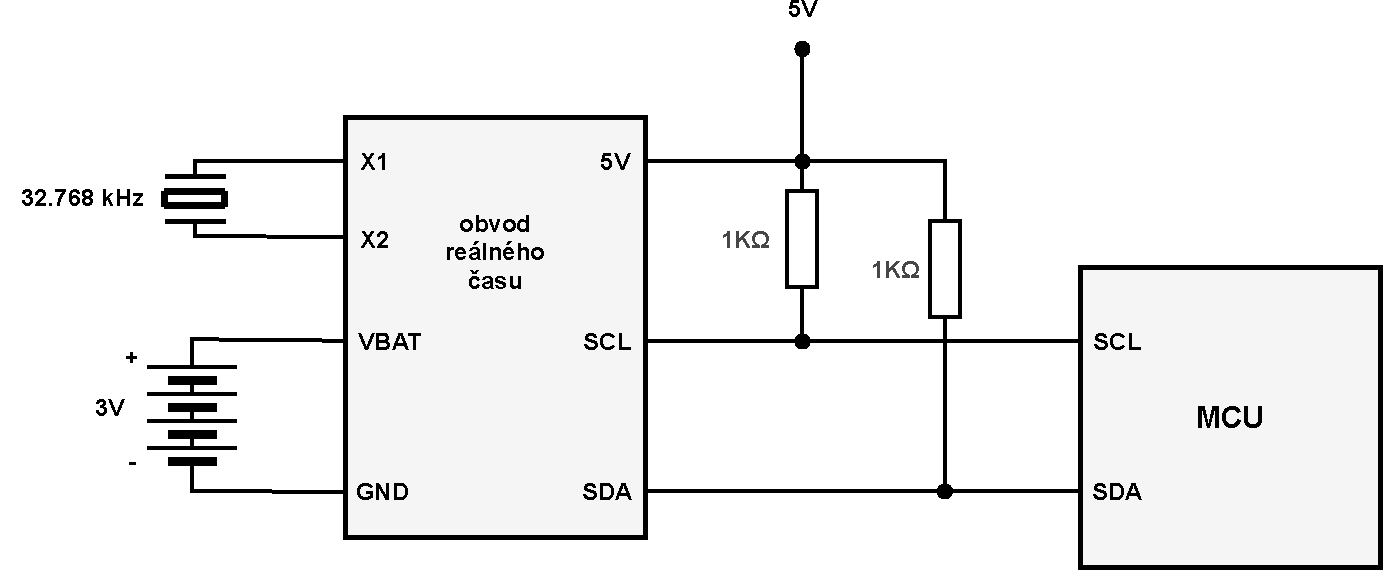
\includegraphics[width=1.00\textwidth]{obrazky-figures/real_time_circuit.pdf}
    
    \caption{Zapojení obvodu reálného času v podobě externího modulu připojeného k mikrokontroléru \cite{embed_journal_interfacing_rtc_with_microcontroler}}
    \label{fig:real-time-circuit}
\end{figure}

Obvod reálného času oproti běžnému časovači udržuje absolutní čas a dokáže jej udržovat dlouhodobě, a to i při přerušení napájení, pokud je tedy RTC vybaveno záložním napájením (například pomocí knoflíkové baterie).

Využití obvodu reálného času má, ale také své limitace či nevýhody. Zdrojem problémů může být například krystal, pomocí kterého je čas udržován, může například dojít k jeho poruše (například se krystal zastaví) či jeho rezonanční frekvence může být ovlivněna teplotními změnami. Může také nastat situace, kdy se vybije bateriový článek, poskytující napětí v době, kdy je hlavní napájení zařízení odpojeno, a je tak ztracena informace o aktuálním čase. Jedním z omezení je také minimální časové rozlišení, které je typicky nastaveno na sekundy. Mnoho standardních RTC modulů tak neumožňuje měřit a zaznamenávat čas s vyšší přesností, například v řádu milisekund či setin sekundy, což může být problémem u aplikací vyžadujících jemnější časovou osu. Také operování s absolutním časem vznikají specifické situace, jako například přechod mezi letním a zimním časem, změny časových pásem, navíc čas měřený obvodem reálného času se bude odchylovat od reálného času s narůstající dobou svého běhu, přičemž tato nepřesnost je dána konkrétním obvodem reálného času. \cite{jameco_choosing_right_real_time_clock_chip_or_module, embed_journal_interfacing_rtc_with_microcontroler, medium_rtc}

\subsection{Vzdálené zdroje času}
Další možností, jak získat časové značky, je využití vzdálených zdrojů času, které poskytují aktuální absolutní čas prostřednictvím komunikačního rozhraní. Takovými zdroji mohou být GPS satelity, NTP servery, rádiové stanice (například DCF77) a další specializované systémy. Přestože se tyto technologie mohou lišit ve způsobu přenosu a fyzikální povaze signálu (družicový, rádiový, síťový), sdílí některé principy pro určení aktuálního času. Standardně tyto systémy poskytují čas synchronizovaný vůči mezinárodnímu standardu UTC (Coordinated Universal Time) a zároveň pracují s hierarchickým modelem přesnosti označovaným jako stratum.

Koncept stratum slouží k vyjádření vzdálenosti daného časového zdroje od primárního referenčního času. Hodnotou stratum 0 jsou označeny primární zdroje času, takovými jsou například atomové hodiny. Následovné zdroje s hodnotou stratum 1 jsou přímo synchronizována se zařízeními s hodnotou stratum 0, přičemž další úrovně (stratum 2, 3 a vyšší) postupně navazují na předchozí zařízení s hodnotou stratum o jednu jednotku nižší.

\subsubsection{Globálního Polohovací Systém (GPS)}
Hodnotu stratum 0 mají například satelity globálního polohovacího systému (GPS), které právě obsahují atomové hodiny. Přesný čas satelitů je v systému GPS naprosto zásadní, neboť na jeho základě probíhá výpočet polohy přijímače. Bez znalosti velmi přesného času by totiž nebylo možné určit, za jak dlouhou dobu doputoval signál od satelitu k přijímači, a tím pádem by vznikaly chyby ve výpočtu vzdálenosti, respektive polohy.\footnote{Chyba jedné nanosekundy v tranzitním čase znaméná chybu 30cm ve zdálenosti.} GPS satelity tedy pravidelně vysílají rádiový signál (RF signál) obsahující identifikátor satelitu, hodinový signál (tj. čas) a části anmanachu obsahující například rovnici oběžné dráhy satelitu. Přijímač potřebuje tato data alespoň ze čtyř satelitů\footnote{GPS přijímač, může pro dopočitání využívá data i více než ze čtyř satelitů, aby se eliminovaly chyby vzniklé například z odchylek atovových hodin jednotlivých satelitů, či ze zanedbání faktu, že orbity satelitů nejsou zcela dokonalé kružnice.}, aby mohl dopočítat řešení čtyř rovnic o čtyřech neznámých, jehož součástí je i údaj o přesném čase pro přijímač. \cite{sparkfun_gps, time_theory_gps}

\begin{figure}[h]
    \centering
    \includegraphics[width=0.45\textwidth]{obrazky-figures/gps.png}
    
    \caption{Minimální nutná sestava čtyř GPS satelitů pro výpočet lokace a času přijímače \cite{time_theory_gps}}
    \label{fig:low-power-modes}
\end{figure}

Z pohledu přijímače má na starosti veškeré výpočty speciální GPS čipset, který integruje řadu funkcí potřebných pro správnou činnost systému. Kromě výpočtů spojených s určením polohy zpracovává i analogový rádiový signál přijatý anténou, provádí konverzi signálu do digitální podoby, spravuje řízení napájení a poskytuje rozhraní pro interakci s uživatelem. Rozdíly mezi čipovými sadami obvykle spočívají v rovnováze mezi spotřebou energie, časy akvizice a dostupností hardwaru. \cite{sparkfun_gps}

Jedna z nevýhod globálního polohovacího systému může nastat u zařízení využívaných v interiérech. Ve vnitřních prostorech může nastat problém se samotným průchodem signálu, moderní budovy často obsahují betonové stěny, kovové konstrukce, skla s metalizovanými vrstvami nebo střechy pokryté solárními panely, které představují překážky pro rádiový signál, a tak může být signál výrazně zeslaben nebo zcela pohlcen.

\subsubsection{Network Time Protocol (NTP)}
Další široce používanou technologií pro získání přesného času je síťový protokol NTP (Network Time Protocol). Tento protokol slouží k synchronizaci systémového času počítačových zařízení s časovými servery prostřednictvím sítí TCP/IP. NTP servery jsou organizovány do hierarchického systému vrstev (stratum), přičemž servery s nejnižším číslem (např. stratum 1) jsou přímo napojeny na referenční časové zdroje, jako jsou atomové hodiny nebo GPS přijímače (stratum 0). Servery na vyšších úrovních (např. stratum 2 a vyšší) získávají čas z těchto primárních zdrojů a zpřístupňují ho dále v síti.

Princip spočívá ve výměně časových značek mezi klientem a serverem. Klient odešle dotaz na NTP server ve chvíli $T_1$ a server tento dotaz přijme v čase $T_2$. Po zpracování server odešle odpověď v čase $T_3$, kterou klient přijme v čase $T_4$. Na základě těchto čtyř časových údajů lze vypočítat celkové síťové zpoždění $\delta$ a časový rozdíl (offset) $\theta$ mezi hodinami klienta a serveru. Zpoždění $\delta$ se určí jako:

\begin{equation}
    \delta = (T_4 - T_1) - (T_3 - T_2)
    \label{eq:ntp_delay}
\end{equation}
    

Zatímco rozdíl mezi klientským a serverovým časem čili offset ($\theta$), lze vypočítat dle vztahu:

\begin{equation}
    \theta = \frac{(T_2 - T_1) + (T_3 - T_4)}{2}
    \label{eq:ntp_offset}
\end{equation}

Získané hodnoty spoždění a rozdílu pak klientovi umožňují upravit systémový čas tak, aby co nejpřesněji odpovídal referenčnímu času. Protokol NTP navíc provádí více opakovaných měření a volí ty s nejnižším zpožděním, čímž zvyšuje stabilitu synchronizace i při kolísajícím síťovém připojení. \cite{sookocheff_ntp}

\begin{figure}[h]
    \centering
    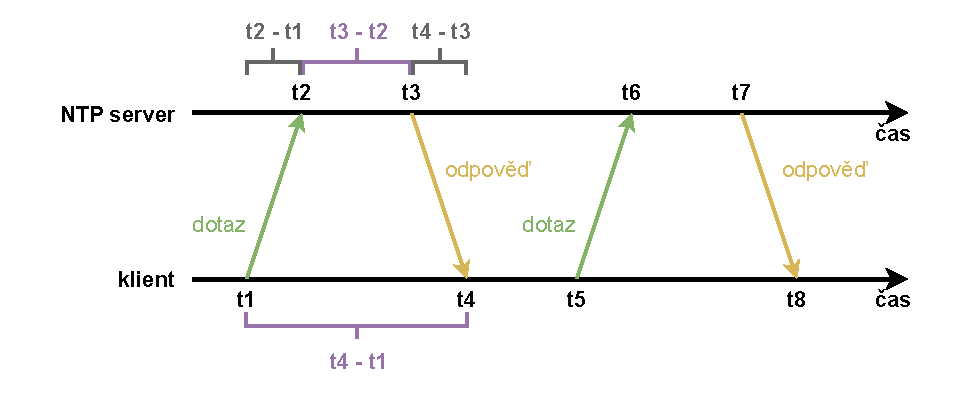
\includegraphics[width=0.95\textwidth]{obrazky-figures/network_time_protocol.pdf}
    
    \caption{Komunikace pomocí Network Time Protocol \cite{sookocheff_ntp}}
    \label{fig:network-time-protocol}
\end{figure}

NTP poskytuje přesný čas, nicméně také není vhodný pro každé vestavné zařízení vyžadující absolutní čas. Pro jeho fungování je nutná přítomnost TCP/IP zásobníku a zároveň aktivní síťové připojení k dostupnému NTP serveru. V prostředí, kde není možné garantovat trvalou konektivitu (například v mobilních, autonomních nebo izolovaných systémech), může být použití NTP omezené nebo zcela nevhodné. V takových případech je výhodnější spolehnout se na jiné zdroje času, jako je například GPS modul, nebo využít NTP pouze pro počáteční jednorázovou synchronizaci času při startu systému, kdy je připojení k síti dostupné.

% ----------------------------------------------------
\section{Výber přístupu řízení běhu aplikace}
Důležitou součástí, která bude určovat způsob, jakým bude výsledná aplikace implementována, je výběr způsobu řízení běhu aplikace. U aplikací vestavných zařízení se zpravidla rozhoduje mezi dvěma směry. Prvním z nich je implementace na holém železe, obvykle se pro tento způsob využívá anglický název bare-metal a druhou možností může být stavět program nad operačním systémem reálného času (Real-Time Operating System, zkráceně RTOS). Volba přístupu ovlivňuje výslednou architekturu. V následujících podkapitolách budou oba přístupy rozebrány, včetně jejich výhod a nevýhod. 


\subsection{Bare-Metal}
Bare-metal přístup znamená přímé řízení programu bez operačního systému, typicky s hlavní smyčkou (tzv. \emph{superloop}). Celý systém je dedikován pouze jedné aplikaci, která tak získává přímou kontrolu nad hardwarem. Program tedy přímo přistupuje k hardwarovým registrům mikrokontrolérů. 

Program se obvykle skládá ze dvou hlavních fází. První fází je inicializace, během které se nastavují systémové zdroje, konfiguruje se taktování, inicializují se periferie a případně se nastavují přerušení, nutné je podotknout, že tato fáze je provedena pouze jednou. Po dokončení inicializace přechází aplikace do hlavní smyčky, kde v nekonečném cyklu vykonává logiku programu, například zpracovává příchozí události a obsluhuje periferie. Řízení programu standardně probíhá sekvenčně, nicméně od tohoto sekvenčního provádění se odchýlí pouze tehdy, když dojde k události přerušení.

\begin{figure}[h]
    \centering
    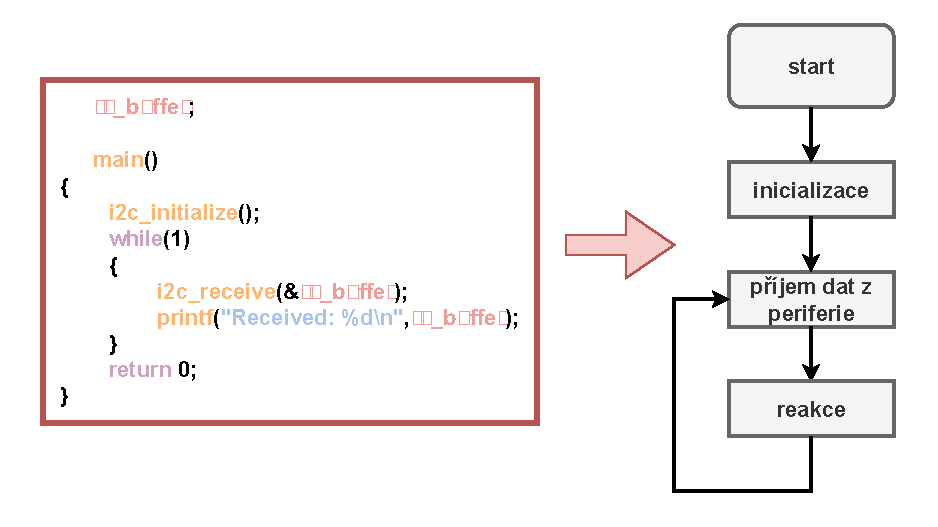
\includegraphics[width=1.00\textwidth]{obrazky-figures/bare_metal.pdf}
    
    \caption{Příklad vestavěnné aplikace využívající bare-metal přistup}
    \label{fig:bare-metal}
\end{figure}

% The bare-metal programming paradigm allows for maximum control and optimisation because the software is customised to the precise requirements of the ev embedded hardware. 
% https://medium.com/@ramjaju3737/concept-of-bare-metal-programming-in-embedded-systems-a8cd16422199
\newpage

Výhodou programování na bázi bare-metal je, že vestavné softwarové programy lze podrobně naplánovat pro konkrétní případ použití na co nejmenší úrovni, aniž by bylo nutné akceptovat režii navíc a možné chyby operačního systému. V optimálním případě tak vzniká řešení na míru, které spolehlivě plní úkoly a šetří zdroje. To má smysl vždy, pokud jsou úlohy, které mají být prováděny, zvládnutelné, takže lze zajistit co největší míru deterministického chování systému. \cite{sysgo_baremetal_vs_rtos}

Na druhou stranu, práce s holým systémem se vyskytují obtíže s zvládáním vysoké úrovně složitosti. Pokud se již tak nemalé projekty v průběhu implementační fáze nečekaně zvětší, například pokud přibudou nové funkce, které nebyly při předběžném plánování zohledněny, může být obtížné udržet si přehled. Tato obtíž může ještě narůst, pokud chybí hardwarová abstrakční vrstva nebo je navíc aplikace vyvíjená v assembleru a dokumentace k desce je nedostatečná, to může zkomplikovat vývoj i zkušeným programátorům. Nelze také opomenout, že manuální správa systémových prostředků, například ruční blokování prostředků pomocí semaforů, může být časově náročná a náchylná k chybám. \cite{sysgo_baremetal_vs_rtos}

% TODO: Zde to asi spis rozdelit na Baremetal vs. RTOS a pak uvest priklady jako FreeRTOS a ZephyrRTOS
\subsection{Operační systém reálného času}
Operační systém reálného času (RTOS) je typem počítačového operačního systému, který je navržen tak, aby byl malý a deterministický, tedy aby opakovaný vstup vedl ke stejnému výstupu. Tyto operační systémy se běžně používají ve vestavěných systémech, jako jsou lékařské přístroje a automobilové řídicí jednotky, které musí reagovat na vnější události v přísně omezeném čase. \cite{freertos_what_is_rtos}

RTOS podporuje multitasking, tedy schopnost spouštět více logických jednotek současně. Zmiňovanou nejmenší logickou jednotkou je obvykle vlákno (thread) nebo úloha (task)\footnote{Zde záleží na konkrétní implementaci RTOS například FreeRTOS používá úlohy, zatímco Zephyr RTOS pracuje s vlákny.}, které soutěží o čas procesoru a jsou vykonávána schedulerem. Na rozdíl od obecných operačních systémů, jako je Linux, které typicky využívají procesy (složené z jednoho či více vláken) izolované pomocí virtuální paměti, mnoho RTOS, zejména těch určených pro malé vestavné systémy, pracuje bez této vrstvy abstrakce. V takovém případě všechny úlohy sdílejí stejný fyzický adresní prostor a nejsou mezi sebou paměťově izolovány. Existují však i výkonnější RTOS, jako například Zephyr RTOS, které virtuální paměť a izolaci procesů podporují. \cite{freertos_what_is_rtos}

Plánovač je součástí jádra (kernelu), které představuje centrální komponentu RTOS a má na starosti správu běhu jednotlivých úloh (viz. obrázek \ref{fig:rtos-scheduling}) a přidělování procesorového času. Na rozdíl od jednoduchého sekvenčního provádění kódu v nekonečné smyčce mohou tyto úlohy běžet paralelně na základě priorit, časování a dalších parametrů. Kromě samotného plánování a přepínání mezi úlohami (tzv. přepínání kontextu) zajišťuje jádro také podporu pro synchronizaci a komunikaci mezi úlohami (např. semafory, fronty, mutexy), správu systémového času a obsluhu přerušení. Díky těmto funkcím umožňuje RTOS deterministické a přesně načasované vykonávání úloh.

\newpage

\begin{figure}[h]
    \centering
    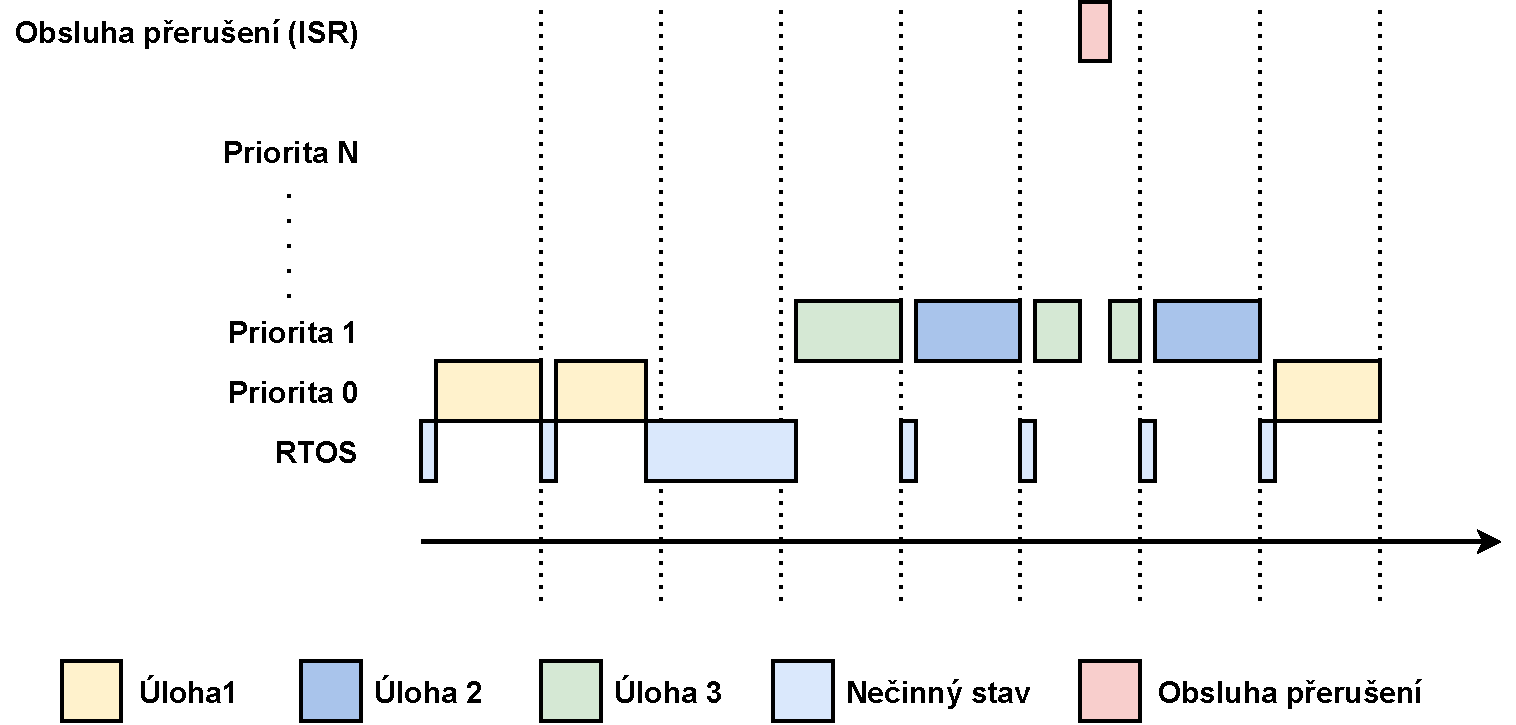
\includegraphics[width=0.90\textwidth]{obrazky-figures/rtos_scheduling.pdf}
    
    \caption{Graf znázorňující rozdělení výpočetního času, při řízení programu operačním systémem reálného času se schedulerem}
    \label{fig:rtos-scheduling}
\end{figure}

% RTOS je obvykle menší a lehčí než operační systém pro všeobecné použití, takže je vhodný pro zařízení s omezenou pamětí, výpočetní kapacitou a spotřebou energie.
Základními technickými výhodami RTOS jsou především deterministické chování, tedy schopnost reagovat na události ve striktně definovaném čase, a přesné řízení časování jednotlivých operací. To umožňuje systémům garantovat, že kritické úlohy budou vykonány ve stanovených časových limitech, bez ohledu na zátěž systému. Dále již byly nastíněny oblasti, ve kterých se operační systémy reálného času běžně uplatňují, mohou jimi být kritické systémy, jejichž selhání může mít katastrofální následky, například v robotice nebo v řídicích systémech letadel. Proto různé standardizované RTOS garantují vyšší bezpečnostní standardy a spolehlivější bezpečnostní funkce, například definované normami ISO 26262, DO-178C nebo IEC 61508.

Přestože operační systémy reálného času přinášejí řadu výhod, nelze opomenout ani jejich určitá omezení a nevýhody. Jedním z častých argumentů proti jejich použití je větší režie (overhead), která může snížit výkon a zvýšit paměťové nároky, čímž se zvyšují nároky na hardware. RTOS vnáší do systému složitost, která může ztížit jeho pochopení a ladění. Vývojáři musí být obeznámeni s rozhraním RTOS API a rozumět tomu, jak fungují úlohy, zdroje a komunikace mezi úlohami. Získání těchto znalostí může trvat delší dobu, což prodlužuje dobu vývoje a zvyšuje náklady. Použití RTOS může také zvýšit náklady na systém. Mnoho komerčních dodavatelů RTOS si účtuje licenční poplatky, které mohou být pro malé projekty nákladné.

\subsubsection{FreeRTOS}
Jednou z možností je FreeRTOS, což je open-source operační systém reálného času, který je podobný vývoji s bare-metal přístupem. FreeRTOS podporuje mnoho různých architektur a kompilátorů a je navržen tak, aby byl „malý, jednoduchý a snadno použitelný“. Jeho jádro tvoří v základu tři oblasti - správa úloh, komunikace a propojení s hardwarem. Správa úloh se stará o vytváření úloh, jak statických, tak dynamických, tak i jejich plánování a správu životního cyklu. Dále FreeRTOS poskytuje oblast zaměřenou na komunikaci mezi jednotlivými úlohami, k tomu slouží fronty (Queue). Úlohy a přerušení používají fronty k vzájemnému odesílání dat a k signalizaci použití kritických prostředků pomocí semaforů a mutexů. Poslední oblast slouží jako mezistupeň mezi hardwarově nezávislým jádrem FreeRTOS a hardwarově závislým kódem. \cite{the_architecture_of_open_source_applications}

Mezi hlavní výhody FreeRTOS patří jeho nízké nároky na systémové prostředky, což jej činí vhodným pro mikrokontroléry s omezenou pamětí a výpočetním výkonem. FreeRTOS poskytuje základní mechanismy pro plánování úloh, a to včetně prioritního plánovače s preempcí, který umožňuje přerušení aktuálně běžící úlohy ve prospěch jiné úlohy s vyšší prioritou. Velkou výhodou FreeRTOS je také jeho historie trvající přes 20 let, k dispozici je rozsáhlá dokumentace, příklady použití, mnoho výrobců, jako například NXP Semiconductors, poskytuje profesionální podporu. Z hlediska bezpečnosti FreeRTOS dodržuje přísný standard psaní kódu v souladu s normou MISRA-C, prochází statickou analýzou pomocí nástroje Coverity. Vybrané knihovny FreeRTOS byly navíc formálně ověřeny z hlediska paměťové bezpečnosti pomocí nástroje CBMC (C Bounded Model Checker). Bezpečnost systému byla rovněž potvrzena prostřednictvím certifikací SESIP™ Level 2 a PSA Certified Level 1, které vycházejí z rámce Common Criteria a hodnotí zabezpečení IoT platforem z hlediska architektury, implementace a odolnosti vůči útokům. \cite{freertos_security}

Přestože je FreeRTOS široce používán a oblíbený díky své jednoduchosti a nízké režii, nelze opomenout jeho omezení ve srovnání s robustnějšími RTOS, jakým je například Zephyr (viz. \ref{zephyr_rtos}). Nevýhodou může být omezená podpora knihoven a celkově nižší flexibilita. Není jednoduché jen tak přidat podporu na nový mikrokontrolér, jelikož portování je do značné míry jedinečné a velmi závislé na použitém procesoru a nástrojích. \cite{freertos_portability, freertos_vs_zephyr}

% Naproti tomu Zephyr RTOS má modulární, konfigurovatelný design a nabízí bohatou sadu subsystémů a knihoven. Má širokou hardwarovou podporu s více než 450 podporovanými deskami. 
% Konkrétní výhody a nevýhody FreeRTOS

\subsubsection{ZephyrRTOS}
\label{zephyr_rtos}
Zephyr RTOS je moderní open-source operační systém reálného času, který vznikl pod záštitou Linux Foundation a je aktivně vyvíjen komunitou i komerčními partnery. Zephyr je navržen jako modulární, bezpečný a škálovatelný systém, který lze přizpůsobit potřebám cílového zařízení pomocí nástroje Kconfig a popisu hardwaru ve formátu Devicetree. Typická aplikace postavená na operačním systému Zephyr je tvořena Zephyr jádrem, Zephyr moduly, vlastními moduly a aplikací, jak je možné vidět na obrázku \ref{fig:zephyr}. Zephyr moduly jsou poskytovány v rámci ekosystému operačního systému, zde patří například abstrakční vrstvy hardwaru poskytované různými výrobci čipů, jako je NXP Semiconductors, někdy je nutné si přidat vlastní moduly, těmi mohou být vlastní moduly a nakonec vlastní aplikace s logikou. Aplikaci je nutné nakonfigurovat, a jak již bylo zmíněno, k tomu se využívají nástroje Kconfig a DeviceTree. Nástroj Kconfig se používá ke konfiguraci jádra, subsystémů a softwarových knihoven a umožňuje  definovat, které části systému mají být zapnuty, jaké funkce mají být dostupné. Pro popis hardwarové struktury se Zephyr spoléhá na Devicetree, který určuje, jaké periferie jsou k dispozici, jak jsou propojeny. Popis periferií může být dále upraven nebo rozšířen pomocí overlay souborů (např. app.overlay), které přidávají nebo přepisují specifické uzly. Ze souborů Kconfig a Devicetree jsou při kompilaci vygenerovány hlavičkové soubory, které lze využít v aplikaci pro vestavěný systém. \cite{zephyr_doc_modules, embedded_summit_configure_zephyr}

\begin{figure}[h]
    \centering
    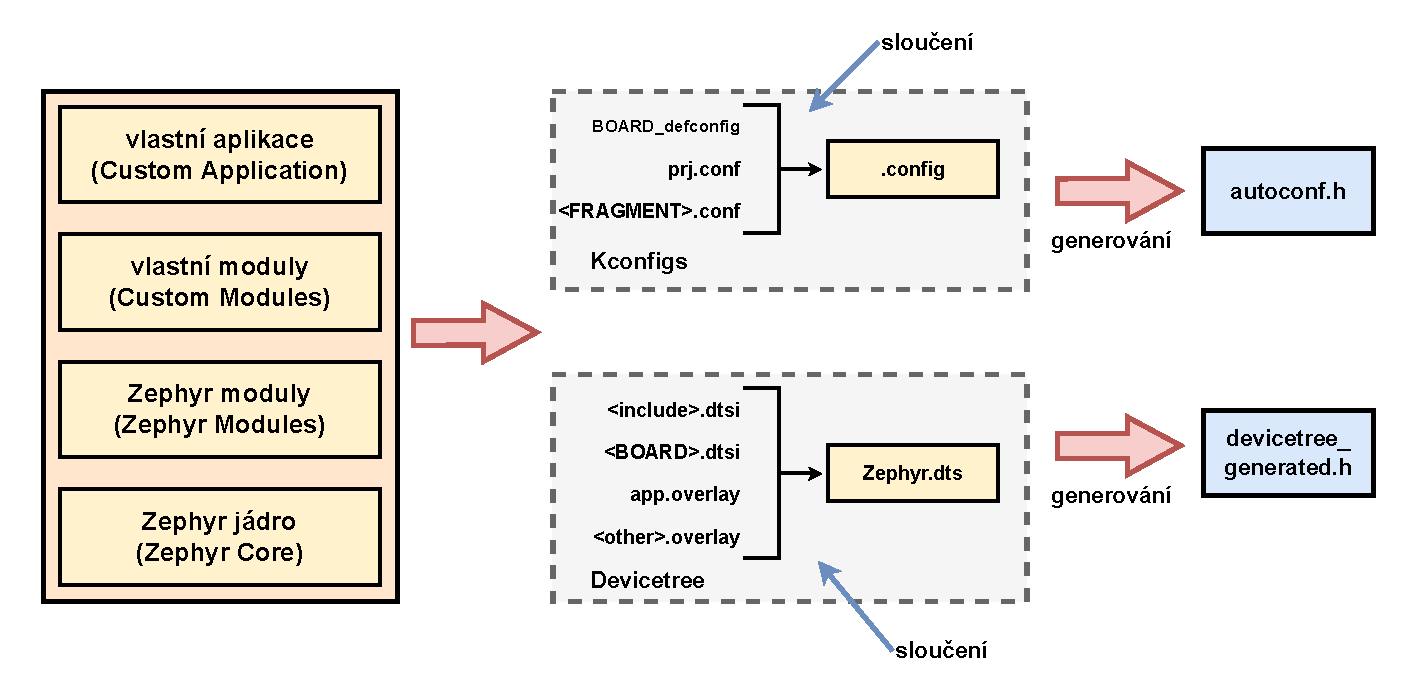
\includegraphics[width=1.00\textwidth]{obrazky-figures/zephyr.pdf}
    
    \caption{Přehled skladby projektu vyvíjeného s operačním systémem Zephyr \cite{embedded_summit_configure_zephyr}}
    \label{fig:zephyr}
\end{figure}

Mezi hlavní výhody operačního systému Zephyr patří jeho vysoká modularita a konfigurovatelnost, která umožňuje vývojářům sestavit jen ty části systému, které jejich aplikace skutečně potřebuje. Zephyr abstrahuje (mikro)jádro, HAL, middleware a komunikaci způsobem nezávislým na platformě, aplikační vrstva je tak oddělena od hardwarové vrstvy prostřednictvím abstrakcí v Devicetree a subsystémech jádra není aplikace pevně svázána s konkrétním mikrokontrolérem či deskou. Díky této abstrakci je možné aplikaci přenést na jinou desku s obdobným hardwarem zpravidla jen díky změnám v konfiguračních souborech. \cite{zephyr_advantages}

Na druhou stranu má Zephyr i své nevýhody, které mohou ovlivnit jeho vhodnost pro určité typy projektů. Vzhledem ke své komplexnosti může být učení se systému náročnější, a to zejména pro začínající vývojáře nebo pro jednodušší aplikace, kde je plně vybavený framework zbytečně robustní. I přesto, že je Zephyr dobře škálovatelný, základní velikost systému a spotřeba paměti jsou ve srovnání s minimalistickými RTOS, jako je FreeRTOS, vyšší. Další nevýhodou je, že vývojové prostředí Zephyru není na platformě Windows ještě plně dopracované. Přestože se podpora zlepšuje a základní funkcionalita je dostupná, není momentálně srovnatelná s prostředím na Linuxu, které je primární platformou pro vývoj aplikací s Zephyr operačním systémem. To je bohužel nevýhoda, jelikož v týmu, ve kterém pracují a který tento digitální záznamník bude využívat, je k dispozici výhradně systém Windows, což znesnadní budoucí vývoj případných rozšíření projektu. \cite{nabto_guide_zephyr_vs_freertos}


% ----------------------------------------------------
% Popis architektury na základě vybraných komponent. Popis blokového diagramu.

\section{Architektura systému digitálního záznamníku}
\label{architektura_systemu_digitalniho_zaznamniku}
V Předchozích kapitolách byly představeny vybrané komponenty, které lze využít k sestavení digitálního záznamníku v podobě dedikovaného zařízení. Z představených vývojových platforem byla jako základní deska zvolena vývojová deska FRDM-MCXN947 od společnosti NXP Semiconductors (viz. \ref{nxp_frdm_mcxn947}), která poskytuje dostatečný výkon, paměťový prostor a periferie, které lze využít k realizaci záznamníku.

Pro řízení činnosti záznamníku bude použit operační systém reálného času FreeRTOS, přičemž architektura firmwaru bude rozdělena do dvou hlavních úloh. První z úloh bude záznamová úloha, která bude zajišťovat průběžné získávání dat z UART periferie a jejich ukládání na paměťové médium. Druhou úlohou báde komunikační úloha, která bude zodpovědná za zpřístupnění uložených dat prostřednictvím rozhraní USB ve standardu Mass Storage Class (MSC), čímž odpadá nutnost fyzického vyjímání paměťové karty ze zařízení. Pomocí tohoto přístupu lze dosáhnout vyšší modularity, přehlednosti a současného chodu obou činností bez vzájemného blokování.

% Předchozí kapitoly představily vybrané komponenty, které lze využít k sestavení digitálního záznamníku v podobě dedikovaného zařízení. Z představených vývojových platforem, byla jako  jako základ, zvolena vývojová deska FRDM-MCXN947 od společnosti NXP Semiconductors (viz. \ref{nxp_frdm_mcxn947}), která poskytuje dostatečný výkon, paměťový prostor a periferie, které lze využít k realizaci záznamníku. Pro řízení činnosti záznamníku bude použit operační systém reálného času FreeRTOS, který umožní oddělit jednotlivé funkční části programu do samostatných paralelně běžících úloh. Přičemž architektura softwaru bude rozdělena do dvou hlavních úloh. A to konkrétně záznamová úloha, která... a druhou úlohou bude...

Firmware bude koncipován tak, aby v každém okamžiku byla aktivní vždy pouze jedna z hlavních úloh, což minimalizuje riziko konfliktu při přístupu k paměťovému médiu. Přepínání mezi úlohami bude řízeno detekcí připojení nebo odpojení USB rozhraní. V běžném režimu bude systém pracovat v záznamovém režimu a uchovávat příchozí data. Jakmile dojde k připojení zařízení k hostitelskému počítači, záznamová úloha se zastaví a aktivuje se komunikační úloha, která zpřístupní obsah úložiště jako běžný USB disk. Po odpojení USB se firmware automaticky vrátí do režimu záznamu.

Po spuštění firmware nejprve proběhne základní inicializace klíčových komponent, které budou aktivní po celou dobu běhu aplikace. V rámci této fáze se mimo jiné naváže komunikace s externím RTC modulem prostřednictvím sběrnice I\textsuperscript{2}C, ze kterého si mikrořadič přečte aktuální čas. Zjištěný čas bude následně uložen do interního RTC modulu, jenž je součástí samotného mikrořadiče. Práce s interním obvodem reálného času zrychlí přístup k systémovému času, jelikož další komunikace již nebude probíhat přes komunikační rozhraní I2C, ale přímo prostřednictvím registrů v rámci interní periferie.

Následně po úspěšné inicializaci bude spuštěna jako výchozí a dominantní úloha, záznamová úloha, která zajistí příjem dat z externího zdroje. V rámci dané varianty digitálního záznamníku pro využití firmou NXP Semiconductors bude jako vstupní periferní rozhraní využit modul LP\_FLEXCOMM, nakonfigurovaný v režimu UART. Přijatá data budou dále zpracovávána a ukládána do paměťového úložiště s využitím postupů popsaných v kapitole~\ref{klicove_koncepty_digitalnich_zaznamniku}, přičemž bude kladen důraz na efektivní využití prostředků a minimalizaci ztráty dat i při vyšších přenosových rychlostech. Správu a organizaci dat v paměťovém médiu bude zajišťovat hierarchický souborový systém FATFS, který byl již představen v kapitole \ref{fatfs}.

Samotná zaznamenaná data budou ukládána na SDHC kartu, která byla zvolena z důvodu dostatečné kapacity (až 32GB), možnosti vytvoření standardního souborového systému a snadné zpětné dostupnosti dat prostřednictvím USB Mass Storage rozhraní. K ukládání bude využit přístup s přímým zápisem, jelikož kdyby by byl využít přístup s FeRAM mezipamětí, digitální záznamník by musel nejprve přijatá data zpracovat v RAM paměti, tj. doplnit časové značky. Tato zpracovaná data by pak byla přesunuta z RAM do FeRAM, kde by byla dočasně uchována, a následně opět načtena zpět do RAM, aby mohla být zapsána do souboru na SD kartu. Ve výsledku by tedy i tento přístup vyžadoval alokaci paměťového prostoru v RAM, a tím by se výhoda použití FeRAM jako mezivrstvy ztratila. Přístup se vzdáleným uložištěm naopak nebyl zvolen, z důvodu toho, že vývojový tým společnosti NXP Semiconductors, zaměřený na bezdrátové napájení, v současnosti nedisponuje žádnou infrastrukturou pro vzdálené ukládání dat a současně je zakázáno získaná data ukládat do externích cloudových řešení.

Jakmile bude detekováno připojení k hostitelskému počítači, systém pomocí mechanismu USB OTG (On-The-Go) ověří, že došlo ke skutečnému připojení a navázání komunikace. V reakci na tuto událost se zařízení automaticky přepne do režimu Mass Storage, ve kterém bude vnitřní paměťové úložiště zpřístupněno jako běžný externí disk. Data tak budou přístupná bez nutnosti manipulovat se samotným zařízením nebo vyjímat paměťovou kartu.

\begin{figure}[h]
    \centering
    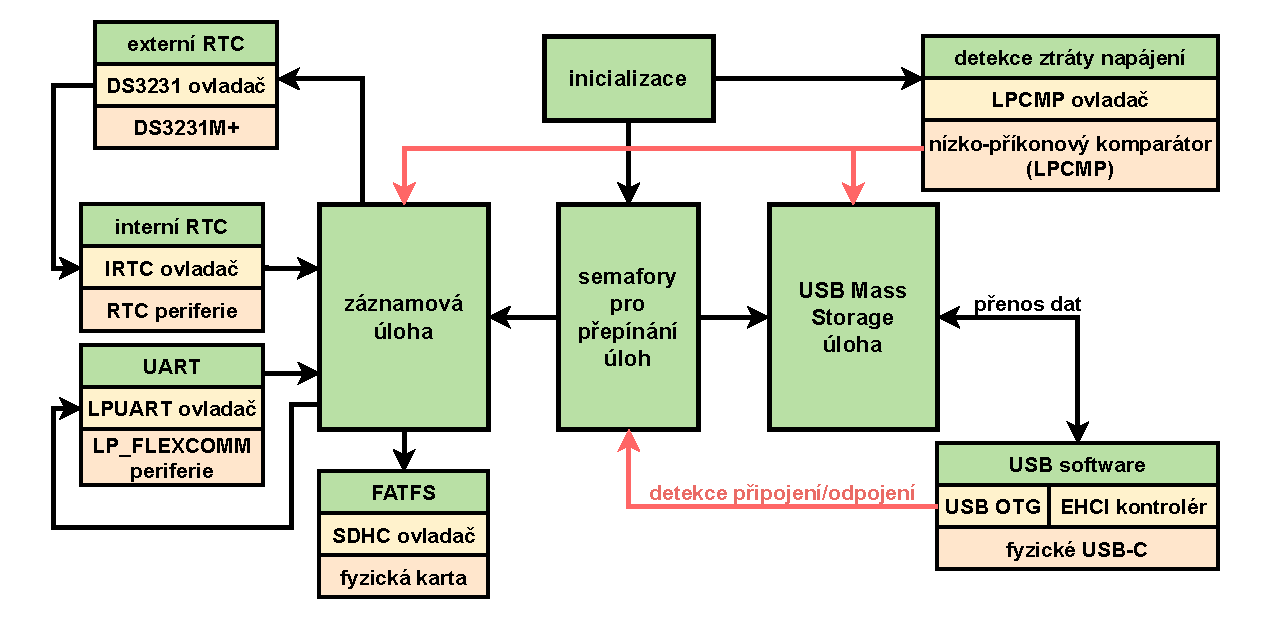
\includegraphics[width=1.00\textwidth]{obrazky-figures/system_architecture.pdf}
    
    \caption{Výsledná architektura digitálního záznamníku}
    \label{fig:system-architecture}
\end{figure}

Důležitou součástí návrhu systému je rovněž detekce ztráty napájecího napětí, která umožňuje včasnou reakci na neočekávané odpojení napájení. K tomuto účelu bude využita periferie LPCMP (Low-Power Comparator), která je součástí čipu na vývojové desce FRDM-MCXN947. Jakmile napájecí napětí poklesne pod stanovenou prahovou hodnotu, komparátor tento stav vyhodnotí a generuje událost, která informuje aplikační vrstvu o hrozícím výpadku. Od tohoto okamžiku je úkolem aplikace zajistit uložení všech rozpracovaných dat, která dosud nebyla zapsána do permanentního paměťového média, a také korektní uzavření otevřených souborů, aby bylo možné firmware bezpečně ukončit a předejít ztrátě nebo poškození dat.



% ----------------------------------------------------

\section{Volitelné rozšíření}
\subsection{Měření teploty}

% ----------------------------------------------------

\subsection{Řešení problému synchronizace času}

% ----------------------------------------------------

\chapter{Realizace hardwaru}
\label{realizace_hardwaru}

\section{Základová deska} 
V kapitole~\ref{vyber_vhodne_platformy} byl popsán proces výběru vhodné platformy pro běh firmwaru digitálního záznamníku. Jako nejvhodnější řešení se ukázalo využití vývojové desky FRDM-MCXN947 od společnosti NXP Semiconductors. Čip MCXN947 poskytuje mnoho různých periferií, které mohou být využity k realizaci digitálního záznamníku.

Samotný čip poskytuje časovače v podobě CTIMER a CSTIMER, které mohou být využity pro měření časových intervalů nebo generování periodických událostí. Dále je k dispozici flexibilní komunikační blok LP\_FLEXCOMM, který umožňuje konfiguraci až osmi nezávislých instancí komunikačních rozhraní (například I\textsuperscript{2}C, UART nebo SPI) podle aktuálních požadavků aplikace.

\section{Expanzní deska}
% Jak jsem měřil spotřebu, jak jsem spočítal hodnoty kondenzátorů 
Vybraná základová deska neobsahuje všechny potřebné komponenty k realizaci firmwaru, které byly představeny v kapitole \ref{architektura_systemu_digitalniho_zaznamniku} a pro zajištění kompletní funkcionality je nutné doplnit celý systém o expanzní desku plošných spojů, která umožní integraci všech externích komponent a rozšíří tak funkcionalitu základové desky.

\subsection{Zálohované napájení}
\label{zalohovane_napajeni_hw}
Důležitou součástí realizovaného digitálního záznamníku je zálohované napájení s detekcí ztráty napájecího napětí. Zálohované napájení lze realizovat několika způsoby, nejčastěji pomocí dobíjecí baterie (např. Li-Po nebo knoflíkového článku) nebo pomocí kondenzátoru. Nejschůdnější variantou pro danou aplikaci se ukázal být kondenzátor, respektive superkondenzátor. Na rozdíl od baterií je schopen okamžitě dodat relativně vysoký vybíjecí proud, který byl naměřen při testování spotřeby pomocí zařízení Power Profiler Kit II od společnosti Nordic Semiconductors (viz. obrázek \ref{fig:power-consumption}), při kterém se ukázalo, že vstupní proud může dosáhnout hodnot až \SI{250}{\milli\ampere}. Běžné knoflíkové články nebo malé Li-Po baterie by v tomto ohledu nemusely zajistit dostatečný proud a případně by při takové zátěži vedly k velmi krátké výdrži. \cite{nordic_semi_ppk2}

% Zaroven musi byt jmennovite napeti vyssi z duvodu
Z tohoto důvodu bylo třeba vybrat superkondenzátor, který bude vyhovovat parametrům pro využití v digitálním záznamníku. Mezi takové parametry patří zejména kapacita, která určuje, jak dlouho je zařízení schopno fungovat po ztrátě napájení. Dále bylo nutné zohlednit jmenovité napětí, které musí být vyšší než maximální napájecí napětí systému, aby nedošlo k poškození součástky.\footnote{Běžně je doporučováno volit dvojnásobek či dokonce trojnásobek napětí při kterém bude kondenzátor operovat.} Dalším důležitým faktorem je ekvivalentní sériový odpor (ESR), jenž ovlivňuje schopnost superkondenzátoru dodávat vysoký proud bez výrazného poklesu napětí, čím nižší ESR, tím lépe je tedy kondenzátor schopen poskytovat vyšší proud. Vzhledem k omezenému prostoru na expanzní desce bylo zároveň nezbytné zohlednit fyzické rozměry kondenzátoru tak, aby jej bylo možné snadno integrovat a popřípadě umožnit, aby bylo možné využít dva kondenzátory paralelně, pro zvýšení spolehlivosti systému v případě selhání jednoho z kondenzátorů. \cite{cadence_capacitor_size}

\begin{figure}[h]
    \centering
    \includegraphics[width=0.80\textwidth]{obrazky-figures/power-consumption-2.png}
    
    \caption{Výsledek měření spotřeba implementovaného záznamníku pomocí Power Profiler Kit II 
    \cite{nordic_semi_ppk2}}
    \label{fig:power-consumption}
\end{figure}

Jako vhodný kondenzátor byl tedy vybrán model SCMR14G334SRBB0 od společnosti KYOCERA AVX s kapacitou \SI{0.33}{\farad}, jmenovitým napětím \SI{7.5}{\volt} při stejnosměrném proudu a nízkým ESR, které má konkrétní hodnotu \SI{450}{\milli\ohm}. Vzhledem k relativně nízké ceně této komponenty bylo třeba jej nejprve experimentálně ověřit v provizorním zapojení (viz. schéma \ref{fig:test-capacitors}) na nepájivém poli. Kondenzátor byl v tomto testu nejprve nabíjen z laboratorního zdroje nastaveného na \SI{5}{\volt} odpovídající reálným provozním podmínkám v cílovém zařízení. Po jeho odpojení byla sledována vybíjecí křivka sledována pomocí osciloskopu.

\begin{figure}[h]
    \centering
    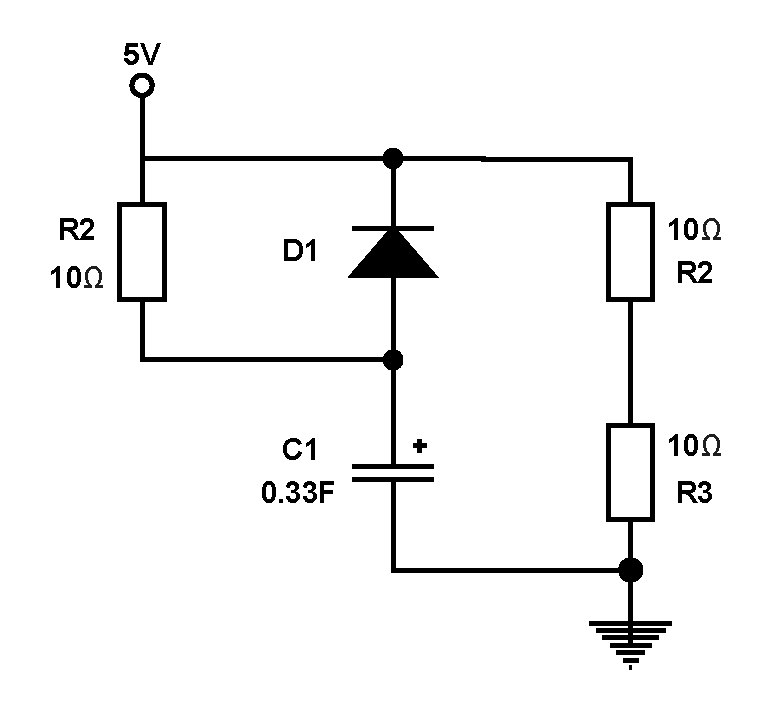
\includegraphics[width=0.440\textwidth]{obrazky-figures/test_capacitors.pdf}
    
    \caption{Obvod pro testování kondenzátoru}
    \label{fig:test-capacitors}
\end{figure}

Aby bylo možné přesně vyhodnotit, jak dlouho dokáže záznamník fungovat při napájení ze superkondenzátoru, je třeba nejprve vysvětlit několik základních skutečností souvisejících s vývojovou deskou FRDM-MCXN947, která bude napájená z výše popsaného kondenzátoru. Vstupní napětí \SI{5}{\volt} jde přes LDO (Low-Dropout Regulator), které upravuje napětí na 3V3 zásobující čip. LDO však ke své funkci vyžaduje minimální rozdíl mezi vstupním a výstupním napětím, tzv. Dropout Voltage, při kterém je tento integrovaný obvod ještě schopen pracovat. Minimální vstupní napětí potřebné pro stabilní výstup 3.3V je dáno vztahem:

\[
V_{\text{LDO Min}} = V_{\text{LDO Out}} + V_{\text{Dropout}}
\]

V případě použitého stabilizátoru, který je využit na vývojové desce FRDM-MCXN947, je hodnota Dropout Voltage rovna \SI{0.2}{\volt} a minimální napětí, kterým tedy tato deska musí být napájena, činí \SI{3.5}{\volt}. Součástí zapojení na schématu je také Schottky dioda, na které vzniká úbytek napětí, u použité součástky činí tento úbytek přibližně \SI{0.4}{\volt}. Z těchto hodnot vyplývá, že je nutné sledovat napětí vybíjejícího se kondenzátoru v intervalu od \SI{4.6}{\volt} do \SI{3.5}{\volt}, které definuje časový interval, ve kterém je provoz vývojové desky stabilní.

Následující obrázek \ref{fig:test-capacitors}, zachycuje průběh napětí z výše zmíněného testu, zaznamenaného pomocí osciloskopu, ze kterého je patrné chování napájecího napětí v čase. Z naměřených dat vyplývá, že napětí na kondenzátoru zůstává v požadovaném funkčním rozsahu od \SI{4.6}{\volt} do \SI{3.5}{\volt} po dobu přibližně 1.3 sekundy. Pokud tedy dojde ke včasné detekci ztráty napájejícího napětí, může dojít k bezpečnému ukončení programu a korektnímu uložení všech potřebných dat, která jsou dočasně uložena ve volatilní paměti RAM, což potvrzuje vhodnost zvoleného superkondenzátoru pro danou aplikaci zálohovaného napájení.

\begin{figure}[h]
    \centering
    \includegraphics[width=1.00\textwidth]{obrazky-figures/capacitor-test-osciloscope.png}
    
    \caption{Průběh napětí na kondenzátoru při vybíjení zachycený osciloskopem}
    \label{fig:test-capacitors}
\end{figure}

\newpage

Na následujícím obrázku \ref{fig:backup-power} je apk znázorněno výsledné schéma obvodu určeného k realizaci zálohovaného napájení včetně detekce ztráty hlavního napájecího napětí. Obvod zahrnuje zmíněnou Schottkyho diodu, která zabraňuje zpětnému toku proudu z kondenzátoru, a nabíjecí odpor s hodnotou $\SI{10}{\ohm}$, která byla zvolena tak, aby byl proud při nabíjení omezen na rozumnou, tedy aby zůstal pod minimální hodnotou, kterou je schopen standard USB-C, a zároveň aby nabíjení probíhalo v přiměřeném čase. Pro výpočet doby nabíjení je klíčovým parametrem časová konstanta~$\tau$, která je definována jako součin odporu~$R$ a kapacity~$C$:

\[
\tau = R \cdot C
\]

Součástí navrženého obvodu zálohovaného napájení je rovněž detekce ztráty napájecího napětí, jelikož je monitorována \SI{5}{\volt} větev vývojové desky, která překračuje maximální přípustné napětí pro přímé připojení na vstupy mikrokontroléru pracujícího s logikou \SI{3.3}{\volt}, je tedy zapotřebí využít napěťový dělič, který upravuje napěťový signál, aby mohl být zpracován periferiemi pracujícími s digitálními signály, jako jsou GPIO, nebo analogovými signály, jako je komparátor (CMP) či analogově-digitální převodník (ADC).

\begin{figure}[h]
    \centering
    \includegraphics[width=0.80\textwidth]{obrazky-figures/backup-power.png}
    
    \caption{Schéma obvodu pro detekci ztráty napájení a zálohované napájení}
    \label{fig:backup-power}
\end{figure}

\subsection{Obvod reálného času}
Pro uchovávání informací o čase a datu je využit externí obvod reálného času, konkrétně čip DS3231M+ od společnosti Analog Devices. DS3231M+ patří mezi vysoce přesné RTC čipy obsahující integrovaný oscilátor s teplotně kompenzovaným krystalem (TCXO), který zajišťuje minimální odchylku chodu v řádu několika sekund za měsíc bez nutnosti externí kalibrace. Tato odchylka specifikovaná výrobcem činí \SI{\pm2} minut za rok v teplotním rozsahu od \SI{-40}{\degreeCelsius} do \SI{+85}{\degreeCelsius}.

Obvod reálného času s čipem DS3231M+ je integrován do expanzní desky plošných spojů (viz. obrázek \ref{fig:ds3231m+}) podle vzorového zapojení, jež bylo ukázáno v datasheetu k tomuto čipu. Pro komunikaci s tímto čipem se využívá jednoduché rozhraní I\textsuperscript{2}C s využitím dvou signálových linek, kterými jsou SDA (Serial Data Line) a SCL (Serial Clock Line). Linka SDA slouží k přenosu dat mezi mikrokontrolérem a RTC obvodem, zatímco linka SCL zajišťuje synchronizaci komunikace pomocí hodinového signálu. Kromě komunikačních linek je nutné k čipu připojit napájení. Pin V\textsubscript{CC} slouží pro napájení čipu v běžném provozu, kdy je deska aktivně napájena. Pro zachování aktuální časové informace i během neaktivního stavu zařízení nebo během výpadku napájecího napětí je k dispozici pin V\textsubscript{BAT}, který je připojen ke knoflíkové baterii CR2032.

Dále čip DS3231M+ obsahuje vývod 32KHZ, který slouží jako výstup stabilního hodinového signálu o frekvenci 32 kHz. Dále je k dispozici multifunkční pin INT/SQW, který může pracovat buď jako výstup čtvercového signálu (square wave), nebo jako přerušovací výstup v případě shody časových registrů s nastaveným alarmem. Signály 32KHZ a INT/SQW nejsou v implementaci digitálního záznamníku využívány, proto jsou oba připojeny pull-up odpory k zemi. Posledním relevantním signálem je RST, který slouží k resetování RTC obvodu. V návrhu expanzní desky je vývod signálu připojen k jumperu, jehož sepnutím lze čip ručně resetovat.

\begin{figure}[h]
    \centering
    \includegraphics[width=0.80\textwidth]{obrazky-figures/ds3231m+.png}
    
    \caption{Obvod pro reálného času s čipem DS3231M+}
    \label{fig:ds3231m+}
\end{figure}

\subsection{GPS pro synchronizaci času}
Přestože integrovaný obvod reálného času DS3231M+ nabízí velmi dobrou dlouhodobou přesnost, stále jeho odchylka může činit až \SI{\pm2} minuty za rok. Mnoho aplikací vyžaduje ještě vyšší přesnost časové synchronizace, proto je expanzní deska připravena pro možnost připojení externího GPS modulu. Konkrétně se počítá s využitím modulu NEO-7M, který je schopen poskytovat přesné údaje o čase díky synchronizaci s globálním navigačním systémem.

Modul NEO-7M obsahuje integrovaný přijímač, pasivní keramickou anténu a anténní zesilovač. Pokud zařízení má vyšší nároky na příjem signálu, je popřípadě možné pomocí SMA konektoru připojit aktivní anténu. Z následujícího obrázku~\ref{fig:neo-7m} je patrné, že GPS modul NEO-7M je možné připojit k mikrokontroléru pomocí vývodů TXD a RXD, které slouží pro komunikaci prostřednictvím sériového rozhraní UART. Prostřednictvím tohoto rozhraní poskytuje modul datový výstup ve formátu NMEA (National Marine Electronics Association), který je široce používaným standardem pro přenos informací z navigačních zařízení. Mezi nejčastěji přenášené údaje patří aktuální čas v UTC, zeměpisná šířka a délka, nadmořská výška, rychlost pohybu, směr pohybu, počet detekovaných satelitů, kvalita signálu a další navigační parametry. Modul NEO-7M poskytuje také speciální vývod PPS (Pulse Per Second), který generuje přesný časový impuls synchronizovaný s GPS systémem, který lze využít k synchronizaci ve vestavných systémech, například k časové korekci RTC nebo přesnému časovému značkování událostí. V rámci návrhu této expanzní desky však vývod PPS není připojen k mikrokontroléru, neboť pro potřeby digitálního záznamníku není jeho využití nezbytné.

\begin{figure}[h]
    \centering
    \includegraphics[width=0.70\textwidth]{obrazky-figures/neo-7m.png}
    
    \caption{Připojení GPS modulu NEO-7M}
    \label{fig:neo-7m}
\end{figure}

\subsection{Signalizace stavu systému}
Důležitou součástí digitálního záznamníku je také informování uživatele o běžném stavu systému, například že digitální záznamník nahrává nebo dosažení bezpečného stavu pro odpojení zařízení, ale signalizace je také nutná z důvodu výskytu případných chyb, které mohou nastat. K tomuto účelu slouží sada pěti světelných diod typu LED.

Každá dioda je připojena k tranzistoru typu NPN (konkrétně BC546 od společnosti ON Semi), který slouží jako spínací prvek. Tranzistor je ovládán mikrokontrolérem přes odpovídající GPIO pin. Pokud tedy bude na bázi tranzistoru přítomen signál s logickou úrovní „1“, tranzistor se otevře a umožní průtok proudu skrze diodu a sériově zapojený omezovací rezistor, čímž dojde k jejímu rozsvícení. Schéma zapojení jedné z těchto LED diod je znázorněno na obrázku~\ref{fig:control-diodes}. Všechny diody jsou napájeny napětím \SI{3.3}{\volt} a proud tekoucí jednotlivými LED je omezen odpovídajícími rezistory, přičemž jednotlivé diody je pak možné připojit do pinové lišty (Pin Header).

\begin{figure}[h]
    \centering
    \includegraphics[width=0.90\textwidth]{obrazky-figures/control-diodes.png}
    
    \caption{Ukázka zapojení jedné z kontrolních diod typu LED}
    \label{fig:control-diodes}
\end{figure}

\newpage

\section{Mechanická část}
Navrh krabicky

\chapter{Přístup k realizaci obslužného firmware}
\label{softwarova_implementace}
Obslužný firmware digitálního záznamníku je postaven na operačním systému reálného času FreeRTOS, který zajišťuje deterministické plánování jednotlivých úloh, které budou následně popsány v této kapitole.

% Uved ze se zde prenasi cas z externiho RTC do interniho RTC
% staticka alokace
Na začátek je nutné uvést, že pro zvýšení spolehlivosti a predikovatelnosti systému jsem rozhodl, že firmware bude  využívat výhradně statickou alokaci paměti. Veškeré úlohy, fronty i synchronizační objekty jsou vytvářeny staticky s předem definovanou velikostí zásobníků a řídicích struktur již při startu systému. Dynamická alokace paměti je zcela vypnuta i přímo v konfiguraci FreeRTOS.

U vývoje firmwaru byl kladen rovněž důraz na dokumentovanost zdrojového kódu. Všechny funkce, globální proměnné a makra jsou opatřeny komentáři v anglickém jazyce ve formátu \textit{Doxygen}, ze kterých lze snadno vygenerovat dokumentaci. Krom toho je samotný kód doplněn o kontextové komentáře, které objasňují klíčové části implementace.
% TODO: Co vsechno lze zmenit v defs.h
% obecna moznost konfigurace firmwaru
Firmware digitálního záznamníku je navržen modulárně a je tedy rozdělen do několika funkčních celků (například logika záznamu, vyčtení zaznamenaných dat pomocí Mass Storage, detekce ztráty napájení, signalizace stavu systému a další), které je možné podle potřeby samostatně aktivovat či deaktivovat. Tohoto chování je dosaženo pomocí podmíněného překladu v jazyce C, kdy jsou jednotlivé části kódu překládány pouze v případě, že jsou odpovídajícím způsobem povoleny. K centrální správě těchto voleb slouží aplikační konfigurační soubor 
\textit{defs.h}. 

Součástí konfiguračního souboru \textit{defs.h} je rovněž možnost zvolit si, jakou mírou informačního výstupu bude firmware komunikovat k vývojáři.\footnote{Pro koncového uživatele je naopak stav zařízení signalizován jednoduše pomocí LED indikátorů.} Záznamník podporuje tři úrovně výstupu zpráv. První, nejnižší úrovní, jsou chybová hlášení (zprávy začínající řetězcem \texttt{ERR:}), která informují o kritických stavech. Tato vrstva je automaticky aktivní a nelze ji vypnout. Druhou vrstvou je informační režim (zprávy začínající řetězcem \texttt{INFO:}), ve kterém aplikace poskytuje podrobnější výpisy o právě probíhajících událostech, jako je například spuštění záznamu, nalezení konfiguračního souboru či inicializace periferií. Třetí, nejpodrobnější úrovní, je ladící režim (zprávy začínající řetězcem \texttt{DEBUG:}), ve kterém aplikace rozšiřuje výstup o doplňující technické detaily, které mohou být užitečné zejména při ladění během vývoje. Veškeré tyto výstupy jsou poskytovány skrze sériové rozhraní UART. K tomuto účelu je využívána konkrétně instance periferie LP\_FLEXCOMM4, která je nakonfigurována na přenosovou rychlost 115200 baudů. 

Taktéž je možné v konfiguračním souboru \textit{defs.h} nastavit pevné velikosti zásobníků jednotlivých statických úloh, priority využívaných přerušení či výchozí parametry záznamu, které budou dále rozvedeny v kapitole \ref{zaznamove_vlakno}. 

Po inicializaci firmwaru jsou vytvořeny dvě hlavní úlohy, kterými jsou \textit{record\_task} určený k záznamu dat a \textit{msc\_task} pro vyčtení zaznamenaných dat pomocí USB Mass Storage. Tyto úlohy jsou vzájemně přepínány na základě dvou binárních semaforů. Po startu systému obě úlohy běží paralelně a žádná z úloh není explicitně uspávána. V každém okamžiku je plná funkcionalita umožněna pouze záznamové úloze, přičemž \textit{msc\_task} úloze je tento přístup omezen pomocí semaforu. Plná funkcionalita záznamové úlohy je umožněna až do situace připojení zařízení k hostitelskému počítači prostřednictvím USB-C, kdy dojde k vyvolání přerušení od USB1\_HS, které je zpracováno příslušnou obsluhou přerušení. V rámci této rutiny je pomocí stavových registrů USB OTG řadiče ověřeno, že skutečně došlo k připojení k hostiteli. Je-li připojení potvrzeno, příslušný semafor je uvolněn ve prospěch msc\_task úlohy, která následně zpřístupní obsah paměťové karty jako externí úložiště ve formátu USB Mass Storage. Během této doby je záznamová úloha upozaděna a čeká na opětovné získání semaforu, ke kterému dojde v případě vyvolání přerušení opět od USB1\_HS a je-li odpojení potvrzeno opět pomocí USB OTG řadiče. 

\begin{figure}[h]
    \centering
    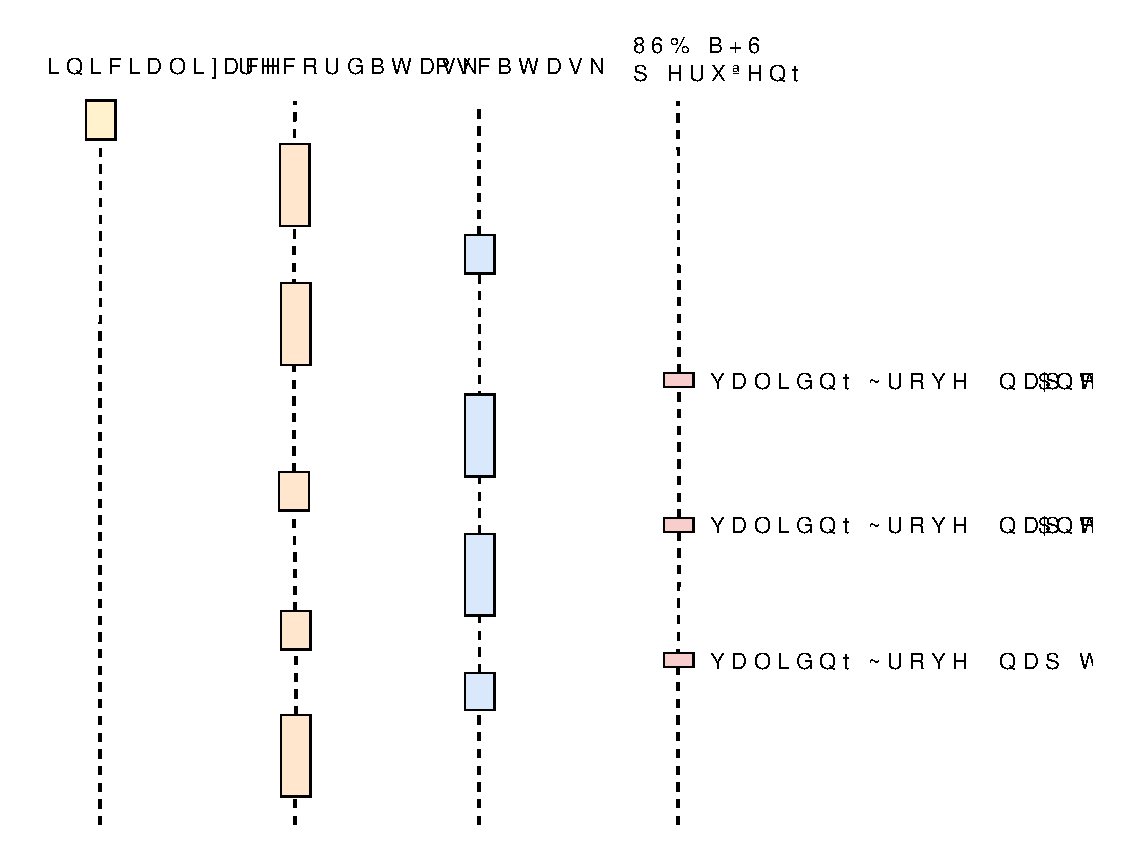
\includegraphics[width=1.00\textwidth]{obrazky-figures/run_wout_freertos.pdf}
    
    \caption{Zjednuduššený diagram běhu a přepínání úloh}
    \label{fig:run-wout-freertos}
\end{figure}

\newpage

\section{Záznamová úloha}
\label{zaznamove_vlakno}
% TODO: uvod + konfigurace zaznamu za behu DONE
% TODO: Napsat ze modul pro zaznam je ulozen v souboru record.c a record.h DONE
% TODO: upravit mluvi se dvakrat o UARTu! Asi CHILL
% uvest ze data jsou jednotlive znaky DONE
Samotná záznamová úloha je implementována v souboru \textit{app\_tasks.c}, přičemž využívá modul, poskytující funkce k záznamu dat, který je implementován v souborech \textit{record.c} a \textit{record.h}. 

% TODO: Inicializace WHERE? DONE
Inicializační fáze záznamové úlohy v prvním kroku zajišťuje inicializaci SD karty pomocí funkce \texttt{USB\_DeviceModeInit()}, která v případě potřeby zajistí i její naformátování. Následně funkce \texttt{CONSOLELOG\_Init()} provede připojení (Mount) SD karty, nastaví aktuální pracovní jednotku a ověří existenci souborového systému. Pokud není souborový systém nalezen, automaticky provede jeho vytvoření. Poté je vytvořen hlavní relační adresář (Session Directory) pomocí funkce \texttt{CONSOLELOG\_CreateDirectory()}, do kterého budou ukládány záznamy z dané relace, která trvá, až do vypnutí digitálního záznamníku.

% Chování záznamové úlohy je ovlivněno během inicializační fáze záznamové úlohy prostřednictvím konfiguračního souboru \textit{config.txt}, který je očekáván v kořenovém adresáři souborového systému přímo na SDHC kartě digitálního záznamníku.

% TODO: Default hodnoty zaznamu - baudrate a filesize zminit DONE
Během inicializační fáze záznamové úlohy jsou také nastaveny parametry záznamu prostřednictvím konfiguračního souboru \textit{config.txt}, který je očekáván v kořenovém adresáři souborového systému přímo na SDHC kartě digitálního záznamníku. Jak již bylo zmíněno, zařízení je určeno pro záznam sériových dat, respektive jedno-bajtových znaků přenášených prostřednictvím rozhraní UART, přičemž právě toto rozhraní je možné skrze konfiguraci upravit, primárně tedy rychlost přenosu neboli baudrate. Kromě toho je možné upravit maximální velikost záznamu (záznamového souboru), konkrétně u této velikosti se počítá s násobkem 512 bajtů, neboť data jsou ukládána po blocích (viz. kapitola \ref{davkove_zpracovani}), nicméně je možné zvolit i jinou hodnotu, přičemž firmware ji automaticky zaokrouhlí směrem nahoru na nejbližší přípustný násobek. V případě, že konfigurační soubor \textit{config.txt} není nalezen v kořenovém adresáři nebo se jeho obsah nepodaří záznamníku zpracovat, záznam zařízení proběhne dle předdefinovaných parametrů \texttt{DEFAULT\_BAUDRATE} a \texttt{DEFAULT\_MAX\_FILESIZE} uvedených v souboru \textit{defs.h}. Pro zpracování konfiguračního souboru slouží vlastní parser, který lze snadno rozšířit o podporu dalších parametrů.

% TODO: napsat jak vypada struktura logovani, vytvoreni slozky pro danou session, ....
%  v podobě mutexu, zatímco vnitřní smyčka vykonává vlastní záznamovou logiku...
Po přípravné fázi následuje samotná logika záznamu, ta je složena ze dvou smyček - vnější a vnitřní. Vnější smyčka reprezentuje řídicí smyčku úlohy, která čeká na aktivaci pomocí synchronizačního mechanismu, tedy binárního semaforu, zatímco vnitřní smyčka zprostředkovává záznam dat, ukládání dat do SDHC karty a případně signalizuje stav záznamu uživateli.

% V obsluze preruseni je take evidovan pocet tiku pri kterych byly data (bajt) zaznamenan
Samotný záznam dat je založen na konceptech představených v kapitole \ref{klicove_koncepty_digitalnich_zaznamniku}. V prvé řadě se jako vstupní periférie, sloužící k získání dat, využívá periférie LP\_FLEXCOMM (Low-Power Flexible Communications Interface) s přerušením. Zaznamenané jednotlivé znaky jsou v obslužné rutině přerušení vkládány do cirkulární vyrovnávací paměti, respektive softwarové FIFO fronty (viz. kapitola \ref{cirkularni_buffer}), se kterou je aktualizována hodnota zápisového ukazatele a také hodnota proměnné, která v sobě uchovává počet tiků, ve kterém data byla zaznamenána na základě systémového časového údaje vyjádřeného v tikách operačního systému.

Data jsou následně v běhu záznamové úlohy vkládána do jedné ze dvou vyrovnávacích pamětí, u kterých se využívá koncept vícenásobné vyrovnávací paměti (viz. kapitola \ref{vicenasobna_vyrovnavaci_pamet}), přičemž jedna paměť vždy slouží ke sběru a předzpracování přicházejících dat (tzv. aktivní buffer), zatímco druhá slouží k jejich ukládání na paměťovou kartu prostřednictvím řadiče SDHC. Role těchto dvou pamětí jsou mezi sebou cyklicky prohazovány na základě jednoduché výměny ukazatelů. Znaky jsou tedy vkládány do aktivního bufferu a při vkládání je každý nový znak porovnáván s předchozím tak, aby bylo možné detekovat přítomnost znakové dvojice \texttt{CR+LF} z prostředí operačního systému Windows CR+LF (Carriage Return Line Feed). Tento bílý znak je detekován z toho důvodu, že sledované zařízení používá znakové dvojice \texttt{CR+LF} pro ukončení řádku. Díky jeho rozpoznání je tak možné jednoznačně identifikovat začátek nového řádku. V případě, že je tato znaková sekvence zachycena, je z interního obvodu reálného času mikrokontroléru MCXN947 získán aktuální čas, který je následně vložen jako časová značka na začátek právě detekovaného řádku. Výsledný formát textu může vypadat následovně:

\begin{verbatim}
[12:34:56] Starting system diagnostics...
[12:34:57] Sensor reading: 23.5°C
[12:34:58] Data transmission OK
[12:34:59] System idle
\end{verbatim}

% U ADMA uvest ze to je neblokujici zpusob
% Uvest ze cela tato cast je implementovana funkci CONSOLELOG_Recording()
Aktivní buffer je tímto způsobem postupně plněn záznamovými daty a doplňován o časové značky s aktuálním časem. Jakmile dojde k jeho naplnění, jsou role obou vyrovnávacích pamětí vzájemně zaměněny prostou výměnou ukazatelů. Paměť, která dosud sloužila jako aktivní, je nyní určena k zápisu dat na SD kartu, a naopak – paměť předtím vyhrazená pro zápis se stává novým aktivním bufferem, připraveným přijímat další příchozí znaky. Samotný zápis dat do paměťového média je realizován neblokujícím způsobem prostřednictvím transportního algoritmu s přímým přístupem do paměti ADMA (Advanced Direct Memory Access). \cite{nxp_MCX_Nx4x_Reference_Manual}

Jakmile je záznamový soubor zaplněn na jeho maximální definovanou velikost, je soubor uzavřen, a následně je vytvořen nový pomocí funkce \texttt{CONSOLELOG\_CreateFile()}. Tato funkce na základě aktuálního data a času vygeneruje unikátní název souboru ve formátu \texttt{YYYYMMDD\_HHMMSS\_X.txt}, kde \texttt{X} je inkrementální čítač a následně tento soubor otevře pro zápis a nastaví jeho metadata (čas vytvoření) pomocí dat z interního RTC a záznam tak může pokračovat.

% je pojisteno ze kontrola CRLF probehne validne i v pripade ze je obsazeno ve dvou bufferech
Součástí návrhu je také ošetření okrajových stavů, které by mohly ohrozit konzistenci vkládání časových značek do záznamu. Typickým případem je rozdělení sekvence znaků, kdy první speciální znak \texttt{CR} se může dostat na konec vyrovnávací paměti plnící roli aktivního bufferu, následně dojde k prohození vyrovnávacích pamětí a druhý speciální znak \texttt{LF} se ocitne již na začátku nového aktivního bufferu. V takové situaci by se mohlo stát, že začátek řádku by nebyl detekován a časová značka by nebyla vložena. Aby bylo této chybě zabráněno, jsou uchovávány jakékoliv po sobě jdoucí znaky, a tedy k této situaci nedojde. Druhou situací je případ, kdy se sekvence \texttt{CR+LF} nachází na samotném konci aktivního bufferu a do dané paměti se již nevejde celá časová značka. Časová značka je v takovém případě rozdělena, část je uložena do konce původního bufferu a zbývající část je po výměně bufferů doplněna do nově aktivní paměti.

Další specifickou situací je potřeba korektního ukončení záznamu, tu lze například řešit pomocí tlačítka, nicméně rozhodl jsem se tuto situaci řešit obdobně jako situaci, kdy dojde ke ztrátě spojení s monitorovaným zařízením, která je z pohledu popisovaného algoritmu kritická. V takovém případě, totiž když není aktivní vyrovnávací paměť plně zaplněna, tak není uložena do permanentního uložiště, ale uvázne ve volatilní paměti digitálního záznamníku. Pro obě zmíněné situace je využívána funkce \texttt{CONSOLELOG\_Flush()},  která je periodicky volána a zajišťuje pravidelnou kontrolu, zda od posledního příjmu dat neuběhla doba specifikována makrem \texttt{FLUSH\_TIMEOUT\_TICKS} které je v základě nastaveno na dobu tří sekund. Po uplynutí této doby je automaticky obsah aktivního bufferu doplňen o bílé znaky v podobě mezery a obsah je uložen na SD kartu.

% TODO: napsat jak vypada struktura logovani, vytvoreni slozky pro danou session, ....
\begin{lstlisting}[language=C, caption={Pseudokód funkce \texttt{record\_task}}, label={lst:record_task}]
void record_task(void *handle)
{
    uint32_t baudrate = 0;
    uint32_t filesize = 0;

    USB_DeviceModeInit();

    CONSOLELOG_Init();

    if (CONSOLELOG_ReadConfig() != ERROR_NONE) {
        baudrate = DEFAULT_BAUDRATE;
        filesize = DEFAULT_MAX_FILESIZE;
    } else {s
        baudrate = CONSOLELOG_GetBaudrate();
        filesize = CONSOLELOG_GetFileSize();
    }

    while (1) {
        xSemaphoreTake(g_xSemRecord, portMAX_DELAY);

        UART_Init(baudrate);
        UART_Enable();

        while (1) {
            CONSOLELOG_Recording(filesize);
            
            LED_SignalRecording();

            CONSOLELOG_Flush()
        }
    }
}
\end{lstlisting}

\section{USB Mass Storage úloha}
Druhou úlohou je USB Mass Storage, která slouží ke zpřístupnění obsahu paměťové karty SDHC připojenému hostitelskému zařízení prostřednictvím rozhraní USB. Tato úloha je aktivována tehdy, když dojde k připojení záznamníku k hostitelskému zařízení USB1\_HS.

% zachovan pouze EHCI, z duvodu zjednodusseni projektu 
Funkcionalita USB Mass Storage je mnohdy poskytována samotnými výrobci mikrokontrolérů jako součást vývojových balíků s cílem usnadnit vývojářům vývoj aplikací. Společnost NXP Semiconductors nabízí v rámci svého MCUXpresso SDK (Software Development Kit) USB Mass Storage se zpřístupněním obsahu SD karty připojenému hostitelskému zařízení.

Bylo tedy třeba zaintegrovat USB Mass Storage do firmwaru digitálního záznamníku, ve kterém je veškerá paměť předalokována staticky. USB Mass Storage je v rámci projektu umístěn v adresáři \texttt{msc/}, dále je součástí v rámci složky \texttt{source/}, soubor \texttt{mass\_storage.c} obsahuje aplikaci USB Mass Storage, kterou je možné rozšířit. Z pohledu Mass Storage je také důležitá obslužná rutina přerušení \texttt{USB1\_Hs\_IRQHandler()}, která zprostředkovává komunikaci a přenos dat mezi hostitelským zařízením.

USB Mass Storage využívá obecný USB modul implementovaný se záměrem kompatibility s velkou řadou mikrokontrolérů. z tohoto důvodu jsem se rozhodl modul optimalizovat. Poskytnutý Mass Storage poskytuje vícero rozhraní hostitelských řadičů (Host Controller Interface - HCI) jakým je například KHCI, a speciální rozhraní pro rodinu LPC, které jsou nekompatibilní s mikrokontrolérem MCXN947, proto byla odstraněna, a v případě přechodu na jiné MCU lze rozhraní zaměnit. 

% Tato volba mi přijde jako vhodná, z tohoto důvodu, že není třeba periodicky kontrolovat napětí v systému (tzv. Polling), ale pouze pomocí přerušení, a lze tuto detekci upravovat pouze pomocí firmwaru.
% implementována v samostatném modulu \texttt{pwrloss_det.c}.
\section{Detekce ztráty napájejícího napětí}
Z důvodu prevence ztráty dat a minimalního rizika poškození souborového systému v důsledku náhlého výpadku napájení je v systému implementován mechanismus pro detekci poklesu napájecího napětí, který je realizován pomocí analogového komparátoru a pomocného časovače.  

Analogový komparátor je přítomen na MCU MCXN947 v podobě periferie \texttt{LPCMP} (Low-Power Comparator), který bude porovnávat napětí na \SI{5}{\volt} větvi, na které bude respektive hodnota napětí \SI{4.6}{\volt}, z důvodu úbytku napětí na Schottky diodě (viz. kapitola~\ref{zalohovane_napajeni_hw}).

Důležité je také zmínit, že v případě, kdy je zařízení napájeno, je napětí na sledované \SI{5}{\volt} napájecí větvi reálně nižší, a to přibližně \SI{4.6}{\volt} (viz. kapitola~\ref{zalohovane_napajeni_hw}) z důvodu úbytku napětí na Schottkyho diodě. Napětí z této větve je následně přivedeno na vstup analogového komparátoru prostřednictvím napěťového děliče. Komparátor musí reagovat co nejdříve, aby MCU dostalo co nejvíce času na uložení dat do SD karty, proto je jako hodnota napětí, při které bude komparátor reagovat, zvoleno napětí \SI{4.5}{\volt}, pokud je tato hodnota přepočítána na hodnotu napětí, které je za napěťovým děličem, vyjde hodnota \SI{2.91176}{\volt}, jelikož:

\begin{equation}
    V_{diff} = \SI{4.5}{\volt} * \frac{33}{18 + 33} = \SI{2.91176}{\volt} 
    \label{eq:trigger-cmp-val}
\end{equation}

Perifie \texttt{LPCMP} obsahuje interní DAC (Digital-Analog Converter), díky kterému je možné porovnávat vstupní analogový signál s 256 respektive 255 úrovněmi referenčního napětí, kterým je signál \texttt{VDD\_ANA} s napětím \SI{3.3}{\volt}. Z tohoto důvodu je hodnota v DAC, při které bude komparátor reagovat, nastavena na hexadecimální hodnotu 0xE1, jelikož:

\begin{equation}
    DAC_{level} = 255 * \frac{2.91176}{3.3} = 225.125 = 0xE1
    \label{eq:dac-value}
\end{equation}

% 5 tau = 16.5 sekundy
Reakce komparátoru je rovněž ovlivněna hysterézí nastavené na hodnotu \SI{20}{\milli\volt} aby byly omezeny falešné detekce. Krom samotného komparátoru je součástí detekce ztráty napájení ještě časovač, který za dobu $5\tau$ (čas, ve kterém bude kondenzátor pro zálohované napájení nabit na $99\%$) uvede komparátor do stavu, ve kterém je schopen detekovat korektně ztrátu napájení. Během testování se v ojedinělých případech objevily falešné detekce, pokud byl digitální záznamník napájen z měkkého zdroje a obvod pro zálohované napájení ještě nebyl dostatečně nabitý.\footnote{Stav, kdy je komparátor připraven k detekci, je signalizován pomocí LED (viz. kapitola \ref{signalizace_stavu_systemu}).}

Jakmile je záznamník připraven na bezpečné odpojení napájení, a k odpojení skutečně dojde, je pomocí komparátoru detekován pokles napětí pod stanovenou hranici a je vyvoláno přerušení od komparátoru s nejvyšší prioritou. Během obslužné rutiny přerušení jsou uložena všechna data, která jsou dočasně uložená ve volatilní paměti RAM, do souboru uloženém na SD kartě prostřednictvím funkce \texttt{CONSOLELOG\_Flush()}, která zajišťuje také korektní uzavření souboru. Následně se systém dostává do stavu, kdy je připraven na nedostatečné napětí, při kterém již není možný provoz záznamníku bez ohrožení integrity dat.

Na následujícím obrázku \ref{fig:pwrloss-detection-saleae} je možné vidět, jak komparátor reaguje v případě odpojení napájejícího napětí. Vrchní průběh grafu reprezentuje stav komparátoru, prostřední průběh zobrazuje napětí na vstupu komparátoru a poslední (spodní) reprezentuje stav napětí na sledované \SI{5}{\volt} napájecí větvi.

\begin{figure}[h]
    \centering
    \includegraphics[width=0.95\textwidth]{obrazky-figures/pwrloss-detection-saleae.png}`
    
    \caption{Zjednuduššený diagram běhu a přepínání úloh}
    \label{fig:pwrloss-detection-saleae}
\end{figure}

\section{Signalizace stavu systému}
\label{signalizace_stavu_systemu}
Digitální záznamník využívá sadu pěti LED diod, které slouží k signalizaci stavu digitálního záznamníku uživateli. Na následujícím obrázku~\ref{fig:signal-diodes} je znázorněno umístění jednotlivých LED diod na těle zařízení. Diody jsou číselně označeny 1 až 5, aby bylo možné v následujícím textu i tabulce~\ref{tab:signal_leds} jednoznačně popsat jejich význam a způsob indikace.

\begin{figure}[h]
    \centering
    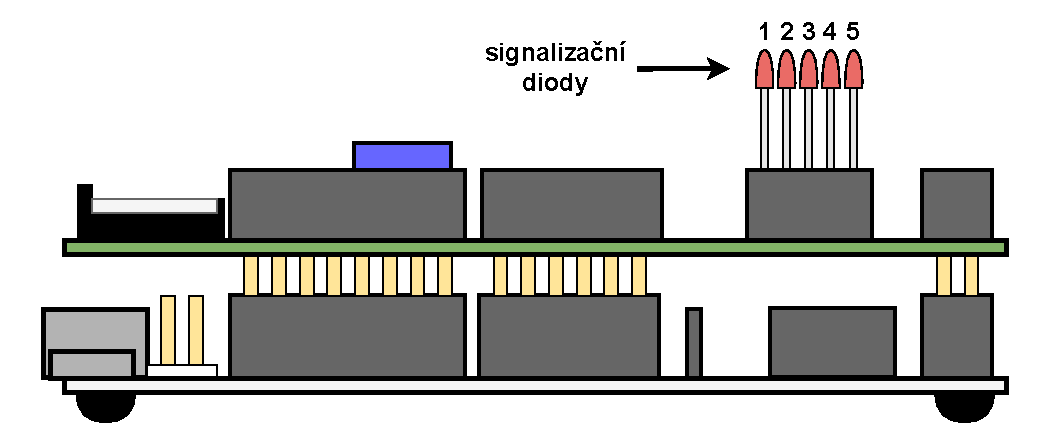
\includegraphics[width=1.00\textwidth]{obrazky-figures/signal_diodes.pdf}
    
    \caption{Zjednuduššený diagram běhu a přepínání úloh}
    \label{fig:signal-diodes}
\end{figure}

Dioda 1 signalizuje, zda je možné digitální záznamník bezpečně odpojit od napájejícího napětí a rozsvítí se tedy za dobu $5\tau$ (16.5 sekundy od připojení záznamníku k napájení), kdy je zajištěno dostatečné nabití kondenzátoru pro zálohované napájení. Dioda 4 signalizuje blikáním stav, kdy digitální záznamník zaznamenává a ukládá data. Pokud záznam skončí, tedy například monitorované zařízení přestane odesílat data, nebo je digitální záznamník odpojen od monitorovaného zařízení, rozsvítí se dioda 3. Může se stát, že na paměťové kartě nebude přítomen konfigurační soubor či bude ve špatném formátu, nebo může dojít k chybě během záznamu dat, v takovém případě je rozsvícená dioda 2.

Z pohledu uživatele je také důležité zjistit, zda digitální záznamník zaznamenává a ukládá data; k tomuto účelu slouží dioda 4, která v případě záznamu dat bliká. Pokud záznam skončí, tedy například monitorované zařízení přestane odesílat data, nebo je digitální záznamník odpojen od monitorovaného zařízení, rozsvítí se dioda 3. Může se stát, že na paměťové kartě nebude přítomen konfigurační soubor, či bude ve špatném formátu, nebo může dojít k chybě během záznamu dat; v takovém případě je rozsvícená dioda 2.
% 1 chybova dioda -> sviti pri chybe behem, ktereho neni mozne pokracovat v zaznamu dat
% 1 chybova dioda -> pokud napr chybi konfiguracni soubor, tedy je mozne napr. zaznamenavat data s zakladnim (default) nastavenim

\begin{table}[h]
    \centering
    \begin{tabular}{|c|c|c|}
        \hline
        \textbf{Dioda} & \textbf{Význam} & \textbf{Režim indikace} \\
        \hline
        D1 & Bezpečné odpojení & Svítí trvale  \\
        \hline
        D2 & Chybový stav během záznamu & Svítí trvale \\
        \hline
        D3 & Ukončení záznamu dat\footnote & Svítí trvale \\
        \hline
        D4 & Záznam aktivní & Bliká při záznamu dat \\
        \hline
        D5 & Ukončený záznam / bezpečné odpojení & Bliká po bezpečném uložení dat \\
        \hline
    \end{tabular}
    \caption{Přehled funkce jednotlivých signalizačních LED diod}
    \label{tab:signal_leds}
\end{table}

% ==================================================== 
\chapter{Testování systému}
\label{testovani_systemu}
% ----------------------------------------------------

\section{Funkcionální testování systému}
Funkcionalita digitálního záznamníku byla prověřena pomocí skriptu využívajícího objektově orientovaný přístup napsaném v jazyce Python. Tento skript simuluje monitorované zařízení tak, že načítá testovací textové soubory a jejich obsah postupně odesílá ve formě sériových dat přes COM port do digitálního záznamníku. Testovací skript se nachází v adresáři \texttt{tests/} pod názvem \texttt{serial\_test.py} a pro jejich korektní funkcionalitu je potřeba správně nastavit hodnoty definující, určující COM port, sadu testovacích souborů a přenosovou rychlost.

Testování s pomocí skriptu bylo prováděno s různými přenosovými rychlostmi, přičemž primárně bylo zaměřeno na přenosové rychlosti odpovídající skutečným scénářům nasazení. Během funkcionálního testování nebyla pozorována žádná ztráta dat.

Digitální záznamník byl rovněž testován spolu s reálným monitorovaným zařízením, 

\section{Kontrola bezpečnosti kódu}
Kromě funkcionálního testování byla provedena statická analýza zdrojového kódu pomocí pravidel specifikace MISRA C:2012. K tomuto účelu byla využita nástroj PC-lint Plus ve verzi 2.2 od společnosti Vector s 14denní licencí zdarma. Konfigurační soubory jsou společně s výstupy PC-lint Plus uloženy v adresáři \texttt{test/static-analysis/}. Pozornost byla věnována primárně pravidlům spadajícím do kategorie Required a Mandatory.\footnote{Pravidla ze skupiny Advisory nebyly brány v potaz, tyto chyby nijak nenarušují fukcionalitu firmwaru.} Většina porušení pravidel byla opravena a nebo obhájena pomocí komentáře, příčinu a důvod porušení pravidla (viz. ukázka~\ref{lst:misra}). Obhájená porušení se týkají zejména kvůli architektuře MCUXpresso SDK, FreeRTOSu či z důvodu, že PC-lint Plus nedokázal najít souvislosti mezi zdrojovými a hlavičkovými soubory.

\begin{lstlisting}[language=C, caption={Ukázka odůvodněného porušení pravidla MISRA}, label={lst:misra}]
/* MISRA Deviation Note:
 * Rule: MISRA 2012 Rule 10.3 [Required]
 * Justification: The enum value is part of the NXP SDK
 * and is intentionally used in this context as a bitmask flag for hardware 
 *  status registers.
 */
/*lint -e9034 MISRA Deviation: conversion from enum to unsigned32 */
CTIMER_ClearStatusFlags(CTIMER4, kCTIMER_Match0Flag);
/*lint +e9034 */
\end{lstlisting}

% ----------------------------------------------------

\section{Limitace systému}
\label{limitace}
    
% ----------------------------------------------------

\section{Možná rozšíření záznamníku}
\label{mozne_rozsireni}

\chapter{Závěr}
\label{zaver}


%===============================================================================

% Pro kompilaci po částech (viz projekt.tex) nutno odkomentovat
%\end{document}
